% Options for packages loaded elsewhere
\PassOptionsToPackage{unicode}{hyperref}
\PassOptionsToPackage{hyphens}{url}
%
\documentclass[
]{article}
\usepackage{amsmath,amssymb}
\usepackage{lmodern}
\usepackage{ifxetex,ifluatex}
\ifnum 0\ifxetex 1\fi\ifluatex 1\fi=0 % if pdftex
  \usepackage[T1]{fontenc}
  \usepackage[utf8]{inputenc}
  \usepackage{textcomp} % provide euro and other symbols
\else % if luatex or xetex
  \usepackage{unicode-math}
  \defaultfontfeatures{Scale=MatchLowercase}
  \defaultfontfeatures[\rmfamily]{Ligatures=TeX,Scale=1}
\fi
% Use upquote if available, for straight quotes in verbatim environments
\IfFileExists{upquote.sty}{\usepackage{upquote}}{}
\IfFileExists{microtype.sty}{% use microtype if available
  \usepackage[]{microtype}
  \UseMicrotypeSet[protrusion]{basicmath} % disable protrusion for tt fonts
}{}
\makeatletter
\@ifundefined{KOMAClassName}{% if non-KOMA class
  \IfFileExists{parskip.sty}{%
    \usepackage{parskip}
  }{% else
    \setlength{\parindent}{0pt}
    \setlength{\parskip}{6pt plus 2pt minus 1pt}}
}{% if KOMA class
  \KOMAoptions{parskip=half}}
\makeatother
\usepackage{xcolor}
\IfFileExists{xurl.sty}{\usepackage{xurl}}{} % add URL line breaks if available
\IfFileExists{bookmark.sty}{\usepackage{bookmark}}{\usepackage{hyperref}}
\hypersetup{
  pdftitle={TSST LMM},
  pdfauthor={AGC},
  hidelinks,
  pdfcreator={LaTeX via pandoc}}
\urlstyle{same} % disable monospaced font for URLs
\usepackage[margin=1in]{geometry}
\usepackage{color}
\usepackage{fancyvrb}
\newcommand{\VerbBar}{|}
\newcommand{\VERB}{\Verb[commandchars=\\\{\}]}
\DefineVerbatimEnvironment{Highlighting}{Verbatim}{commandchars=\\\{\}}
% Add ',fontsize=\small' for more characters per line
\usepackage{framed}
\definecolor{shadecolor}{RGB}{248,248,248}
\newenvironment{Shaded}{\begin{snugshade}}{\end{snugshade}}
\newcommand{\AlertTok}[1]{\textcolor[rgb]{0.94,0.16,0.16}{#1}}
\newcommand{\AnnotationTok}[1]{\textcolor[rgb]{0.56,0.35,0.01}{\textbf{\textit{#1}}}}
\newcommand{\AttributeTok}[1]{\textcolor[rgb]{0.77,0.63,0.00}{#1}}
\newcommand{\BaseNTok}[1]{\textcolor[rgb]{0.00,0.00,0.81}{#1}}
\newcommand{\BuiltInTok}[1]{#1}
\newcommand{\CharTok}[1]{\textcolor[rgb]{0.31,0.60,0.02}{#1}}
\newcommand{\CommentTok}[1]{\textcolor[rgb]{0.56,0.35,0.01}{\textit{#1}}}
\newcommand{\CommentVarTok}[1]{\textcolor[rgb]{0.56,0.35,0.01}{\textbf{\textit{#1}}}}
\newcommand{\ConstantTok}[1]{\textcolor[rgb]{0.00,0.00,0.00}{#1}}
\newcommand{\ControlFlowTok}[1]{\textcolor[rgb]{0.13,0.29,0.53}{\textbf{#1}}}
\newcommand{\DataTypeTok}[1]{\textcolor[rgb]{0.13,0.29,0.53}{#1}}
\newcommand{\DecValTok}[1]{\textcolor[rgb]{0.00,0.00,0.81}{#1}}
\newcommand{\DocumentationTok}[1]{\textcolor[rgb]{0.56,0.35,0.01}{\textbf{\textit{#1}}}}
\newcommand{\ErrorTok}[1]{\textcolor[rgb]{0.64,0.00,0.00}{\textbf{#1}}}
\newcommand{\ExtensionTok}[1]{#1}
\newcommand{\FloatTok}[1]{\textcolor[rgb]{0.00,0.00,0.81}{#1}}
\newcommand{\FunctionTok}[1]{\textcolor[rgb]{0.00,0.00,0.00}{#1}}
\newcommand{\ImportTok}[1]{#1}
\newcommand{\InformationTok}[1]{\textcolor[rgb]{0.56,0.35,0.01}{\textbf{\textit{#1}}}}
\newcommand{\KeywordTok}[1]{\textcolor[rgb]{0.13,0.29,0.53}{\textbf{#1}}}
\newcommand{\NormalTok}[1]{#1}
\newcommand{\OperatorTok}[1]{\textcolor[rgb]{0.81,0.36,0.00}{\textbf{#1}}}
\newcommand{\OtherTok}[1]{\textcolor[rgb]{0.56,0.35,0.01}{#1}}
\newcommand{\PreprocessorTok}[1]{\textcolor[rgb]{0.56,0.35,0.01}{\textit{#1}}}
\newcommand{\RegionMarkerTok}[1]{#1}
\newcommand{\SpecialCharTok}[1]{\textcolor[rgb]{0.00,0.00,0.00}{#1}}
\newcommand{\SpecialStringTok}[1]{\textcolor[rgb]{0.31,0.60,0.02}{#1}}
\newcommand{\StringTok}[1]{\textcolor[rgb]{0.31,0.60,0.02}{#1}}
\newcommand{\VariableTok}[1]{\textcolor[rgb]{0.00,0.00,0.00}{#1}}
\newcommand{\VerbatimStringTok}[1]{\textcolor[rgb]{0.31,0.60,0.02}{#1}}
\newcommand{\WarningTok}[1]{\textcolor[rgb]{0.56,0.35,0.01}{\textbf{\textit{#1}}}}
\usepackage{graphicx}
\makeatletter
\def\maxwidth{\ifdim\Gin@nat@width>\linewidth\linewidth\else\Gin@nat@width\fi}
\def\maxheight{\ifdim\Gin@nat@height>\textheight\textheight\else\Gin@nat@height\fi}
\makeatother
% Scale images if necessary, so that they will not overflow the page
% margins by default, and it is still possible to overwrite the defaults
% using explicit options in \includegraphics[width, height, ...]{}
\setkeys{Gin}{width=\maxwidth,height=\maxheight,keepaspectratio}
% Set default figure placement to htbp
\makeatletter
\def\fps@figure{htbp}
\makeatother
\setlength{\emergencystretch}{3em} % prevent overfull lines
\providecommand{\tightlist}{%
  \setlength{\itemsep}{0pt}\setlength{\parskip}{0pt}}
\setcounter{secnumdepth}{-\maxdimen} % remove section numbering
\ifluatex
  \usepackage{selnolig}  % disable illegal ligatures
\fi

\title{TSST LMM}
\author{AGC}
\date{15 4 2021}

\begin{document}
\maketitle

\hypertarget{prepare}{%
\section{Prepare}\label{prepare}}

\hypertarget{definitions}{%
\subsection{Definitions}\label{definitions}}

\textbf{IV of interest :}

\begin{itemize}
\tightlist
\item
  Gruppe (``group'')
\item
  sex (``gender'')
\item
  Zeitpunkt (``Time'') with 2xpolynomes
\item
  Gruppe x Zeitpunkt(each poly)
\item
  Gruppe x sex
\item
  Gruppe x sex x Time
\end{itemize}

\textbf{IV of no interest :}

\begin{itemize}
\tightlist
\item
  Age scaled (``age\_meancentered'')
\item
  ``explstart\_meancentered\_min''
\item
  ``BMI\_imp\_meancentered''
\item
  ``any\_med\_ccept''
\item
  ``smoking\_yes\_no''
\end{itemize}

\textbf{random effects} * Site (``centre'') * individual id

\textbf{DV:}

\begin{itemize}
\tightlist
\item
  psychologischer Stress („stressed")
\item
  Cortisol („CORT")
\item
  Testosteron („TEST")
\item
  Oxytocin (OXT")
\item
  log(TEST/CORT)
\end{itemize}

\textbf{sensitivity check}

\begin{itemize}
\tightlist
\item
  quantitative CD {[}instead of group{]}
\item
  gender
\item
  IQ
\item
  Parental education
\item
  pubertal status
\item
  ADHD lifetime diagnosis
\item
  Depression lifetime diagnosis
\item
  PTSD lifetime diagnosis
\item
  SUD lifetime diagnosis
\item
  Anxiety lifetime diagnosis
\end{itemize}

\hypertarget{read-and-check-data}{%
\subsection{read and check data}\label{read-and-check-data}}

\begin{Shaded}
\begin{Highlighting}[]
\CommentTok{\#df = as.data.frame(read\_sav(paste0(home,"/data/13.04.2021\_290\_170\_CORTAUCsplit.sav")))}

\NormalTok{df }\OtherTok{=} \FunctionTok{as.data.frame}\NormalTok{(}\FunctionTok{read\_sav}\NormalTok{(}\StringTok{"C:/Users/andreas\_chiocchetti/Documents/13.04.2021\_290\_170\_CORTAUCsplit.sav"}\NormalTok{))}

\NormalTok{df}\SpecialCharTok{$}\NormalTok{group }\OtherTok{=} \FunctionTok{drop}\NormalTok{(}\FunctionTok{factor}\NormalTok{(df}\SpecialCharTok{$}\NormalTok{group, }\AttributeTok{levels =} \FunctionTok{c}\NormalTok{(}\DecValTok{1}\NormalTok{,}\DecValTok{2}\NormalTok{), }\AttributeTok{labels=}\FunctionTok{c}\NormalTok{(}\StringTok{"CD"}\NormalTok{, }\StringTok{"HCs"}\NormalTok{))) }\SpecialCharTok{\%\textgreater{}\%} \FunctionTok{relevel}\NormalTok{(., }\AttributeTok{ref=}\StringTok{"HCs"}\NormalTok{)}
\NormalTok{df}\SpecialCharTok{$}\NormalTok{centre }\OtherTok{=} \FunctionTok{drop}\NormalTok{(}\FunctionTok{factor}\NormalTok{(df}\SpecialCharTok{$}\NormalTok{centre, }\AttributeTok{levels =} \FunctionTok{c}\NormalTok{(}\DecValTok{1}\NormalTok{,}\DecValTok{2}\NormalTok{,}\DecValTok{3}\NormalTok{,}\DecValTok{4}\NormalTok{,}\DecValTok{5}\NormalTok{), }\AttributeTok{labels=}\FunctionTok{c}\NormalTok{(}\StringTok{"Frankfurt"}\NormalTok{, }
                                                                   \StringTok{"Aachen"}\NormalTok{, }
                                                                   \StringTok{"Amsterdam"}\NormalTok{, }
                                                                   \StringTok{"SouthHampton"}\NormalTok{, }
                                                                   \StringTok{"Basel"}\NormalTok{)))}
\NormalTok{df}\SpecialCharTok{$}\NormalTok{twuid }\OtherTok{=} \FunctionTok{as.factor}\NormalTok{(df}\SpecialCharTok{$}\NormalTok{twuid)}



\NormalTok{df}\SpecialCharTok{$}\NormalTok{ADHD\_life }\OtherTok{=} \FunctionTok{drop}\NormalTok{(}\FunctionTok{factor}\NormalTok{(df}\SpecialCharTok{$}\NormalTok{ADHD\_life, }\AttributeTok{levels =} \FunctionTok{c}\NormalTok{(}\DecValTok{0}\NormalTok{,}\DecValTok{1}\NormalTok{), }
                               \AttributeTok{labels=}\FunctionTok{c}\NormalTok{(}\StringTok{"no\_ADHD"}\NormalTok{, }\StringTok{"ADHD"}\NormalTok{)))}\SpecialCharTok{\%\textgreater{}\%} \FunctionTok{relevel}\NormalTok{(., }\AttributeTok{ref=}\StringTok{"no\_ADHD"}\NormalTok{)}
\NormalTok{df}\SpecialCharTok{$}\NormalTok{Depression\_lifetime }\OtherTok{=} \FunctionTok{drop}\NormalTok{(}\FunctionTok{factor}\NormalTok{(df}\SpecialCharTok{$}\NormalTok{Depression\_lifetime, }\AttributeTok{levels =} \FunctionTok{c}\NormalTok{(}\DecValTok{0}\NormalTok{,}\DecValTok{1}\NormalTok{), }
                               \AttributeTok{labels=}\FunctionTok{c}\NormalTok{(}\StringTok{"no\_Depression"}\NormalTok{, }\StringTok{"Depression"}\NormalTok{)))}\SpecialCharTok{\%\textgreater{}\%} \FunctionTok{relevel}\NormalTok{(., }\AttributeTok{ref=}\StringTok{"no\_Depression"}\NormalTok{)}

\NormalTok{df}\SpecialCharTok{$}\NormalTok{PTSD\_lifetime }\OtherTok{=} \FunctionTok{drop}\NormalTok{(}\FunctionTok{factor}\NormalTok{(df}\SpecialCharTok{$}\NormalTok{PTSD\_lifetime, }\AttributeTok{levels =} \FunctionTok{c}\NormalTok{(}\DecValTok{0}\NormalTok{,}\DecValTok{1}\NormalTok{), }
                               \AttributeTok{labels=}\FunctionTok{c}\NormalTok{(}\StringTok{"no\_PTSD"}\NormalTok{, }\StringTok{"PTSD"}\NormalTok{)))}\SpecialCharTok{\%\textgreater{}\%} \FunctionTok{relevel}\NormalTok{(., }\AttributeTok{ref=}\StringTok{"no\_PTSD"}\NormalTok{)}
\NormalTok{df}\SpecialCharTok{$}\NormalTok{SUD\_life }\OtherTok{=} \FunctionTok{drop}\NormalTok{(}\FunctionTok{factor}\NormalTok{(df}\SpecialCharTok{$}\NormalTok{SUD\_life, }\AttributeTok{levels =} \FunctionTok{c}\NormalTok{(}\DecValTok{0}\NormalTok{,}\DecValTok{1}\NormalTok{), }
                               \AttributeTok{labels=}\FunctionTok{c}\NormalTok{(}\StringTok{"no\_SUD"}\NormalTok{, }\StringTok{"SUD"}\NormalTok{)))}\SpecialCharTok{\%\textgreater{}\%} \FunctionTok{relevel}\NormalTok{(., }\AttributeTok{ref=}\StringTok{"no\_SUD"}\NormalTok{)}

\NormalTok{df}\SpecialCharTok{$}\NormalTok{Anxiety\_lifetime }\OtherTok{=} \FunctionTok{drop}\NormalTok{(}\FunctionTok{factor}\NormalTok{(df}\SpecialCharTok{$}\NormalTok{Anxiety\_lifetime, }\AttributeTok{levels =} \FunctionTok{c}\NormalTok{(}\DecValTok{0}\NormalTok{,}\DecValTok{1}\NormalTok{), }
                               \AttributeTok{labels=}\FunctionTok{c}\NormalTok{(}\StringTok{"no\_Anxiety"}\NormalTok{, }\StringTok{"Anxiety"}\NormalTok{)))}\SpecialCharTok{\%\textgreater{}\%} \FunctionTok{relevel}\NormalTok{(., }\AttributeTok{ref=}\StringTok{"no\_Anxiety"}\NormalTok{)}

\NormalTok{df}\SpecialCharTok{$}\NormalTok{any\_med\_ccept }\OtherTok{=} \FunctionTok{drop}\NormalTok{(}\FunctionTok{factor}\NormalTok{(df}\SpecialCharTok{$}\NormalTok{any\_med\_ccept, }\AttributeTok{levels =} \FunctionTok{c}\NormalTok{(}\DecValTok{0}\NormalTok{,}\DecValTok{1}\NormalTok{), }
                               \AttributeTok{labels=}\FunctionTok{c}\NormalTok{(}\StringTok{"no\_med"}\NormalTok{, }\StringTok{"med"}\NormalTok{)))}\SpecialCharTok{\%\textgreater{}\%} \FunctionTok{relevel}\NormalTok{(., }\AttributeTok{ref=}\StringTok{"no\_med"}\NormalTok{)}
\NormalTok{df}\SpecialCharTok{$}\NormalTok{smoking\_yes\_no }\OtherTok{=} \FunctionTok{drop}\NormalTok{(}\FunctionTok{factor}\NormalTok{(df}\SpecialCharTok{$}\NormalTok{smoking\_yes\_no, }\AttributeTok{levels =} \FunctionTok{c}\NormalTok{(}\DecValTok{0}\NormalTok{,}\DecValTok{1}\NormalTok{), }
                                \AttributeTok{labels=}\FunctionTok{c}\NormalTok{(}\StringTok{"no\_smk"}\NormalTok{, }\StringTok{"smk"}\NormalTok{)))}\SpecialCharTok{\%\textgreater{}\%} \FunctionTok{relevel}\NormalTok{(., }\AttributeTok{ref=}\StringTok{"no\_smk"}\NormalTok{)}
\NormalTok{df}\SpecialCharTok{$}\NormalTok{gender }\OtherTok{=} \FunctionTok{drop}\NormalTok{(}\FunctionTok{factor}\NormalTok{(df}\SpecialCharTok{$}\NormalTok{gender, }\AttributeTok{levels =} \FunctionTok{c}\NormalTok{(}\DecValTok{1}\NormalTok{,}\DecValTok{2}\NormalTok{), }
                        \AttributeTok{labels=}\FunctionTok{c}\NormalTok{(}\StringTok{"female"}\NormalTok{, }\StringTok{"male"}\NormalTok{)))}\SpecialCharTok{\%\textgreater{}\%} \FunctionTok{relevel}\NormalTok{(., }\AttributeTok{ref=}\StringTok{"male"}\NormalTok{)}

\CommentTok{\# table(df$group, useNA = "always")}
\CommentTok{\# table(df$centre, useNA = "always")}
\CommentTok{\# table(df$any\_med\_ccept, useNA = "always")}
\CommentTok{\# table(df$smoking\_yes\_no, useNA = "always")}
\CommentTok{\# table(df$gender, useNA = "always")}

\NormalTok{df}\SpecialCharTok{$}\NormalTok{TESTCORTlogBL }\OtherTok{=} \FunctionTok{log}\NormalTok{(df}\SpecialCharTok{$}\NormalTok{TEST\_BL\_log}\SpecialCharTok{/}\NormalTok{df}\SpecialCharTok{$}\NormalTok{CORT\_BL\_log)}
\NormalTok{df}\SpecialCharTok{$}\NormalTok{TESTCORTlogBL[}\FunctionTok{is.infinite}\NormalTok{(df}\SpecialCharTok{$}\NormalTok{TESTCORTlogBL)] }\OtherTok{=} \ConstantTok{NA}

\NormalTok{df}\SpecialCharTok{$}\NormalTok{TESTCORTlog10 }\OtherTok{=} \FunctionTok{log}\NormalTok{(df}\SpecialCharTok{$}\NormalTok{TEST\_10\_log}\SpecialCharTok{/}\NormalTok{df}\SpecialCharTok{$}\NormalTok{CORT\_10\_log)}
\NormalTok{df}\SpecialCharTok{$}\NormalTok{TESTCORTlog10[}\FunctionTok{is.infinite}\NormalTok{(df}\SpecialCharTok{$}\NormalTok{TESTCORTlog10)] }\OtherTok{=} \ConstantTok{NA}

\NormalTok{df}\SpecialCharTok{$}\NormalTok{TESTCORTlog55 }\OtherTok{=} \FunctionTok{log}\NormalTok{(df}\SpecialCharTok{$}\NormalTok{TEST\_55\_log}\SpecialCharTok{/}\NormalTok{df}\SpecialCharTok{$}\NormalTok{CORT\_55\_log)}
\NormalTok{df}\SpecialCharTok{$}\NormalTok{TESTCORTlog55[}\FunctionTok{is.infinite}\NormalTok{(df}\SpecialCharTok{$}\NormalTok{TESTCORTlog55)] }\OtherTok{=} \ConstantTok{NA}

\CommentTok{\# added mean centered}
\NormalTok{df}\SpecialCharTok{$}\NormalTok{dayslastmens\_meancentered }\OtherTok{=}\NormalTok{ df}\SpecialCharTok{$}\NormalTok{days\_since\_last\_mens}\SpecialCharTok{{-}}\FunctionTok{mean}\NormalTok{(df}\SpecialCharTok{$}\NormalTok{days\_since\_last\_mens, }\AttributeTok{na.rm=}\NormalTok{T)}

\NormalTok{UV }\OtherTok{=} \FunctionTok{c}\NormalTok{(}\StringTok{"centre"}\NormalTok{,}\StringTok{"age\_meancentered"}\NormalTok{, }\StringTok{"explstart\_meancentered\_min"}\NormalTok{, }
  \StringTok{"BMI\_imp\_meancentered"}\NormalTok{, }\StringTok{"any\_med\_ccept"}\NormalTok{, }\StringTok{"smoking\_yes\_no"}\NormalTok{, }\StringTok{"gender"}\NormalTok{, }\StringTok{"group"}\NormalTok{,}
  \StringTok{"CDsymptomscurrent"}\NormalTok{)}


\NormalTok{Sensvar }\OtherTok{=} \FunctionTok{c}\NormalTok{(}\StringTok{"iq\_e\_total\_imp\_meancentered"}\NormalTok{, }
           \StringTok{"EduParentsISCEDMean\_meancentered"}\NormalTok{,}
           \StringTok{"pubcatimp\_meancentered"}\NormalTok{,}
           \StringTok{"dayslastmens\_meancentered"}\NormalTok{,}
           \StringTok{"ADHD\_life"}\NormalTok{,}
           \StringTok{"Depression\_lifetime"}\NormalTok{,}
           \StringTok{"PTSD\_lifetime"}\NormalTok{,}
           \StringTok{"SUD\_life"}\NormalTok{,}
           \StringTok{"Anxiety\_lifetime"}\NormalTok{)}

\NormalTok{AV }\OtherTok{=} \FunctionTok{list}\NormalTok{(}
\AttributeTok{AV\_stressed =} \FunctionTok{c}\NormalTok{(}\AttributeTok{stressed\_1=}\DecValTok{0}\NormalTok{, }\AttributeTok{stressed\_2=}\DecValTok{2}\NormalTok{,}
                \AttributeTok{stressed\_3=}\DecValTok{10}\NormalTok{, }\AttributeTok{stressed\_4=}\DecValTok{16}\NormalTok{,}
                \AttributeTok{stressed\_5=}\DecValTok{25}\NormalTok{, }\AttributeTok{stressed\_6=}\DecValTok{40}\NormalTok{, }
                \AttributeTok{stressed\_7=}\DecValTok{55}\NormalTok{, }\AttributeTok{stressed\_8=}\DecValTok{70}\NormalTok{), }
\AttributeTok{AV\_CORT =} \FunctionTok{c}\NormalTok{(}\AttributeTok{CORT\_BL\_log=}\DecValTok{0}\NormalTok{, }\AttributeTok{CORT\_10\_log=}\DecValTok{25}\NormalTok{, }\AttributeTok{CORT\_25\_log=}\DecValTok{40}\NormalTok{, }\AttributeTok{CORT\_40\_log=}\DecValTok{55}\NormalTok{, }\AttributeTok{CORT\_55\_log=}\DecValTok{70}\NormalTok{) ,}
\AttributeTok{AV\_TEST =} \FunctionTok{c}\NormalTok{(}\AttributeTok{TEST\_BL\_log=}\DecValTok{0}\NormalTok{, }\AttributeTok{TEST\_10\_log=}\DecValTok{25}\NormalTok{, }\AttributeTok{TEST\_55\_log=}\DecValTok{70}\NormalTok{),}
\AttributeTok{AV\_TESTCORT =} \FunctionTok{c}\NormalTok{(}\AttributeTok{TESTCORTlogBL =} \DecValTok{0}\NormalTok{, }\AttributeTok{TESTCORTlog10=}\DecValTok{25}\NormalTok{, }\AttributeTok{TESTCORTlog55 =} \DecValTok{70}\NormalTok{),}
\AttributeTok{AV\_OXT =}  \FunctionTok{c}\NormalTok{(}\AttributeTok{OXT\_BL\_log=}\DecValTok{0}\NormalTok{, }\AttributeTok{OXT\_1\_log=}\DecValTok{16}\NormalTok{, }\AttributeTok{OXT\_10\_log=}\DecValTok{25}\NormalTok{))}

\NormalTok{vartoplot }\OtherTok{=} \FunctionTok{c}\NormalTok{(UV, Sensvar)}
\NormalTok{tmpframe }\OtherTok{=}\NormalTok{ df[,vartoplot[}\SpecialCharTok{!}\NormalTok{vartoplot}\SpecialCharTok{\%in\%} \FunctionTok{c}\NormalTok{(}\StringTok{"centre"}\NormalTok{)]] }\SpecialCharTok{\%\textgreater{}\%} \FunctionTok{mutate\_if}\NormalTok{(is.factor, }\ControlFlowTok{function}\NormalTok{(x) }\FunctionTok{as.numeric}\NormalTok{(x)}\SpecialCharTok{{-}}\DecValTok{1}\NormalTok{)}

\NormalTok{corrplot}\SpecialCharTok{::}\FunctionTok{corrplot}\NormalTok{(}\FunctionTok{cor}\NormalTok{(tmpframe, }\AttributeTok{use =} \StringTok{"pairwise"}\NormalTok{))}
\end{Highlighting}
\end{Shaded}

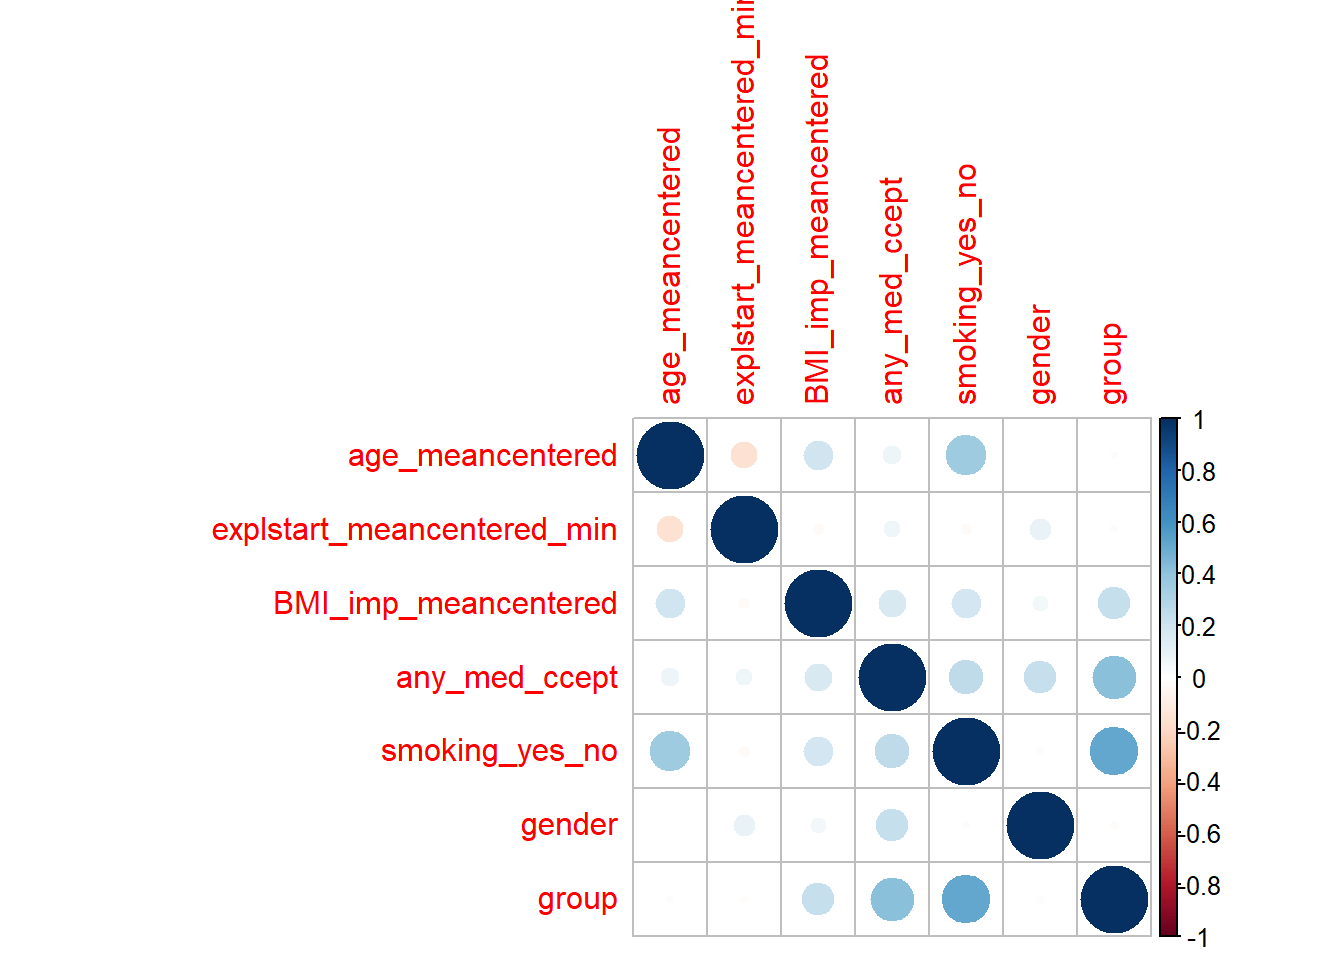
\includegraphics{01_Preprocessing_Modelling_files/figure-latex/preprocess-1.pdf}

\hypertarget{complete-cohort-descriptives}{%
\subsection{complete cohort
descriptives}\label{complete-cohort-descriptives}}

\begin{Shaded}
\begin{Highlighting}[]
\NormalTok{res }\OtherTok{=} \FunctionTok{compareGroups}\NormalTok{(group}\SpecialCharTok{\textasciitilde{}}\NormalTok{., }\AttributeTok{data =}\NormalTok{ df[,}\FunctionTok{c}\NormalTok{(UV, }\FunctionTok{unlist}\NormalTok{(}\FunctionTok{lapply}\NormalTok{(AV, names)), Sensvar)])}
\CommentTok{\#summary(res)}
\NormalTok{export\_table }\OtherTok{\textless{}{-}} \FunctionTok{createTable}\NormalTok{(res)}
\NormalTok{export\_table}
\end{Highlighting}
\end{Shaded}

\begin{verbatim}
## 
## --------Summary descriptives table by 'group'---------
## 
## ____________________________________________________________________ 
##                                      HCs           CD      p.overall 
##                                     N=160        N=130               
## ¯¯¯¯¯¯¯¯¯¯¯¯¯¯¯¯¯¯¯¯¯¯¯¯¯¯¯¯¯¯¯¯¯¯¯¯¯¯¯¯¯¯¯¯¯¯¯¯¯¯¯¯¯¯¯¯¯¯¯¯¯¯¯¯¯¯¯¯ 
## centre:                                                      0.013   
##     Frankfurt                     81 (50.6%)   63 (48.5%)            
##     Aachen                        5 (3.12%)    16 (12.3%)            
##     Amsterdam                     14 (8.75%)   15 (11.5%)            
##     SouthHampton                  32 (20.0%)   24 (18.5%)            
##     Basel                         28 (17.5%)   12 (9.23%)            
## age_meancentered                 -0.03 (2.07) 0.01 (1.78)    0.853   
## explstart_meancentered_min       1.66 (53.5)  -0.05 (55.5)   0.791   
## BMI_imp_meancentered             -0.98 (3.79) 1.31 (5.77)   <0.001   
## any_med_ccept:                                              <0.001   
##     no_med                       146 (91.2%)   72 (55.4%)            
##     med                           14 (8.75%)   58 (44.6%)            
## smoking_yes_no:                                             <0.001   
##     no_smk                       144 (90.0%)   54 (41.5%)            
##     smk                           16 (10.0%)   76 (58.5%)            
## gender:                                                      0.829   
##     male                          56 (35.0%)   48 (36.9%)            
##     female                       104 (65.0%)   82 (63.1%)            
## CDsymptomscurrent                0.07 (0.26)  5.25 (2.18)   <0.001   
## stressed_1                       1.12 (1.89)  1.48 (2.19)    0.135   
## stressed_2                       2.94 (2.86)  3.53 (3.26)    0.108   
## stressed_3                       3.24 (2.96)  3.74 (3.41)    0.188   
## stressed_4                       1.58 (2.31)  2.01 (2.58)    0.139   
## stressed_5                       0.57 (1.12)  1.09 (1.80)    0.004   
## stressed_6                       0.46 (1.03)  1.25 (2.15)   <0.001   
## stressed_7                       0.37 (0.85)  0.99 (1.98)    0.001   
## stressed_8                       0.35 (0.88)  0.95 (2.00)    0.002   
## CORT_BL_log                      0.87 (0.63)  0.97 (0.53)    0.121   
## CORT_10_log                      1.54 (0.77)  0.97 (0.61)   <0.001   
## CORT_25_log                      1.33 (0.74)  0.91 (0.57)   <0.001   
## CORT_40_log                      1.14 (0.67)  0.86 (0.54)   <0.001   
## CORT_55_log                      1.01 (0.65)  0.80 (0.55)    0.004   
## TEST_BL_log                      3.60 (0.57)  3.71 (0.56)    0.088   
## TEST_10_log                      3.79 (0.56)  3.74 (0.60)    0.479   
## TEST_55_log                      3.67 (0.59)  3.72 (0.63)    0.533   
## TESTCORTlogBL                    1.52 (0.71)  1.43 (0.74)    0.288   
## TESTCORTlog10                    1.02 (0.57)  1.42 (0.56)   <0.001   
## TESTCORTlog55                    1.40 (0.67)  1.57 (0.58)    0.026   
## OXT_BL_log                       0.18 (0.48)  0.15 (0.36)    0.639   
## OXT_1_log                        0.33 (0.53)  0.20 (0.36)    0.052   
## OXT_10_log                       0.26 (0.50)  0.28 (0.37)    0.810   
## iq_e_total_imp_meancentered      2.72 (12.0)  -3.35 (12.8)  <0.001   
## EduParentsISCEDMean_meancentered 0.29 (1.01)  -0.39 (0.88)  <0.001   
## pubcatimp_meancentered           -0.02 (0.86) 0.03 (0.79)    0.579   
## dayslastmens_meancentered        -0.49 (14.1) 0.58 (18.2)    0.719   
## ADHD_life:                                                  <0.001   
##     no_ADHD                       160 (100%)   71 (54.6%)            
##     ADHD                          0 (0.00%)    59 (45.4%)            
## Depression_lifetime:                                        <0.001   
##     no_Depression                156 (97.5%)   86 (66.2%)            
##     Depression                    4 (2.50%)    44 (33.8%)            
## PTSD_lifetime:                                              <0.001   
##     no_PTSD                      158 (98.8%)  114 (87.7%)            
##     PTSD                          2 (1.25%)    16 (12.3%)            
## SUD_life:                                                   <0.001   
##     no_SUD                       159 (99.4%)   98 (75.4%)            
##     SUD                           1 (0.62%)    32 (24.6%)            
## Anxiety_lifetime:                                           <0.001   
##     no_Anxiety                   156 (97.5%)   95 (73.1%)            
##     Anxiety                       4 (2.50%)    35 (26.9%)            
## ¯¯¯¯¯¯¯¯¯¯¯¯¯¯¯¯¯¯¯¯¯¯¯¯¯¯¯¯¯¯¯¯¯¯¯¯¯¯¯¯¯¯¯¯¯¯¯¯¯¯¯¯¯¯¯¯¯¯¯¯¯¯¯¯¯¯¯¯
\end{verbatim}

\hypertarget{male-only-cohort-descriptives}{%
\subsection{male only cohort
descriptives}\label{male-only-cohort-descriptives}}

\begin{Shaded}
\begin{Highlighting}[]
\NormalTok{res }\OtherTok{=} \FunctionTok{compareGroups}\NormalTok{(group}\SpecialCharTok{\textasciitilde{}}\NormalTok{., }\AttributeTok{data =}\NormalTok{ df[,}\FunctionTok{c}\NormalTok{(UV, }\FunctionTok{unlist}\NormalTok{(}\FunctionTok{lapply}\NormalTok{(AV, names)), Sensvar)], }
                    \AttributeTok{subset =}\NormalTok{ gender}\SpecialCharTok{==}\StringTok{"male"}\NormalTok{)}
\NormalTok{export\_table }\OtherTok{\textless{}{-}} \FunctionTok{createTable}\NormalTok{(res)}
\NormalTok{export\_table}
\end{Highlighting}
\end{Shaded}

\begin{verbatim}
## 
## --------Summary descriptives table by 'group'---------
## 
## _____________________________________________________________________ 
##                                       HCs           CD      p.overall 
##                                      N=56          N=48               
## ¯¯¯¯¯¯¯¯¯¯¯¯¯¯¯¯¯¯¯¯¯¯¯¯¯¯¯¯¯¯¯¯¯¯¯¯¯¯¯¯¯¯¯¯¯¯¯¯¯¯¯¯¯¯¯¯¯¯¯¯¯¯¯¯¯¯¯¯¯ 
## centre:                                                       0.452   
##     Frankfurt                     32 (57.1%)    34 (70.8%)            
##     Aachen                         3 (5.36%)    3 (6.25%)             
##     SouthHampton                  16 (28.6%)    8 (16.7%)             
##     Basel                          5 (8.93%)    3 (6.25%)             
## age_meancentered                  0.16 (2.06)  -0.17 (2.13)   0.422   
## explstart_meancentered_min       -10.88 (51.4) -0.88 (51.6)   0.326   
## BMI_imp_meancentered             -0.82 (3.55)  0.33 (4.03)    0.128   
## any_med_ccept:                                                0.015   
##     no_med                        54 (96.4%)    38 (79.2%)            
##     med                            2 (3.57%)    10 (20.8%)            
## smoking_yes_no:                                              <0.001   
##     no_smk                        47 (83.9%)    23 (47.9%)            
##     smk                            9 (16.1%)    25 (52.1%)            
## gender: male                       56 (100%)    48 (100%)       .     
## CDsymptomscurrent                 0.11 (0.31)  5.27 (2.36)   <0.001   
## stressed_1                        0.94 (1.69)  1.43 (1.65)    0.132   
## stressed_2                        2.34 (2.44)  2.86 (2.81)    0.321   
## stressed_3                        3.22 (2.84)  3.10 (3.10)    0.834   
## stressed_4                        1.24 (1.73)  1.82 (2.29)    0.151   
## stressed_5                        0.54 (1.10)  0.92 (1.33)    0.112   
## stressed_6                        0.37 (0.89)  1.14 (1.88)    0.011   
## stressed_7                        0.30 (0.67)  0.99 (1.72)    0.011   
## stressed_8                        0.26 (0.65)  0.94 (1.90)    0.022   
## CORT_BL_log                       1.05 (0.59)  1.01 (0.57)    0.750   
## CORT_10_log                       1.54 (0.82)  0.99 (0.56)   <0.001   
## CORT_25_log                       1.35 (0.80)  0.88 (0.57)    0.001   
## CORT_40_log                       1.17 (0.73)  0.86 (0.59)    0.020   
## CORT_55_log                       1.16 (0.68)  0.80 (0.61)    0.005   
## TEST_BL_log                       3.90 (0.60)  3.94 (0.63)    0.754   
## TEST_10_log                       4.02 (0.64)  3.99 (0.65)    0.807   
## TEST_55_log                       4.02 (0.64)  3.95 (0.80)    0.602   
## TESTCORTlogBL                     1.38 (0.59)  1.47 (0.59)    0.490   
## TESTCORTlog10                     1.10 (0.56)  1.52 (0.61)   <0.001   
## TESTCORTlog55                     1.36 (0.56)  1.63 (0.57)    0.019   
## OXT_BL_log                        0.11 (0.52)  0.02 (0.30)    0.368   
## OXT_1_log                         0.29 (0.52)  0.10 (0.32)    0.052   
## OXT_10_log                        0.19 (0.52)  0.18 (0.36)    0.904   
## iq_e_total_imp_meancentered       3.65 (11.7)  -0.89 (12.6)   0.061   
## EduParentsISCEDMean_meancentered  0.15 (0.92)  -0.20 (0.72)   0.042   
## pubcatimp_meancentered           -0.50 (0.88)  -0.47 (0.86)   0.848   
## dayslastmens_meancentered              .            .           .     
## ADHD_life:                                                   <0.001   
##     no_ADHD                        56 (100%)    20 (41.7%)            
##     ADHD                           0 (0.00%)    28 (58.3%)            
## Depression_lifetime:                                          0.001   
##     no_Depression                  56 (100%)    39 (81.2%)            
##     Depression                     0 (0.00%)    9 (18.8%)             
## PTSD_lifetime:                                                0.093   
##     no_PTSD                       55 (98.2%)    43 (89.6%)            
##     PTSD                           1 (1.79%)    5 (10.4%)             
## SUD_life:                                                    <0.001   
##     no_SUD                        55 (98.2%)    34 (70.8%)            
##     SUD                            1 (1.79%)    14 (29.2%)            
## Anxiety_lifetime:                                            <0.001   
##     no_Anxiety                    54 (96.4%)    31 (64.6%)            
##     Anxiety                        2 (3.57%)    17 (35.4%)            
## ¯¯¯¯¯¯¯¯¯¯¯¯¯¯¯¯¯¯¯¯¯¯¯¯¯¯¯¯¯¯¯¯¯¯¯¯¯¯¯¯¯¯¯¯¯¯¯¯¯¯¯¯¯¯¯¯¯¯¯¯¯¯¯¯¯¯¯¯¯
\end{verbatim}

\hypertarget{female-only-cohort-descriptives}{%
\subsection{female only cohort
descriptives}\label{female-only-cohort-descriptives}}

\begin{Shaded}
\begin{Highlighting}[]
\NormalTok{res }\OtherTok{=} \FunctionTok{compareGroups}\NormalTok{(group}\SpecialCharTok{\textasciitilde{}}\NormalTok{., }
                    \AttributeTok{data =}\NormalTok{ df[,}\FunctionTok{c}\NormalTok{(UV, }\FunctionTok{unlist}\NormalTok{(}\FunctionTok{lapply}\NormalTok{(AV, names)), Sensvar)], }
                    \AttributeTok{subset =}\NormalTok{ gender}\SpecialCharTok{==}\StringTok{"female"}\NormalTok{)}
\NormalTok{export\_table }\OtherTok{\textless{}{-}} \FunctionTok{createTable}\NormalTok{(res)}
\NormalTok{export\_table}
\end{Highlighting}
\end{Shaded}

\begin{verbatim}
## 
## --------Summary descriptives table by 'group'---------
## 
## ____________________________________________________________________ 
##                                      HCs           CD      p.overall 
##                                     N=104         N=82               
## ¯¯¯¯¯¯¯¯¯¯¯¯¯¯¯¯¯¯¯¯¯¯¯¯¯¯¯¯¯¯¯¯¯¯¯¯¯¯¯¯¯¯¯¯¯¯¯¯¯¯¯¯¯¯¯¯¯¯¯¯¯¯¯¯¯¯¯¯ 
## centre:                                                      0.002   
##     Frankfurt                     49 (47.1%)   29 (35.4%)            
##     Aachen                        2 (1.92%)    13 (15.9%)            
##     Amsterdam                     14 (13.5%)   15 (18.3%)            
##     SouthHampton                  16 (15.4%)   16 (19.5%)            
##     Basel                         23 (22.1%)   9 (11.0%)             
## age_meancentered                 -0.13 (2.07) 0.12 (1.54)    0.342   
## explstart_meancentered_min       8.40 (53.6)  0.43 (58.0)    0.337   
## BMI_imp_meancentered             -1.07 (3.92) 1.89 (6.54)   <0.001   
## any_med_ccept:                                              <0.001   
##     no_med                        92 (88.5%)   34 (41.5%)            
##     med                           12 (11.5%)   48 (58.5%)            
## smoking_yes_no:                                             <0.001   
##     no_smk                        97 (93.3%)   31 (37.8%)            
##     smk                           7 (6.73%)    51 (62.2%)            
## gender: female                    104 (100%)   82 (100%)       .     
## CDsymptomscurrent                0.06 (0.23)  5.23 (2.08)   <0.001   
## stressed_1                       1.21 (1.99)  1.51 (2.47)    0.378   
## stressed_2                       3.26 (3.03)  3.92 (3.45)    0.176   
## stressed_3                       3.25 (3.03)  4.12 (3.55)    0.080   
## stressed_4                       1.76 (2.56)  2.12 (2.75)    0.364   
## stressed_5                       0.58 (1.13)  1.19 (2.03)    0.016   
## stressed_6                       0.52 (1.10)  1.32 (2.29)    0.004   
## stressed_7                       0.40 (0.93)  0.99 (2.14)    0.022   
## stressed_8                       0.40 (0.98)  0.96 (2.07)    0.026   
## CORT_BL_log                      0.77 (0.63)  0.95 (0.51)    0.032   
## CORT_10_log                      1.54 (0.75)  0.97 (0.64)   <0.001   
## CORT_25_log                      1.32 (0.72)  0.93 (0.57)   <0.001   
## CORT_40_log                      1.13 (0.64)  0.86 (0.51)    0.002   
## CORT_55_log                      0.93 (0.63)  0.80 (0.51)    0.143   
## TEST_BL_log                      3.43 (0.48)  3.58 (0.47)    0.041   
## TEST_10_log                      3.67 (0.48)  3.60 (0.52)    0.345   
## TEST_55_log                      3.49 (0.47)  3.59 (0.47)    0.153   
## TESTCORTlogBL                    1.60 (0.77)  1.40 (0.83)    0.114   
## TESTCORTlog10                    0.97 (0.57)  1.36 (0.52)   <0.001   
## TESTCORTlog55                    1.43 (0.73)  1.54 (0.59)    0.269   
## OXT_BL_log                       0.23 (0.43)  0.24 (0.37)    0.903   
## OXT_1_log                        0.37 (0.55)  0.27 (0.37)    0.341   
## OXT_10_log                       0.32 (0.48)  0.35 (0.36)    0.696   
## iq_e_total_imp_meancentered      2.23 (12.1)  -4.78 (12.8)  <0.001   
## EduParentsISCEDMean_meancentered 0.38 (1.06)  -0.50 (0.96)  <0.001   
## pubcatimp_meancentered           0.24 (0.74)  0.33 (0.57)    0.355   
## dayslastmens_meancentered        -0.49 (14.1) 0.58 (18.2)    0.719   
## ADHD_life:                                                  <0.001   
##     no_ADHD                       104 (100%)   51 (62.2%)            
##     ADHD                          0 (0.00%)    31 (37.8%)            
## Depression_lifetime:                                        <0.001   
##     no_Depression                100 (96.2%)   47 (57.3%)            
##     Depression                    4 (3.85%)    35 (42.7%)            
## PTSD_lifetime:                                               0.002   
##     no_PTSD                      103 (99.0%)   71 (86.6%)            
##     PTSD                          1 (0.96%)    11 (13.4%)            
## SUD_life:                                                   <0.001   
##     no_SUD                        104 (100%)   64 (78.0%)            
##     SUD                           0 (0.00%)    18 (22.0%)            
## Anxiety_lifetime:                                           <0.001   
##     no_Anxiety                   102 (98.1%)   64 (78.0%)            
##     Anxiety                       2 (1.92%)    18 (22.0%)            
## ¯¯¯¯¯¯¯¯¯¯¯¯¯¯¯¯¯¯¯¯¯¯¯¯¯¯¯¯¯¯¯¯¯¯¯¯¯¯¯¯¯¯¯¯¯¯¯¯¯¯¯¯¯¯¯¯¯¯¯¯¯¯¯¯¯¯¯¯
\end{verbatim}

\hypertarget{linear-model-with-mixed-effects-and-time-as-polynomial}{%
\section{linear model with mixed effects and time as
polynomial}\label{linear-model-with-mixed-effects-and-time-as-polynomial}}

We adapted a boxed design by individual and site over Time with a 2
polynomial decomposion

\begin{Shaded}
\begin{Highlighting}[]
\NormalTok{bio.model }\OtherTok{=} \StringTok{"DV\textasciitilde{}1+age\_meancentered+explstart\_meancentered\_min+BMI\_imp\_meancentered+any\_med\_ccept+smoking\_yes\_no+gender+group+poly(Time, 2)+gender*group+poly(Time, 2)*group+gender*poly(Time, 2)*group+(1|twuid)+(1|centre)"}

\NormalTok{psych.model }\OtherTok{=} \StringTok{"DV\textasciitilde{}1+age\_meancentered+gender+group+poly(Time, 2)+gender*group+poly(Time, 2)*group+gender*poly(Time, 2)*group+(1|twuid)+(1|centre)"}


\NormalTok{bio.model.nogen }\OtherTok{=} \StringTok{"DV\textasciitilde{}1+age\_meancentered+explstart\_meancentered\_min+BMI\_imp\_meancentered+any\_med\_ccept+smoking\_yes\_no+group+poly(Time, 2)+poly(Time, 2)*group+}
\StringTok{(1|twuid)+(1|centre)"}

\NormalTok{psych.model.nogen }\OtherTok{=} \StringTok{"DV\textasciitilde{}1+age\_meancentered+group+poly(Time, 2)+poly(Time, 2)*group+(1|twuid)+(1|centre)"}


\NormalTok{bio.model.quantcd }\OtherTok{=} \StringTok{"DV\textasciitilde{}1+age\_meancentered+explstart\_meancentered\_min+BMI\_imp\_meancentered+any\_med\_ccept+smoking\_yes\_no+gender+CDsymptomscurrent+poly(Time, 2)+gender*CDsymptomscurrent+poly(Time, 2)*CDsymptomscurrent+gender*poly(Time, 2)*CDsymptomscurrent+(1|twuid)+(1|centre)"}

\NormalTok{psych.model.quantcd }\OtherTok{=} \StringTok{"DV\textasciitilde{}1+age\_meancentered+gender+CDsymptomscurrent+poly(Time, 2)+gender*CDsymptomscurrent+poly(Time, 2)*CDsymptomscurrent+gender*poly(Time, 2)*CDsymptomscurrent+(1|twuid)+(1|centre)"}



\NormalTok{models}\OtherTok{=}\FunctionTok{list}\NormalTok{(}
  \AttributeTok{AV\_stressed =}\NormalTok{ psych.model,}
  \AttributeTok{AV\_CORT =}\NormalTok{ bio.model,}
  \AttributeTok{AV\_TEST =}\NormalTok{ bio.model,}
  \AttributeTok{AV\_TESTCORT =}\NormalTok{ bio.model,}
  \AttributeTok{AV\_OXT =}\NormalTok{ bio.model)}

\NormalTok{models.nogen}\OtherTok{=}\FunctionTok{list}\NormalTok{(}
  \AttributeTok{AV\_stressed =}\NormalTok{ psych.model.nogen,}
  \AttributeTok{AV\_CORT =}\NormalTok{ bio.model.nogen,}
  \AttributeTok{AV\_TEST =}\NormalTok{ bio.model.nogen,}
  \AttributeTok{AV\_TESTCORT =}\NormalTok{ bio.model.nogen,}
  \AttributeTok{AV\_OXT =}\NormalTok{ bio.model.nogen)}


\NormalTok{models.quant}\OtherTok{=}\FunctionTok{list}\NormalTok{(}
  \AttributeTok{AV\_stressed =}\NormalTok{ psych.model.quantcd,}
  \AttributeTok{AV\_CORT =}\NormalTok{ bio.model.quantcd,}
  \AttributeTok{AV\_TEST =}\NormalTok{ bio.model.quantcd,}
  \AttributeTok{AV\_TESTCORT =}\NormalTok{ bio.model.quantcd,}
  \AttributeTok{AV\_OXT =}\NormalTok{ bio.model.quantcd)}


\NormalTok{Sensvar }\OtherTok{=} \FunctionTok{c}\NormalTok{(}\StringTok{"iq\_e\_total\_imp\_meancentered"}\NormalTok{,}
           \StringTok{"EduParentsISCEDMean\_meancentered"}\NormalTok{,}
           \StringTok{"pubcatimp\_meancentered"}\NormalTok{,}
           \CommentTok{\#"dayslastmens\_meancentered",}
           \StringTok{"ADHD\_life"}\NormalTok{,}
           \StringTok{"Depression\_lifetime"}\NormalTok{,}
           \StringTok{"PTSD\_lifetime"}\NormalTok{,}
           \StringTok{"SUD\_life"}\NormalTok{,}
           \StringTok{"Anxiety\_lifetime"}\NormalTok{)}
\end{Highlighting}
\end{Shaded}

\begin{Shaded}
\begin{Highlighting}[]
\NormalTok{resall }\OtherTok{=} \FunctionTok{list}\NormalTok{()}

\ControlFlowTok{for}\NormalTok{ (depvar }\ControlFlowTok{in} \FunctionTok{names}\NormalTok{(AV))\{}
\NormalTok{  cols }\OtherTok{=} \FunctionTok{names}\NormalTok{(AV[[depvar]])}
\NormalTok{  long }\OtherTok{=}\NormalTok{ df[,}\FunctionTok{c}\NormalTok{(}\StringTok{"twuid"}\NormalTok{,cols, UV, Sensvar)] }\SpecialCharTok{\%\textgreater{}\%} 
    \FunctionTok{gather}\NormalTok{(}\AttributeTok{key =} \StringTok{"value"}\NormalTok{, }\AttributeTok{value =} \StringTok{"DV"}\NormalTok{, }\FunctionTok{all\_of}\NormalTok{(cols))}
\NormalTok{  long}\SpecialCharTok{$}\NormalTok{twuid }\OtherTok{=} \FunctionTok{as.factor}\NormalTok{(long}\SpecialCharTok{$}\NormalTok{twuid)}
\NormalTok{  long2  }\OtherTok{=}\NormalTok{ long}\SpecialCharTok{\%\textgreater{}\%} \FunctionTok{mutate\_if}\NormalTok{(is.numeric, scale)}
\NormalTok{  long2}\SpecialCharTok{$}\NormalTok{Time }\OtherTok{=}\NormalTok{ AV[[depvar]][long2}\SpecialCharTok{$}\NormalTok{value]}
\NormalTok{  long2}\SpecialCharTok{$}\NormalTok{value }\OtherTok{=}\FunctionTok{as.factor}\NormalTok{(long2}\SpecialCharTok{$}\NormalTok{value) }\SpecialCharTok{\%\textgreater{}\%} 
    \FunctionTok{relevel}\NormalTok{(., }\AttributeTok{ref=}\FunctionTok{grep}\NormalTok{(}\StringTok{"BL|stressed\_1"}\NormalTok{,  }\FunctionTok{unique}\NormalTok{(long2}\SpecialCharTok{$}\NormalTok{value),}\AttributeTok{value =}\NormalTok{ T))}
\NormalTok{  model.lme }\OtherTok{=}\NormalTok{ lme4}\SpecialCharTok{::}\FunctionTok{lmer}\NormalTok{(models[[depvar]], }\AttributeTok{data=}\NormalTok{long2)}
\NormalTok{  model.lme0 }\OtherTok{=}\NormalTok{ lme4}\SpecialCharTok{::}\FunctionTok{lmer}\NormalTok{(DV}\SpecialCharTok{\textasciitilde{}}\DecValTok{1}\SpecialCharTok{+}\NormalTok{(}\DecValTok{1}\SpecialCharTok{|}\NormalTok{twuid)}\SpecialCharTok{+}\NormalTok{(}\DecValTok{1}\SpecialCharTok{|}\NormalTok{centre), }\AttributeTok{data=}\NormalTok{long2)}
\NormalTok{  anovah0 }\OtherTok{=} \FunctionTok{anova}\NormalTok{(model.lme0, model.lme)}
\NormalTok{  model\_p\_val }\OtherTok{=}\NormalTok{ anovah0}\SpecialCharTok{$}\StringTok{\textasciigrave{}}\AttributeTok{Pr(\textgreater{}Chisq)}\StringTok{\textasciigrave{}}\NormalTok{[}\DecValTok{2}\NormalTok{]}
\NormalTok{  Res }\OtherTok{=} \FunctionTok{summary}\NormalTok{(model.lme)}
\NormalTok{  resall[[depvar]] }\OtherTok{=}\NormalTok{ model.lme}
\NormalTok{  resall[[}\FunctionTok{paste0}\NormalTok{(depvar,}\StringTok{"\_longdat"}\NormalTok{)]] }\OtherTok{=}\NormalTok{ long2}
\NormalTok{  res.coeff }\OtherTok{=} \FunctionTok{as.data.frame}\NormalTok{(Res}\SpecialCharTok{$}\NormalTok{coefficients)}
\NormalTok{  res.coeff}\SpecialCharTok{$}\NormalTok{pvalue }\OtherTok{=} \FunctionTok{pt}\NormalTok{(}\FunctionTok{abs}\NormalTok{(res.coeff}\SpecialCharTok{$}\StringTok{"t value"}\NormalTok{), }\DecValTok{1000000}\NormalTok{, }\AttributeTok{lower.tail =}\NormalTok{ F) }\SpecialCharTok{*} \DecValTok{2}
\NormalTok{  resall[[}\FunctionTok{paste0}\NormalTok{(depvar,}\StringTok{"\_coeff"}\NormalTok{)]]}\OtherTok{=}\NormalTok{res.coeff}
\NormalTok{  resall[[}\FunctionTok{paste0}\NormalTok{(depvar,}\StringTok{"\_modsig"}\NormalTok{)]]}\OtherTok{=}\NormalTok{model\_p\_val}
  
  \DocumentationTok{\#\# CD quant}
\NormalTok{  model.lme }\OtherTok{=}\NormalTok{ lme4}\SpecialCharTok{::}\FunctionTok{lmer}\NormalTok{(models.quant[[depvar]], }\AttributeTok{data=}\NormalTok{long2)}
\NormalTok{  Res }\OtherTok{=} \FunctionTok{summary}\NormalTok{(model.lme)}
\NormalTok{  resall[[depvar]] }\OtherTok{=}\NormalTok{ model.lme}
\NormalTok{  resall[[}\FunctionTok{paste0}\NormalTok{(depvar,}\StringTok{"\_longdat"}\NormalTok{)]] }\OtherTok{=}\NormalTok{ long2}
\NormalTok{  res.coeff }\OtherTok{=} \FunctionTok{as.data.frame}\NormalTok{(Res}\SpecialCharTok{$}\NormalTok{coefficients)}
\NormalTok{  res.coeff}\SpecialCharTok{$}\NormalTok{pvalue }\OtherTok{=} \FunctionTok{pt}\NormalTok{(}\FunctionTok{abs}\NormalTok{(res.coeff}\SpecialCharTok{$}\StringTok{"t value"}\NormalTok{), }\DecValTok{1000000}\NormalTok{, }\AttributeTok{lower.tail =}\NormalTok{ F) }\SpecialCharTok{*} \DecValTok{2}
\NormalTok{  resall[[}\FunctionTok{paste0}\NormalTok{(depvar,}\StringTok{"\_coeff\_CDquant"}\NormalTok{)]]}\OtherTok{=}\NormalTok{res.coeff}
  
  \DocumentationTok{\#\# nogenmod }
  \DocumentationTok{\#\#\# males}
\NormalTok{  model.lme }\OtherTok{=}\NormalTok{ lme4}\SpecialCharTok{::}\FunctionTok{lmer}\NormalTok{(models.nogen[[depvar]], }\AttributeTok{data=}\NormalTok{long2, }\AttributeTok{subset =}\NormalTok{ long2}\SpecialCharTok{$}\NormalTok{gender}\SpecialCharTok{==}\StringTok{"male"}\NormalTok{)}
\NormalTok{  Res }\OtherTok{=} \FunctionTok{summary}\NormalTok{(model.lme)}
\NormalTok{  resall[[depvar]] }\OtherTok{=}\NormalTok{ model.lme}
\NormalTok{  resall[[}\FunctionTok{paste0}\NormalTok{(depvar,}\StringTok{"\_longdat"}\NormalTok{)]] }\OtherTok{=}\NormalTok{ long2}
\NormalTok{  res.coeff }\OtherTok{=} \FunctionTok{as.data.frame}\NormalTok{(Res}\SpecialCharTok{$}\NormalTok{coefficients)}
\NormalTok{  res.coeff}\SpecialCharTok{$}\NormalTok{pvalue }\OtherTok{=} \FunctionTok{pt}\NormalTok{(}\FunctionTok{abs}\NormalTok{(res.coeff}\SpecialCharTok{$}\StringTok{"t value"}\NormalTok{), }\DecValTok{1000000}\NormalTok{, }\AttributeTok{lower.tail =}\NormalTok{ F) }\SpecialCharTok{*} \DecValTok{2}
\NormalTok{  resall[[}\FunctionTok{paste0}\NormalTok{(depvar,}\StringTok{"\_coeff\_males"}\NormalTok{)]]}\OtherTok{=}\NormalTok{res.coeff}
  
  \DocumentationTok{\#\#\# females}
\NormalTok{  model.lme }\OtherTok{=}\NormalTok{ lme4}\SpecialCharTok{::}\FunctionTok{lmer}\NormalTok{(models.nogen[[depvar]], }\AttributeTok{data=}\NormalTok{long2, }\AttributeTok{subset =}\NormalTok{ long2}\SpecialCharTok{$}\NormalTok{gender}\SpecialCharTok{==}\StringTok{"female"}\NormalTok{)}
\NormalTok{  Res }\OtherTok{=} \FunctionTok{summary}\NormalTok{(model.lme)}
\NormalTok{  resall[[depvar]] }\OtherTok{=}\NormalTok{ model.lme}
\NormalTok{  resall[[}\FunctionTok{paste0}\NormalTok{(depvar,}\StringTok{"\_longdat"}\NormalTok{)]] }\OtherTok{=}\NormalTok{ long2}
\NormalTok{  res.coeff }\OtherTok{=} \FunctionTok{as.data.frame}\NormalTok{(Res}\SpecialCharTok{$}\NormalTok{coefficients)}
\NormalTok{  res.coeff}\SpecialCharTok{$}\NormalTok{pvalue }\OtherTok{=} \FunctionTok{pt}\NormalTok{(}\FunctionTok{abs}\NormalTok{(res.coeff}\SpecialCharTok{$}\StringTok{"t value"}\NormalTok{), }\DecValTok{1000000}\NormalTok{, }\AttributeTok{lower.tail =}\NormalTok{ F) }\SpecialCharTok{*} \DecValTok{2}
\NormalTok{  resall[[}\FunctionTok{paste0}\NormalTok{(depvar,}\StringTok{"\_coeff\_females"}\NormalTok{)]]}\OtherTok{=}\NormalTok{res.coeff}

  \ControlFlowTok{for}\NormalTok{ (sv }\ControlFlowTok{in}\NormalTok{ Sensvar)\{}
\NormalTok{      model.lme }\OtherTok{=}\NormalTok{ lme4}\SpecialCharTok{::}\FunctionTok{lmer}\NormalTok{(}\FunctionTok{str\_replace}\NormalTok{(models[[depvar]], }\StringTok{"\textasciitilde{}1+"}\NormalTok{,}\FunctionTok{paste0}\NormalTok{(}\StringTok{"\textasciitilde{}1+"}\NormalTok{,sv,}\StringTok{"+"}\NormalTok{)), }\AttributeTok{data=}\NormalTok{long2)}
\NormalTok{      Res }\OtherTok{=} \FunctionTok{summary}\NormalTok{(model.lme)}
\NormalTok{      res.coeff }\OtherTok{=} \FunctionTok{as.data.frame}\NormalTok{(Res}\SpecialCharTok{$}\NormalTok{coefficients)}
\NormalTok{      res.coeff}\SpecialCharTok{$}\NormalTok{pvalue }\OtherTok{=} \FunctionTok{pt}\NormalTok{(}\FunctionTok{abs}\NormalTok{(res.coeff}\SpecialCharTok{$}\StringTok{"t value"}\NormalTok{), }\DecValTok{1000000}\NormalTok{, }\AttributeTok{lower.tail =}\NormalTok{ F) }\SpecialCharTok{*} \DecValTok{2}
\NormalTok{      resall[[}\FunctionTok{paste0}\NormalTok{(depvar,}\StringTok{"\_coeff"}\NormalTok{, }\StringTok{"\_"}\NormalTok{,sv)]]}\OtherTok{=}\NormalTok{res.coeff}
\NormalTok{  \}}
\NormalTok{\}}
\end{Highlighting}
\end{Shaded}

\begin{verbatim}
## boundary (singular) fit: see ?isSingular
## boundary (singular) fit: see ?isSingular
\end{verbatim}

\begin{verbatim}
## refitting model(s) with ML (instead of REML)
\end{verbatim}

\begin{verbatim}
## boundary (singular) fit: see ?isSingular
## boundary (singular) fit: see ?isSingular
## boundary (singular) fit: see ?isSingular
## boundary (singular) fit: see ?isSingular
## boundary (singular) fit: see ?isSingular
## boundary (singular) fit: see ?isSingular
## boundary (singular) fit: see ?isSingular
## boundary (singular) fit: see ?isSingular
## boundary (singular) fit: see ?isSingular
## boundary (singular) fit: see ?isSingular
## boundary (singular) fit: see ?isSingular
## boundary (singular) fit: see ?isSingular
\end{verbatim}

\begin{verbatim}
## refitting model(s) with ML (instead of REML)
\end{verbatim}

\begin{verbatim}
## boundary (singular) fit: see ?isSingular
## boundary (singular) fit: see ?isSingular
## boundary (singular) fit: see ?isSingular
## boundary (singular) fit: see ?isSingular
\end{verbatim}

\begin{verbatim}
## refitting model(s) with ML (instead of REML)
## refitting model(s) with ML (instead of REML)
\end{verbatim}

\begin{verbatim}
## boundary (singular) fit: see ?isSingular
## boundary (singular) fit: see ?isSingular
## boundary (singular) fit: see ?isSingular
\end{verbatim}

\begin{verbatim}
## refitting model(s) with ML (instead of REML)
\end{verbatim}

\begin{verbatim}
## boundary (singular) fit: see ?isSingular
## boundary (singular) fit: see ?isSingular
## boundary (singular) fit: see ?isSingular
## boundary (singular) fit: see ?isSingular
## boundary (singular) fit: see ?isSingular
## boundary (singular) fit: see ?isSingular
## boundary (singular) fit: see ?isSingular
## boundary (singular) fit: see ?isSingular
## boundary (singular) fit: see ?isSingular
## boundary (singular) fit: see ?isSingular
\end{verbatim}

\hypertarget{results}{%
\subsection{Results}\label{results}}

\hypertarget{stressed}{%
\subsubsection{stressed}\label{stressed}}

full models:
DV\textasciitilde1+age\_meancentered+gender+group+poly(Time,
2)+gender\emph{group+poly(Time, 2)}group+gender\emph{poly(Time,
2)}group+(1\textbar twuid)+(1\textbar centre)

h0 model: DV\textasciitilde1+(1\textbar twuid)+(1\textbar centre):

overall model p-value:1.84e-75

\begin{Shaded}
\begin{Highlighting}[]
\NormalTok{tableplot }\OtherTok{=} \ControlFlowTok{function}\NormalTok{ (x)\{}
\NormalTok{  x }\SpecialCharTok{\%\textgreater{}\%}\NormalTok{ dplyr}\SpecialCharTok{::}\FunctionTok{mutate\_if}\NormalTok{(is.numeric, }\ControlFlowTok{function}\NormalTok{(x)\{}\FunctionTok{as.character}\NormalTok{(}\FunctionTok{signif}\NormalTok{(x, }\DecValTok{3}\NormalTok{))\}) }\SpecialCharTok{\%\textgreater{}\%} \FunctionTok{kbl}\NormalTok{() }\SpecialCharTok{\%\textgreater{}\%} \FunctionTok{kable\_classic}\NormalTok{()}
\NormalTok{  \}}


\NormalTok{depvar }\OtherTok{=} \StringTok{"AV\_stressed"}
\NormalTok{labeltag }\OtherTok{=} \StringTok{"Psychological stress"}

\FunctionTok{ggplot}\NormalTok{(}\AttributeTok{data =}\NormalTok{ resall[[}\FunctionTok{paste0}\NormalTok{(depvar, }\StringTok{"\_longdat"}\NormalTok{)]], }
       \FunctionTok{aes}\NormalTok{(DV, }\AttributeTok{group=}\NormalTok{Time, }\AttributeTok{col=}\NormalTok{Time)) }\SpecialCharTok{+} 
  \FunctionTok{ylab}\NormalTok{(}\StringTok{"density"}\NormalTok{) }\SpecialCharTok{+} \FunctionTok{xlab}\NormalTok{(labeltag)}\SpecialCharTok{+}
  \FunctionTok{geom\_density}\NormalTok{()}
\end{Highlighting}
\end{Shaded}

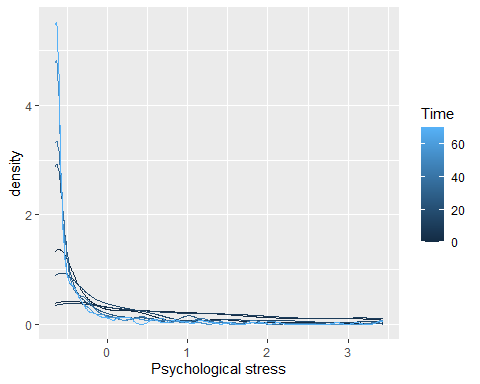
\includegraphics{01_Preprocessing_Modelling_files/figure-latex/wrap_res_stressed_2-1.pdf}

\begin{Shaded}
\begin{Highlighting}[]
\FunctionTok{ggplot}\NormalTok{(}\AttributeTok{data =}\NormalTok{ resall[[}\FunctionTok{paste0}\NormalTok{(depvar, }\StringTok{"\_longdat"}\NormalTok{)]], }
       \FunctionTok{aes}\NormalTok{(Time,DV, }\AttributeTok{col=}\NormalTok{group)) }\SpecialCharTok{+} 
  \FunctionTok{ylab}\NormalTok{(labeltag) }\SpecialCharTok{+} \FunctionTok{xlab}\NormalTok{(}\StringTok{"Time"}\NormalTok{)}\SpecialCharTok{+}
  \FunctionTok{geom\_smooth}\NormalTok{(}\AttributeTok{method =} \StringTok{\textquotesingle{}loess\textquotesingle{}}\NormalTok{) }\SpecialCharTok{+} \FunctionTok{geom\_point}\NormalTok{() }\SpecialCharTok{+}   \FunctionTok{facet\_wrap}\NormalTok{(}\SpecialCharTok{\textasciitilde{}}\NormalTok{gender)}
\end{Highlighting}
\end{Shaded}

\begin{verbatim}
## `geom_smooth()` using formula 'y ~ x'
\end{verbatim}

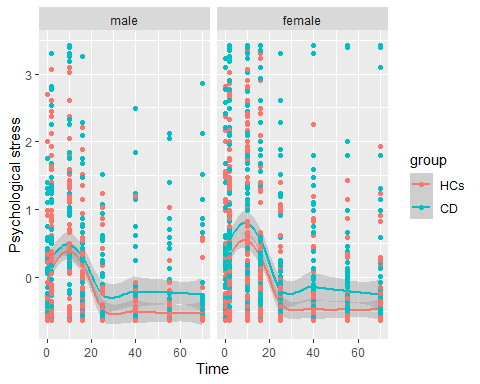
\includegraphics{01_Preprocessing_Modelling_files/figure-latex/wrap_res_stressed_2-2.pdf}

\hypertarget{sensitivity-analyses}{%
\paragraph{sensitivity analyses}\label{sensitivity-analyses}}

\begin{Shaded}
\begin{Highlighting}[]
\NormalTok{resall[[}\FunctionTok{paste0}\NormalTok{(depvar, }\StringTok{"\_coeff"}\NormalTok{)]] }\SpecialCharTok{\%\textgreater{}\%} \FunctionTok{tableplot}\NormalTok{()}
\end{Highlighting}
\end{Shaded}

\begin{table}
\centering
\begin{tabular}[t]{l|l|l|l|l}
\hline
  & Estimate & Std. Error & t value & pvalue\\
\hline
(Intercept) & -0.177 & 0.0846 & -2.09 & 0.0369\\
\hline
age\_meancentered & 0.0385 & 0.0373 & 1.03 & 0.301\\
\hline
genderfemale & 0.117 & 0.105 & 1.11 & 0.265\\
\hline
groupCD & 0.21 & 0.125 & 1.69 & 0.0915\\
\hline
poly(Time, 2)1 & -13.5 & 1.7 & -7.9 & 2.87e-15\\
\hline
poly(Time, 2)2 & 2.7 & 1.7 & 1.59 & 0.113\\
\hline
genderfemale:groupCD & 0.0258 & 0.156 & 0.165 & 0.869\\
\hline
groupCD:poly(Time, 2)1 & 2.65 & 2.51 & 1.06 & 0.291\\
\hline
groupCD:poly(Time, 2)2 & 0.0625 & 2.51 & 0.0249 & 0.98\\
\hline
genderfemale:poly(Time, 2)1 & -2.72 & 2.11 & -1.29 & 0.198\\
\hline
genderfemale:poly(Time, 2)2 & 1.71 & 2.11 & 0.807 & 0.42\\
\hline
genderfemale:groupCD:poly(Time, 2)1 & -2.1 & 3.14 & -0.67 & 0.503\\
\hline
genderfemale:groupCD:poly(Time, 2)2 & -1.28 & 3.14 & -0.408 & 0.683\\
\hline
\end{tabular}
\end{table}

\begin{Shaded}
\begin{Highlighting}[]
\NormalTok{resall[[}\FunctionTok{paste0}\NormalTok{(depvar, }\StringTok{"\_coeff\_CDquant"}\NormalTok{)]] }\SpecialCharTok{\%\textgreater{}\%} \FunctionTok{tableplot}\NormalTok{()}
\end{Highlighting}
\end{Shaded}

\begin{table}
\centering
\begin{tabular}[t]{l|l|l|l|l}
\hline
  & Estimate & Std. Error & t value & pvalue\\
\hline
(Intercept) & -0.0814 & 0.062 & -1.31 & 0.189\\
\hline
age\_meancentered & 0.0305 & 0.0373 & 0.817 & 0.414\\
\hline
genderfemale & 0.128 & 0.0775 & 1.66 & 0.0973\\
\hline
CDsymptomscurrent & 0.0603 & 0.0606 & 0.996 & 0.319\\
\hline
poly(Time, 2)1 & -12.3 & 1.25 & -9.82 & 8.86e-23\\
\hline
poly(Time, 2)2 & 2.73 & 1.25 & 2.18 & 0.0294\\
\hline
genderfemale:CDsymptomscurrent & 0.079 & 0.0767 & 1.03 & 0.303\\
\hline
CDsymptomscurrent:poly(Time, 2)1 & 1.7 & 1.22 & 1.39 & 0.165\\
\hline
CDsymptomscurrent:poly(Time, 2)2 & 0.253 & 1.22 & 0.207 & 0.836\\
\hline
genderfemale:poly(Time, 2)1 & -3.64 & 1.56 & -2.33 & 0.0197\\
\hline
genderfemale:poly(Time, 2)2 & 1.13 & 1.56 & 0.727 & 0.468\\
\hline
genderfemale:CDsymptomscurrent:poly(Time, 2)1 & -1.63 & 1.55 & -1.05 & 0.293\\
\hline
genderfemale:CDsymptomscurrent:poly(Time, 2)2 & -1.02 & 1.55 & -0.658 & 0.511\\
\hline
\end{tabular}
\end{table}

\begin{Shaded}
\begin{Highlighting}[]
\NormalTok{resall[[}\FunctionTok{paste0}\NormalTok{(depvar, }\StringTok{"\_coeff\_males"}\NormalTok{)]] }\SpecialCharTok{\%\textgreater{}\%} \FunctionTok{tableplot}\NormalTok{()}
\end{Highlighting}
\end{Shaded}

\begin{table}
\centering
\begin{tabular}[t]{l|l|l|l|l}
\hline
  & Estimate & Std. Error & t value & pvalue\\
\hline
(Intercept) & -0.172 & 0.0679 & -2.54 & 0.0111\\
\hline
age\_meancentered & -0.00906 & 0.0464 & -0.195 & 0.845\\
\hline
groupCD & 0.202 & 0.1 & 2.02 & 0.0433\\
\hline
poly(Time, 2)1 & -13.5 & 1.59 & -8.47 & 2.51e-17\\
\hline
poly(Time, 2)2 & 2.7 & 1.59 & 1.7 & 0.0888\\
\hline
groupCD:poly(Time, 2)1 & 2.65 & 2.34 & 1.13 & 0.257\\
\hline
groupCD:poly(Time, 2)2 & 0.0625 & 2.34 & 0.0267 & 0.979\\
\hline
\end{tabular}
\end{table}

\begin{Shaded}
\begin{Highlighting}[]
\NormalTok{resall[[}\FunctionTok{paste0}\NormalTok{(depvar, }\StringTok{"\_coeff\_females"}\NormalTok{)]] }\SpecialCharTok{\%\textgreater{}\%} \FunctionTok{tableplot}\NormalTok{()}
\end{Highlighting}
\end{Shaded}

\begin{table}
\centering
\begin{tabular}[t]{l|l|l|l|l}
\hline
  & Estimate & Std. Error & t value & pvalue\\
\hline
(Intercept) & -0.0575 & 0.068 & -0.846 & 0.398\\
\hline
age\_meancentered & 0.0722 & 0.0533 & 1.36 & 0.175\\
\hline
groupCD & 0.232 & 0.102 & 2.26 & 0.0237\\
\hline
poly(Time, 2)1 & -16.2 & 1.3 & -12.5 & 8.69e-36\\
\hline
poly(Time, 2)2 & 4.41 & 1.3 & 3.4 & 0.000662\\
\hline
groupCD:poly(Time, 2)1 & 0.55 & 1.95 & 0.282 & 0.778\\
\hline
groupCD:poly(Time, 2)2 & -1.22 & 1.95 & -0.624 & 0.532\\
\hline
\end{tabular}
\end{table}

\begin{Shaded}
\begin{Highlighting}[]
\NormalTok{resall[[}\FunctionTok{paste0}\NormalTok{(depvar, }\StringTok{"\_coeff\_iq\_e\_total\_imp\_meancentered"}\NormalTok{)]] }\SpecialCharTok{\%\textgreater{}\%} \FunctionTok{tableplot}\NormalTok{()}
\end{Highlighting}
\end{Shaded}

\begin{table}
\centering
\begin{tabular}[t]{l|l|l|l|l}
\hline
  & Estimate & Std. Error & t value & pvalue\\
\hline
(Intercept) & -0.179 & 0.0856 & -2.1 & 0.0361\\
\hline
iq\_e\_total\_imp\_meancentered & 0.00913 & 0.0394 & 0.232 & 0.817\\
\hline
age\_meancentered & 0.0403 & 0.0381 & 1.06 & 0.29\\
\hline
genderfemale & 0.118 & 0.105 & 1.12 & 0.262\\
\hline
groupCD & 0.214 & 0.126 & 1.7 & 0.089\\
\hline
poly(Time, 2)1 & -13.5 & 1.7 & -7.9 & 2.87e-15\\
\hline
poly(Time, 2)2 & 2.7 & 1.7 & 1.59 & 0.113\\
\hline
genderfemale:groupCD & 0.0271 & 0.156 & 0.173 & 0.863\\
\hline
groupCD:poly(Time, 2)1 & 2.65 & 2.51 & 1.06 & 0.291\\
\hline
groupCD:poly(Time, 2)2 & 0.0625 & 2.51 & 0.0249 & 0.98\\
\hline
genderfemale:poly(Time, 2)1 & -2.72 & 2.11 & -1.29 & 0.198\\
\hline
genderfemale:poly(Time, 2)2 & 1.71 & 2.11 & 0.807 & 0.42\\
\hline
genderfemale:groupCD:poly(Time, 2)1 & -2.1 & 3.14 & -0.67 & 0.503\\
\hline
genderfemale:groupCD:poly(Time, 2)2 & -1.28 & 3.14 & -0.408 & 0.683\\
\hline
\end{tabular}
\end{table}

\begin{Shaded}
\begin{Highlighting}[]
\NormalTok{resall[[}\FunctionTok{paste0}\NormalTok{(depvar, }\StringTok{"\_coeff\_EduParentsISCEDMean\_meancentered"}\NormalTok{)]] }\SpecialCharTok{\%\textgreater{}\%} \FunctionTok{tableplot}\NormalTok{()}
\end{Highlighting}
\end{Shaded}

\begin{table}
\centering
\begin{tabular}[t]{l|l|l|l|l}
\hline
  & Estimate & Std. Error & t value & pvalue\\
\hline
(Intercept) & -0.198 & 0.0899 & -2.2 & 0.0275\\
\hline
EduParentsISCEDMean\_meancentered & 0.0371 & 0.0431 & 0.861 & 0.389\\
\hline
age\_meancentered & 0.0178 & 0.0408 & 0.435 & 0.664\\
\hline
genderfemale & 0.118 & 0.112 & 1.05 & 0.292\\
\hline
groupCD & 0.287 & 0.135 & 2.13 & 0.0332\\
\hline
poly(Time, 2)1 & -12.4 & 1.78 & -6.97 & 3.23e-12\\
\hline
poly(Time, 2)2 & 2.74 & 1.78 & 1.54 & 0.124\\
\hline
genderfemale:groupCD & 0.00494 & 0.17 & 0.029 & 0.977\\
\hline
groupCD:poly(Time, 2)1 & 1.09 & 2.65 & 0.41 & 0.682\\
\hline
groupCD:poly(Time, 2)2 & 0.385 & 2.65 & 0.145 & 0.884\\
\hline
genderfemale:poly(Time, 2)1 & -3.56 & 2.22 & -1.61 & 0.108\\
\hline
genderfemale:poly(Time, 2)2 & 1.76 & 2.22 & 0.794 & 0.427\\
\hline
genderfemale:groupCD:poly(Time, 2)1 & -1.04 & 3.34 & -0.31 & 0.757\\
\hline
genderfemale:groupCD:poly(Time, 2)2 & -1.13 & 3.34 & -0.338 & 0.736\\
\hline
\end{tabular}
\end{table}

\begin{Shaded}
\begin{Highlighting}[]
\NormalTok{resall[[}\FunctionTok{paste0}\NormalTok{(depvar, }\StringTok{"\_coeff\_pubcatimp\_meancentered"}\NormalTok{)]] }\SpecialCharTok{\%\textgreater{}\%} \FunctionTok{tableplot}\NormalTok{()}
\end{Highlighting}
\end{Shaded}

\begin{table}
\centering
\begin{tabular}[t]{l|l|l|l|l}
\hline
  & Estimate & Std. Error & t value & pvalue\\
\hline
(Intercept) & -0.155 & 0.0928 & -1.67 & 0.0945\\
\hline
pubcatimp\_meancentered & 0.0323 & 0.0571 & 0.565 & 0.572\\
\hline
age\_meancentered & 0.0186 & 0.0513 & 0.363 & 0.717\\
\hline
genderfemale & 0.0852 & 0.119 & 0.714 & 0.475\\
\hline
groupCD & 0.206 & 0.125 & 1.64 & 0.1\\
\hline
poly(Time, 2)1 & -13.5 & 1.7 & -7.9 & 2.87e-15\\
\hline
poly(Time, 2)2 & 2.7 & 1.7 & 1.59 & 0.113\\
\hline
genderfemale:groupCD & 0.0297 & 0.156 & 0.19 & 0.85\\
\hline
groupCD:poly(Time, 2)1 & 2.65 & 2.51 & 1.06 & 0.291\\
\hline
groupCD:poly(Time, 2)2 & 0.0625 & 2.51 & 0.0249 & 0.98\\
\hline
genderfemale:poly(Time, 2)1 & -2.72 & 2.11 & -1.29 & 0.198\\
\hline
genderfemale:poly(Time, 2)2 & 1.71 & 2.11 & 0.807 & 0.42\\
\hline
genderfemale:groupCD:poly(Time, 2)1 & -2.1 & 3.14 & -0.67 & 0.503\\
\hline
genderfemale:groupCD:poly(Time, 2)2 & -1.28 & 3.14 & -0.408 & 0.683\\
\hline
\end{tabular}
\end{table}

\begin{Shaded}
\begin{Highlighting}[]
\NormalTok{resall[[}\FunctionTok{paste0}\NormalTok{(depvar, }\StringTok{"\_coeff\_ADHD\_life"}\NormalTok{)]] }\SpecialCharTok{\%\textgreater{}\%} \FunctionTok{tableplot}\NormalTok{()}
\end{Highlighting}
\end{Shaded}

\begin{table}
\centering
\begin{tabular}[t]{l|l|l|l|l}
\hline
  & Estimate & Std. Error & t value & pvalue\\
\hline
(Intercept) & -0.177 & 0.0847 & -2.09 & 0.0369\\
\hline
ADHD\_lifeADHD & 0.0734 & 0.114 & 0.642 & 0.521\\
\hline
age\_meancentered & 0.0409 & 0.0375 & 1.09 & 0.275\\
\hline
genderfemale & 0.117 & 0.105 & 1.12 & 0.264\\
\hline
groupCD & 0.168 & 0.141 & 1.19 & 0.234\\
\hline
poly(Time, 2)1 & -13.5 & 1.7 & -7.9 & 2.87e-15\\
\hline
poly(Time, 2)2 & 2.7 & 1.7 & 1.59 & 0.113\\
\hline
genderfemale:groupCD & 0.0402 & 0.158 & 0.255 & 0.799\\
\hline
groupCD:poly(Time, 2)1 & 2.65 & 2.51 & 1.06 & 0.291\\
\hline
groupCD:poly(Time, 2)2 & 0.0625 & 2.51 & 0.0249 & 0.98\\
\hline
genderfemale:poly(Time, 2)1 & -2.72 & 2.11 & -1.29 & 0.198\\
\hline
genderfemale:poly(Time, 2)2 & 1.71 & 2.11 & 0.807 & 0.42\\
\hline
genderfemale:groupCD:poly(Time, 2)1 & -2.1 & 3.14 & -0.67 & 0.503\\
\hline
genderfemale:groupCD:poly(Time, 2)2 & -1.28 & 3.14 & -0.408 & 0.683\\
\hline
\end{tabular}
\end{table}

\begin{Shaded}
\begin{Highlighting}[]
\NormalTok{resall[[}\FunctionTok{paste0}\NormalTok{(depvar, }\StringTok{"\_coeff\_Depression\_lifetime"}\NormalTok{)]] }\SpecialCharTok{\%\textgreater{}\%} \FunctionTok{tableplot}\NormalTok{()}
\end{Highlighting}
\end{Shaded}

\begin{table}
\centering
\begin{tabular}[t]{l|l|l|l|l}
\hline
  & Estimate & Std. Error & t value & pvalue\\
\hline
(Intercept) & -0.177 & 0.084 & -2.11 & 0.0351\\
\hline
Depression\_lifetimeDepression & 0.253 & 0.113 & 2.24 & 0.0248\\
\hline
age\_meancentered & 0.0441 & 0.0371 & 1.19 & 0.235\\
\hline
genderfemale & 0.108 & 0.104 & 1.04 & 0.3\\
\hline
groupCD & 0.164 & 0.125 & 1.31 & 0.192\\
\hline
poly(Time, 2)1 & -13.5 & 1.7 & -7.9 & 2.87e-15\\
\hline
poly(Time, 2)2 & 2.7 & 1.7 & 1.59 & 0.113\\
\hline
genderfemale:groupCD & -0.0267 & 0.157 & -0.17 & 0.865\\
\hline
groupCD:poly(Time, 2)1 & 2.65 & 2.51 & 1.06 & 0.291\\
\hline
groupCD:poly(Time, 2)2 & 0.0625 & 2.51 & 0.0249 & 0.98\\
\hline
genderfemale:poly(Time, 2)1 & -2.72 & 2.11 & -1.29 & 0.198\\
\hline
genderfemale:poly(Time, 2)2 & 1.71 & 2.11 & 0.807 & 0.42\\
\hline
genderfemale:groupCD:poly(Time, 2)1 & -2.1 & 3.14 & -0.67 & 0.503\\
\hline
genderfemale:groupCD:poly(Time, 2)2 & -1.28 & 3.14 & -0.408 & 0.683\\
\hline
\end{tabular}
\end{table}

\begin{Shaded}
\begin{Highlighting}[]
\NormalTok{resall[[}\FunctionTok{paste0}\NormalTok{(depvar, }\StringTok{"\_coeff\_PTSD\_lifetime"}\NormalTok{)]] }\SpecialCharTok{\%\textgreater{}\%} \FunctionTok{tableplot}\NormalTok{()}
\end{Highlighting}
\end{Shaded}

\begin{table}
\centering
\begin{tabular}[t]{l|l|l|l|l}
\hline
  & Estimate & Std. Error & t value & pvalue\\
\hline
(Intercept) & -0.185 & 0.0835 & -2.22 & 0.0266\\
\hline
PTSD\_lifetimePTSD & 0.476 & 0.156 & 3.05 & 0.00229\\
\hline
age\_meancentered & 0.0379 & 0.0367 & 1.03 & 0.302\\
\hline
genderfemale & 0.121 & 0.104 & 1.17 & 0.243\\
\hline
groupCD & 0.169 & 0.124 & 1.37 & 0.171\\
\hline
poly(Time, 2)1 & -13.5 & 1.7 & -7.9 & 2.87e-15\\
\hline
poly(Time, 2)2 & 2.7 & 1.7 & 1.59 & 0.113\\
\hline
genderfemale:groupCD & 0.00782 & 0.154 & 0.0508 & 0.96\\
\hline
groupCD:poly(Time, 2)1 & 2.65 & 2.51 & 1.06 & 0.291\\
\hline
groupCD:poly(Time, 2)2 & 0.0625 & 2.51 & 0.0249 & 0.98\\
\hline
genderfemale:poly(Time, 2)1 & -2.72 & 2.11 & -1.29 & 0.198\\
\hline
genderfemale:poly(Time, 2)2 & 1.71 & 2.11 & 0.807 & 0.42\\
\hline
genderfemale:groupCD:poly(Time, 2)1 & -2.1 & 3.14 & -0.67 & 0.503\\
\hline
genderfemale:groupCD:poly(Time, 2)2 & -1.28 & 3.14 & -0.408 & 0.683\\
\hline
\end{tabular}
\end{table}

\begin{Shaded}
\begin{Highlighting}[]
\NormalTok{resall[[}\FunctionTok{paste0}\NormalTok{(depvar, }\StringTok{"\_coeff\_SUD\_life"}\NormalTok{)]] }\SpecialCharTok{\%\textgreater{}\%} \FunctionTok{tableplot}\NormalTok{()}
\end{Highlighting}
\end{Shaded}

\begin{table}
\centering
\begin{tabular}[t]{l|l|l|l|l}
\hline
  & Estimate & Std. Error & t value & pvalue\\
\hline
(Intercept) & -0.179 & 0.0844 & -2.12 & 0.0337\\
\hline
SUD\_lifeSUD & 0.211 & 0.129 & 1.64 & 0.102\\
\hline
age\_meancentered & 0.0262 & 0.0379 & 0.691 & 0.489\\
\hline
genderfemale & 0.119 & 0.105 & 1.13 & 0.256\\
\hline
groupCD & 0.151 & 0.13 & 1.16 & 0.245\\
\hline
poly(Time, 2)1 & -13.5 & 1.7 & -7.9 & 2.87e-15\\
\hline
poly(Time, 2)2 & 2.7 & 1.7 & 1.59 & 0.113\\
\hline
genderfemale:groupCD & 0.041 & 0.156 & 0.263 & 0.793\\
\hline
groupCD:poly(Time, 2)1 & 2.65 & 2.51 & 1.06 & 0.291\\
\hline
groupCD:poly(Time, 2)2 & 0.0625 & 2.51 & 0.0249 & 0.98\\
\hline
genderfemale:poly(Time, 2)1 & -2.72 & 2.11 & -1.29 & 0.198\\
\hline
genderfemale:poly(Time, 2)2 & 1.71 & 2.11 & 0.807 & 0.42\\
\hline
genderfemale:groupCD:poly(Time, 2)1 & -2.1 & 3.14 & -0.67 & 0.503\\
\hline
genderfemale:groupCD:poly(Time, 2)2 & -1.28 & 3.14 & -0.408 & 0.683\\
\hline
\end{tabular}
\end{table}

\begin{Shaded}
\begin{Highlighting}[]
\NormalTok{resall[[}\FunctionTok{paste0}\NormalTok{(depvar, }\StringTok{"\_coeff\_Anxiety\_lifetime"}\NormalTok{)]] }\SpecialCharTok{\%\textgreater{}\%} \FunctionTok{tableplot}\NormalTok{()}
\end{Highlighting}
\end{Shaded}

\begin{table}
\centering
\begin{tabular}[t]{l|l|l|l|l}
\hline
  & Estimate & Std. Error & t value & pvalue\\
\hline
(Intercept) & -0.191 & 0.0833 & -2.3 & 0.0216\\
\hline
Anxiety\_lifetimeAnxiety & 0.386 & 0.116 & 3.33 & 0.000872\\
\hline
age\_meancentered & 0.0489 & 0.0368 & 1.33 & 0.183\\
\hline
genderfemale & 0.125 & 0.103 & 1.21 & 0.226\\
\hline
groupCD & 0.0891 & 0.128 & 0.697 & 0.486\\
\hline
poly(Time, 2)1 & -13.5 & 1.7 & -7.9 & 2.87e-15\\
\hline
poly(Time, 2)2 & 2.7 & 1.7 & 1.59 & 0.113\\
\hline
genderfemale:groupCD & 0.0683 & 0.154 & 0.444 & 0.657\\
\hline
groupCD:poly(Time, 2)1 & 2.65 & 2.51 & 1.06 & 0.291\\
\hline
groupCD:poly(Time, 2)2 & 0.0625 & 2.51 & 0.0249 & 0.98\\
\hline
genderfemale:poly(Time, 2)1 & -2.72 & 2.11 & -1.29 & 0.198\\
\hline
genderfemale:poly(Time, 2)2 & 1.71 & 2.11 & 0.807 & 0.42\\
\hline
genderfemale:groupCD:poly(Time, 2)1 & -2.1 & 3.14 & -0.67 & 0.503\\
\hline
genderfemale:groupCD:poly(Time, 2)2 & -1.28 & 3.14 & -0.408 & 0.683\\
\hline
\end{tabular}
\end{table}

\hypertarget{cort}{%
\subsubsection{CORT}\label{cort}}

full models:
DV\textasciitilde1+age\_meancentered+explstart\_meancentered\_min+BMI\_imp\_meancentered+any\_med\_ccept+smoking\_yes\_no+gender+group+poly(Time,
2)+gender\emph{group+poly(Time, 2)}group+gender\emph{poly(Time,
2)}group+(1\textbar twuid)+(1\textbar centre)

h0 model:DV\textasciitilde1+(1\textbar twuid)+(1\textbar centre):

overall model p-value:9.94e-62

\begin{Shaded}
\begin{Highlighting}[]
\NormalTok{depvar }\OtherTok{=} \StringTok{"AV\_CORT"}
\NormalTok{labeltag }\OtherTok{=} \StringTok{"Cortisol"}

\FunctionTok{ggplot}\NormalTok{(}\AttributeTok{data =}\NormalTok{ resall[[}\FunctionTok{paste0}\NormalTok{(depvar, }\StringTok{"\_longdat"}\NormalTok{)]], }
       \FunctionTok{aes}\NormalTok{(DV, }\AttributeTok{group=}\NormalTok{Time, }\AttributeTok{col=}\NormalTok{Time)) }\SpecialCharTok{+} 
  \FunctionTok{ylab}\NormalTok{(}\StringTok{"density"}\NormalTok{) }\SpecialCharTok{+} \FunctionTok{xlab}\NormalTok{(labeltag)}\SpecialCharTok{+}
  \FunctionTok{geom\_density}\NormalTok{()}
\end{Highlighting}
\end{Shaded}

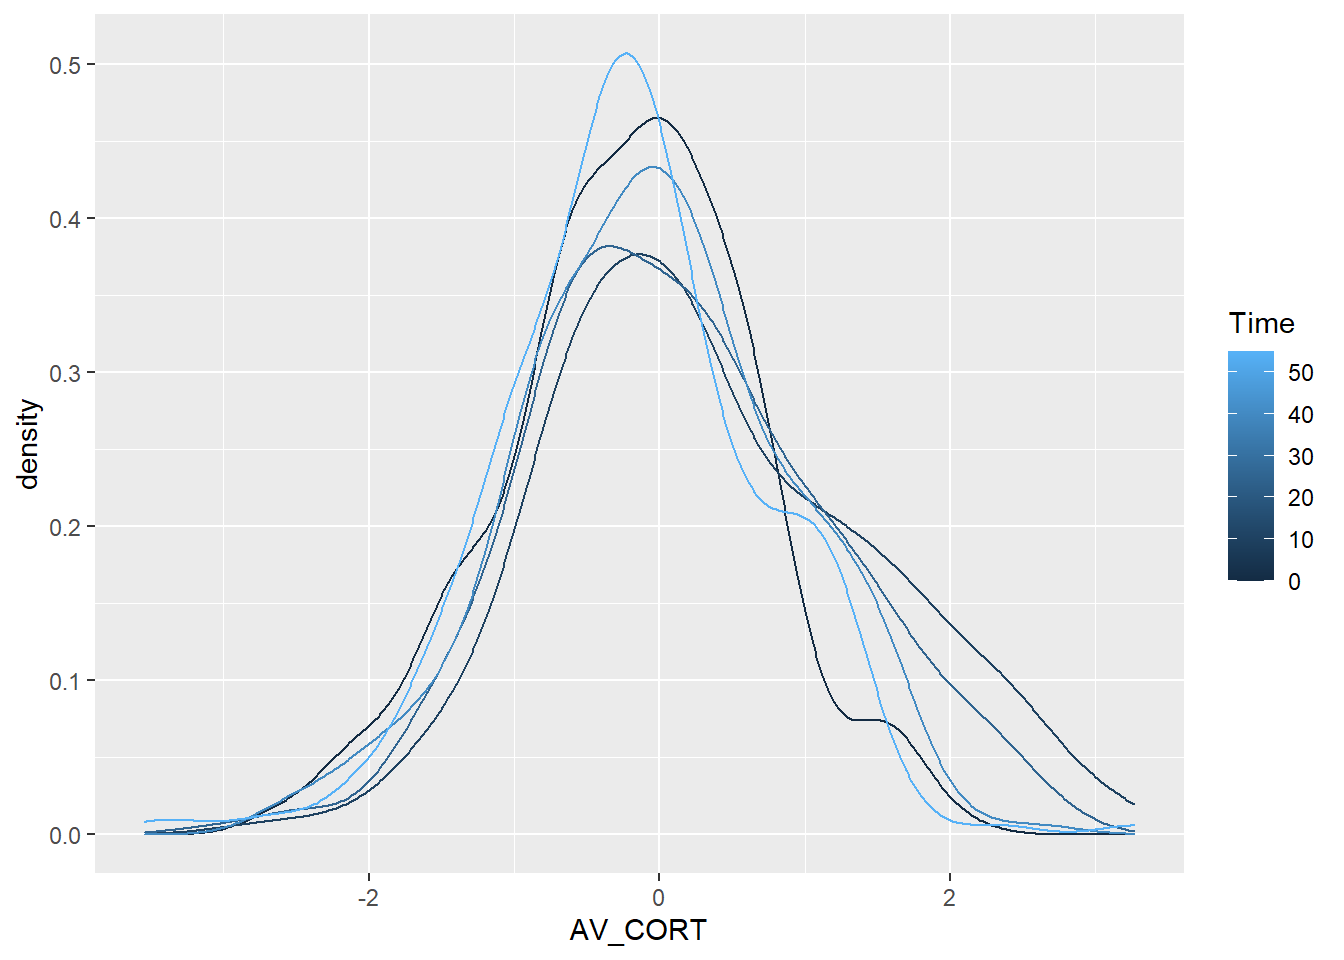
\includegraphics{01_Preprocessing_Modelling_files/figure-latex/wrap_res_CORT_2-1.pdf}

\begin{Shaded}
\begin{Highlighting}[]
\FunctionTok{ggplot}\NormalTok{(}\AttributeTok{data =}\NormalTok{ resall[[}\FunctionTok{paste0}\NormalTok{(depvar, }\StringTok{"\_longdat"}\NormalTok{)]], }
       \FunctionTok{aes}\NormalTok{(Time,DV, }\AttributeTok{col=}\NormalTok{group)) }\SpecialCharTok{+} 
  \FunctionTok{ylab}\NormalTok{(labeltag) }\SpecialCharTok{+} \FunctionTok{xlab}\NormalTok{(}\StringTok{"Time"}\NormalTok{)}\SpecialCharTok{+}
  \FunctionTok{geom\_smooth}\NormalTok{(}\AttributeTok{method =} \StringTok{\textquotesingle{}loess\textquotesingle{}}\NormalTok{) }\SpecialCharTok{+} \FunctionTok{geom\_point}\NormalTok{() }\SpecialCharTok{+}   \FunctionTok{facet\_wrap}\NormalTok{(}\SpecialCharTok{\textasciitilde{}}\NormalTok{gender)}
\end{Highlighting}
\end{Shaded}

\begin{verbatim}
## `geom_smooth()` using formula 'y ~ x'
\end{verbatim}

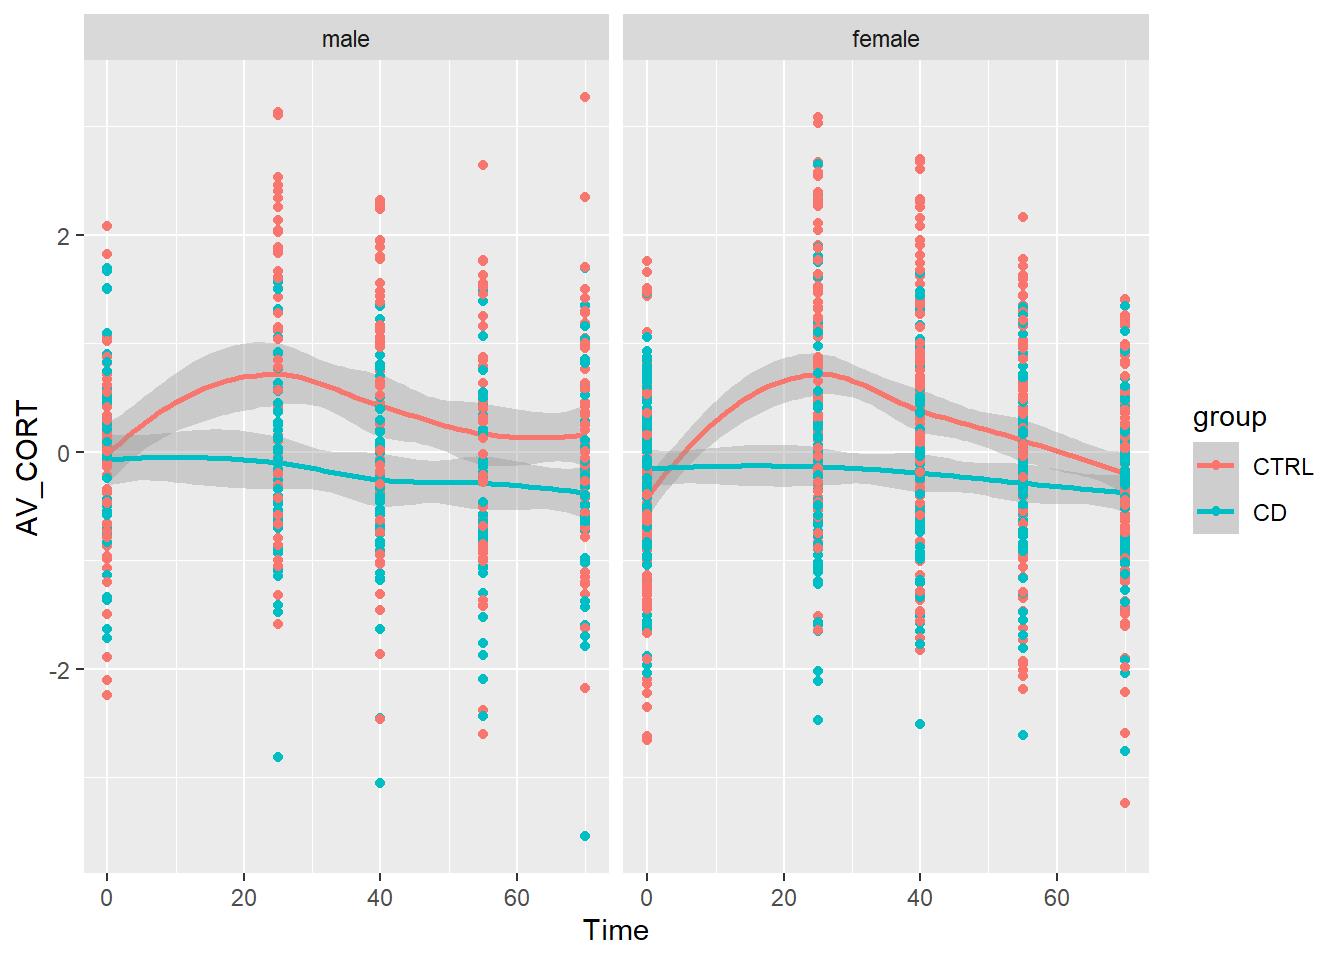
\includegraphics{01_Preprocessing_Modelling_files/figure-latex/wrap_res_CORT_2-2.pdf}

\hypertarget{sensitivity-analyses-1}{%
\paragraph{sensitivity analyses}\label{sensitivity-analyses-1}}

\begin{Shaded}
\begin{Highlighting}[]
\NormalTok{resall[[}\FunctionTok{paste0}\NormalTok{(depvar, }\StringTok{"\_coeff"}\NormalTok{)]] }\SpecialCharTok{\%\textgreater{}\%} \FunctionTok{tableplot}\NormalTok{()}
\end{Highlighting}
\end{Shaded}

\begin{table}
\centering
\begin{tabular}[t]{l|l|l|l|l}
\hline
  & Estimate & Std. Error & t value & pvalue\\
\hline
(Intercept) & 0.24 & 0.112 & 2.14 & 0.0322\\
\hline
age\_meancentered & 0.239 & 0.0513 & 4.65 & 3.25e-06\\
\hline
explstart\_meancentered\_min & -0.177 & 0.0461 & -3.85 & 0.000116\\
\hline
BMI\_imp\_meancentered & 0.049 & 0.0473 & 1.04 & 0.301\\
\hline
any\_med\_cceptmed & -0.021 & 0.122 & -0.172 & 0.863\\
\hline
smoking\_yes\_nosmk & -0.106 & 0.125 & -0.846 & 0.397\\
\hline
genderfemale & -0.0705 & 0.129 & -0.546 & 0.585\\
\hline
groupCD & -0.415 & 0.16 & -2.6 & 0.00939\\
\hline
poly(Time, 2)1 & 0.0446 & 1.23 & 0.0361 & 0.971\\
\hline
poly(Time, 2)2 & -7.78 & 1.23 & -6.31 & 2.81e-10\\
\hline
genderfemale:groupCD & 0.0515 & 0.194 & 0.266 & 0.791\\
\hline
groupCD:poly(Time, 2)1 & -4.25 & 1.82 & -2.34 & 0.0191\\
\hline
groupCD:poly(Time, 2)2 & 7.25 & 1.82 & 4 & 6.46e-05\\
\hline
genderfemale:poly(Time, 2)1 & 0.948 & 1.53 & 0.62 & 0.536\\
\hline
genderfemale:poly(Time, 2)2 & -6.3 & 1.53 & -4.12 & 3.78e-05\\
\hline
genderfemale:groupCD:poly(Time, 2)1 & 0.241 & 2.27 & 0.106 & 0.915\\
\hline
genderfemale:groupCD:poly(Time, 2)2 & 5.3 & 2.27 & 2.34 & 0.0195\\
\hline
\end{tabular}
\end{table}

\begin{Shaded}
\begin{Highlighting}[]
\NormalTok{resall[[}\FunctionTok{paste0}\NormalTok{(depvar, }\StringTok{"\_coeff\_CDquant"}\NormalTok{)]] }\SpecialCharTok{\%\textgreater{}\%} \FunctionTok{tableplot}\NormalTok{()}
\end{Highlighting}
\end{Shaded}

\begin{table}
\centering
\begin{tabular}[t]{l|l|l|l|l}
\hline
  & Estimate & Std. Error & t value & pvalue\\
\hline
(Intercept) & 0.0779 & 0.0945 & 0.824 & 0.41\\
\hline
age\_meancentered & 0.259 & 0.0507 & 5.12 & 3.07e-07\\
\hline
explstart\_meancentered\_min & -0.172 & 0.0463 & -3.73 & 0.000195\\
\hline
BMI\_imp\_meancentered & 0.0352 & 0.0472 & 0.747 & 0.455\\
\hline
any\_med\_cceptmed & -0.0485 & 0.121 & -0.401 & 0.689\\
\hline
smoking\_yes\_nosmk & -0.155 & 0.128 & -1.21 & 0.226\\
\hline
genderfemale & -0.0438 & 0.0995 & -0.44 & 0.66\\
\hline
CDsymptomscurrent & -0.103 & 0.0802 & -1.28 & 0.2\\
\hline
poly(Time, 2)1 & -1.85 & 0.919 & -2.02 & 0.0436\\
\hline
poly(Time, 2)2 & -4.53 & 0.919 & -4.92 & 8.48e-07\\
\hline
genderfemale:CDsymptomscurrent & -0.0525 & 0.0947 & -0.554 & 0.579\\
\hline
CDsymptomscurrent:poly(Time, 2)1 & -1.96 & 0.897 & -2.19 & 0.0288\\
\hline
CDsymptomscurrent:poly(Time, 2)2 & 2.79 & 0.897 & 3.11 & 0.00189\\
\hline
genderfemale:poly(Time, 2)1 & 1.05 & 1.15 & 0.913 & 0.361\\
\hline
genderfemale:poly(Time, 2)2 & -3.93 & 1.15 & -3.42 & 0.000619\\
\hline
genderfemale:CDsymptomscurrent:poly(Time, 2)1 & 0.344 & 1.14 & 0.302 & 0.762\\
\hline
genderfemale:CDsymptomscurrent:poly(Time, 2)2 & 2.52 & 1.14 & 2.22 & 0.0264\\
\hline
\end{tabular}
\end{table}

\begin{Shaded}
\begin{Highlighting}[]
\NormalTok{resall[[}\FunctionTok{paste0}\NormalTok{(depvar, }\StringTok{"\_coeff\_males"}\NormalTok{)]] }\SpecialCharTok{\%\textgreater{}\%} \FunctionTok{tableplot}\NormalTok{()}
\end{Highlighting}
\end{Shaded}

\begin{table}
\centering
\begin{tabular}[t]{l|l|l|l|l}
\hline
  & Estimate & Std. Error & t value & pvalue\\
\hline
(Intercept) & 0.245 & 0.114 & 2.16 & 0.0307\\
\hline
age\_meancentered & 0.26 & 0.0964 & 2.7 & 0.0069\\
\hline
explstart\_meancentered\_min & -0.259 & 0.0873 & -2.96 & 0.00304\\
\hline
BMI\_imp\_meancentered & 0.0898 & 0.107 & 0.842 & 0.4\\
\hline
any\_med\_cceptmed & 0.116 & 0.261 & 0.443 & 0.658\\
\hline
smoking\_yes\_nosmk & -0.129 & 0.219 & -0.593 & 0.553\\
\hline
groupCD & -0.411 & 0.18 & -2.28 & 0.0227\\
\hline
poly(Time, 2)1 & 0.0446 & 1.17 & 0.0381 & 0.97\\
\hline
poly(Time, 2)2 & -7.78 & 1.17 & -6.65 & 2.95e-11\\
\hline
groupCD:poly(Time, 2)1 & -4.25 & 1.72 & -2.47 & 0.0135\\
\hline
groupCD:poly(Time, 2)2 & 7.25 & 1.72 & 4.21 & 2.55e-05\\
\hline
\end{tabular}
\end{table}

\begin{Shaded}
\begin{Highlighting}[]
\NormalTok{resall[[}\FunctionTok{paste0}\NormalTok{(depvar, }\StringTok{"\_coeff\_females"}\NormalTok{)]] }\SpecialCharTok{\%\textgreater{}\%} \FunctionTok{tableplot}\NormalTok{()}
\end{Highlighting}
\end{Shaded}

\begin{table}
\centering
\begin{tabular}[t]{l|l|l|l|l}
\hline
  & Estimate & Std. Error & t value & pvalue\\
\hline
(Intercept) & 0.148 & 0.099 & 1.5 & 0.135\\
\hline
age\_meancentered & 0.221 & 0.0639 & 3.46 & 0.000535\\
\hline
explstart\_meancentered\_min & -0.132 & 0.0543 & -2.44 & 0.0148\\
\hline
BMI\_imp\_meancentered & 0.0345 & 0.0524 & 0.658 & 0.511\\
\hline
any\_med\_cceptmed & -0.0576 & 0.142 & -0.407 & 0.684\\
\hline
smoking\_yes\_nosmk & -0.119 & 0.157 & -0.754 & 0.451\\
\hline
groupCD & -0.317 & 0.16 & -1.99 & 0.0469\\
\hline
poly(Time, 2)1 & 0.992 & 0.93 & 1.07 & 0.286\\
\hline
poly(Time, 2)2 & -14.1 & 0.93 & -15.1 & 7.82e-52\\
\hline
groupCD:poly(Time, 2)1 & -4.01 & 1.4 & -2.87 & 0.00416\\
\hline
groupCD:poly(Time, 2)2 & 12.6 & 1.4 & 8.96 & 3.11e-19\\
\hline
\end{tabular}
\end{table}

\begin{Shaded}
\begin{Highlighting}[]
\NormalTok{resall[[}\FunctionTok{paste0}\NormalTok{(depvar, }\StringTok{"\_coeff\_iq\_e\_total\_imp\_meancentered"}\NormalTok{)]] }\SpecialCharTok{\%\textgreater{}\%} \FunctionTok{tableplot}\NormalTok{()}
\end{Highlighting}
\end{Shaded}

\begin{table}
\centering
\begin{tabular}[t]{l|l|l|l|l}
\hline
  & Estimate & Std. Error & t value & pvalue\\
\hline
(Intercept) & 0.245 & 0.115 & 2.13 & 0.0329\\
\hline
iq\_e\_total\_imp\_meancentered & -0.0331 & 0.0482 & -0.687 & 0.492\\
\hline
age\_meancentered & 0.235 & 0.0519 & 4.54 & 5.74e-06\\
\hline
explstart\_meancentered\_min & -0.179 & 0.0461 & -3.88 & 0.000106\\
\hline
BMI\_imp\_meancentered & 0.0463 & 0.0474 & 0.975 & 0.329\\
\hline
any\_med\_cceptmed & -0.025 & 0.122 & -0.205 & 0.838\\
\hline
smoking\_yes\_nosmk & -0.11 & 0.126 & -0.875 & 0.382\\
\hline
genderfemale & -0.0726 & 0.129 & -0.56 & 0.575\\
\hline
groupCD & -0.426 & 0.16 & -2.66 & 0.00786\\
\hline
poly(Time, 2)1 & 0.0446 & 1.23 & 0.0361 & 0.971\\
\hline
poly(Time, 2)2 & -7.78 & 1.23 & -6.31 & 2.81e-10\\
\hline
genderfemale:groupCD & 0.0523 & 0.194 & 0.269 & 0.788\\
\hline
groupCD:poly(Time, 2)1 & -4.25 & 1.82 & -2.34 & 0.0191\\
\hline
groupCD:poly(Time, 2)2 & 7.25 & 1.82 & 4 & 6.46e-05\\
\hline
genderfemale:poly(Time, 2)1 & 0.948 & 1.53 & 0.62 & 0.536\\
\hline
genderfemale:poly(Time, 2)2 & -6.3 & 1.53 & -4.12 & 3.78e-05\\
\hline
genderfemale:groupCD:poly(Time, 2)1 & 0.241 & 2.27 & 0.106 & 0.915\\
\hline
genderfemale:groupCD:poly(Time, 2)2 & 5.3 & 2.27 & 2.34 & 0.0195\\
\hline
\end{tabular}
\end{table}

\begin{Shaded}
\begin{Highlighting}[]
\NormalTok{resall[[}\FunctionTok{paste0}\NormalTok{(depvar, }\StringTok{"\_coeff\_EduParentsISCEDMean\_meancentered"}\NormalTok{)]] }\SpecialCharTok{\%\textgreater{}\%} \FunctionTok{tableplot}\NormalTok{()}
\end{Highlighting}
\end{Shaded}

\begin{table}
\centering
\begin{tabular}[t]{l|l|l|l|l}
\hline
  & Estimate & Std. Error & t value & pvalue\\
\hline
(Intercept) & 0.244 & 0.121 & 2.02 & 0.0438\\
\hline
EduParentsISCEDMean\_meancentered & -0.0159 & 0.0524 & -0.304 & 0.761\\
\hline
age\_meancentered & 0.253 & 0.0556 & 4.54 & 5.57e-06\\
\hline
explstart\_meancentered\_min & -0.177 & 0.0541 & -3.27 & 0.00106\\
\hline
BMI\_imp\_meancentered & 0.0606 & 0.0587 & 1.03 & 0.302\\
\hline
any\_med\_cceptmed & 0.0315 & 0.132 & 0.238 & 0.812\\
\hline
smoking\_yes\_nosmk & -0.166 & 0.135 & -1.23 & 0.219\\
\hline
genderfemale & -0.053 & 0.138 & -0.384 & 0.701\\
\hline
groupCD & -0.421 & 0.171 & -2.46 & 0.014\\
\hline
poly(Time, 2)1 & 0.0738 & 1.29 & 0.0571 & 0.954\\
\hline
poly(Time, 2)2 & -7.14 & 1.29 & -5.52 & 3.39e-08\\
\hline
genderfemale:groupCD & 0.0329 & 0.213 & 0.155 & 0.877\\
\hline
groupCD:poly(Time, 2)1 & -4.92 & 1.92 & -2.56 & 0.0106\\
\hline
groupCD:poly(Time, 2)2 & 5.39 & 1.92 & 2.8 & 0.00509\\
\hline
genderfemale:poly(Time, 2)1 & 1.29 & 1.61 & 0.802 & 0.422\\
\hline
genderfemale:poly(Time, 2)2 & -6.48 & 1.61 & -4.02 & 5.82e-05\\
\hline
genderfemale:groupCD:poly(Time, 2)1 & 0.441 & 2.43 & 0.182 & 0.856\\
\hline
genderfemale:groupCD:poly(Time, 2)2 & 6.29 & 2.43 & 2.59 & 0.0095\\
\hline
\end{tabular}
\end{table}

\begin{Shaded}
\begin{Highlighting}[]
\NormalTok{resall[[}\FunctionTok{paste0}\NormalTok{(depvar, }\StringTok{"\_coeff\_pubcatimp\_meancentered"}\NormalTok{)]] }\SpecialCharTok{\%\textgreater{}\%} \FunctionTok{tableplot}\NormalTok{()}
\end{Highlighting}
\end{Shaded}

\begin{table}
\centering
\begin{tabular}[t]{l|l|l|l|l}
\hline
  & Estimate & Std. Error & t value & pvalue\\
\hline
(Intercept) & 0.333 & 0.125 & 2.66 & 0.0078\\
\hline
pubcatimp\_meancentered & 0.158 & 0.0699 & 2.26 & 0.0236\\
\hline
age\_meancentered & 0.154 & 0.0642 & 2.4 & 0.0162\\
\hline
explstart\_meancentered\_min & -0.174 & 0.0459 & -3.79 & 0.000152\\
\hline
BMI\_imp\_meancentered & 0.0315 & 0.0475 & 0.663 & 0.507\\
\hline
any\_med\_cceptmed & -0.0622 & 0.122 & -0.51 & 0.61\\
\hline
smoking\_yes\_nosmk & -0.119 & 0.125 & -0.955 & 0.34\\
\hline
genderfemale & -0.22 & 0.146 & -1.51 & 0.131\\
\hline
groupCD & -0.428 & 0.158 & -2.7 & 0.00697\\
\hline
poly(Time, 2)1 & 0.0446 & 1.23 & 0.0361 & 0.971\\
\hline
poly(Time, 2)2 & -7.78 & 1.23 & -6.31 & 2.81e-10\\
\hline
genderfemale:groupCD & 0.0984 & 0.194 & 0.508 & 0.612\\
\hline
groupCD:poly(Time, 2)1 & -4.25 & 1.82 & -2.34 & 0.0191\\
\hline
groupCD:poly(Time, 2)2 & 7.25 & 1.82 & 4 & 6.46e-05\\
\hline
genderfemale:poly(Time, 2)1 & 0.948 & 1.53 & 0.62 & 0.536\\
\hline
genderfemale:poly(Time, 2)2 & -6.3 & 1.53 & -4.12 & 3.78e-05\\
\hline
genderfemale:groupCD:poly(Time, 2)1 & 0.241 & 2.27 & 0.106 & 0.915\\
\hline
genderfemale:groupCD:poly(Time, 2)2 & 5.3 & 2.27 & 2.34 & 0.0195\\
\hline
\end{tabular}
\end{table}

\begin{Shaded}
\begin{Highlighting}[]
\NormalTok{resall[[}\FunctionTok{paste0}\NormalTok{(depvar, }\StringTok{"\_coeff\_ADHD\_life"}\NormalTok{)]] }\SpecialCharTok{\%\textgreater{}\%} \FunctionTok{tableplot}\NormalTok{()}
\end{Highlighting}
\end{Shaded}

\begin{table}
\centering
\begin{tabular}[t]{l|l|l|l|l}
\hline
  & Estimate & Std. Error & t value & pvalue\\
\hline
(Intercept) & 0.24 & 0.114 & 2.11 & 0.0346\\
\hline
ADHD\_lifeADHD & -0.118 & 0.14 & -0.846 & 0.398\\
\hline
age\_meancentered & 0.238 & 0.0515 & 4.63 & 3.65e-06\\
\hline
explstart\_meancentered\_min & -0.177 & 0.0461 & -3.83 & 0.000127\\
\hline
BMI\_imp\_meancentered & 0.0512 & 0.0474 & 1.08 & 0.28\\
\hline
any\_med\_cceptmed & -0.0262 & 0.122 & -0.215 & 0.83\\
\hline
smoking\_yes\_nosmk & -0.118 & 0.126 & -0.934 & 0.35\\
\hline
genderfemale & -0.0698 & 0.129 & -0.54 & 0.589\\
\hline
groupCD & -0.343 & 0.181 & -1.89 & 0.0588\\
\hline
poly(Time, 2)1 & 0.0446 & 1.23 & 0.0361 & 0.971\\
\hline
poly(Time, 2)2 & -7.78 & 1.23 & -6.31 & 2.81e-10\\
\hline
genderfemale:groupCD & 0.0322 & 0.196 & 0.164 & 0.87\\
\hline
groupCD:poly(Time, 2)1 & -4.25 & 1.82 & -2.34 & 0.0191\\
\hline
groupCD:poly(Time, 2)2 & 7.25 & 1.82 & 4 & 6.46e-05\\
\hline
genderfemale:poly(Time, 2)1 & 0.948 & 1.53 & 0.62 & 0.536\\
\hline
genderfemale:poly(Time, 2)2 & -6.3 & 1.53 & -4.12 & 3.78e-05\\
\hline
genderfemale:groupCD:poly(Time, 2)1 & 0.241 & 2.27 & 0.106 & 0.915\\
\hline
genderfemale:groupCD:poly(Time, 2)2 & 5.3 & 2.27 & 2.34 & 0.0195\\
\hline
\end{tabular}
\end{table}

\begin{Shaded}
\begin{Highlighting}[]
\NormalTok{resall[[}\FunctionTok{paste0}\NormalTok{(depvar, }\StringTok{"\_coeff\_Depression\_lifetime"}\NormalTok{)]] }\SpecialCharTok{\%\textgreater{}\%} \FunctionTok{tableplot}\NormalTok{()}
\end{Highlighting}
\end{Shaded}

\begin{table}
\centering
\begin{tabular}[t]{l|l|l|l|l}
\hline
  & Estimate & Std. Error & t value & pvalue\\
\hline
(Intercept) & 0.263 & 0.105 & 2.51 & 0.0121\\
\hline
Depression\_lifetimeDepression & 0.0505 & 0.141 & 0.359 & 0.72\\
\hline
age\_meancentered & 0.234 & 0.051 & 4.58 & 4.71e-06\\
\hline
explstart\_meancentered\_min & -0.173 & 0.046 & -3.76 & 0.000169\\
\hline
BMI\_imp\_meancentered & 0.0535 & 0.0476 & 1.12 & 0.262\\
\hline
any\_med\_cceptmed & -0.011 & 0.123 & -0.0895 & 0.929\\
\hline
smoking\_yes\_nosmk & -0.123 & 0.125 & -0.979 & 0.328\\
\hline
genderfemale & -0.084 & 0.129 & -0.653 & 0.514\\
\hline
groupCD & -0.412 & 0.161 & -2.56 & 0.0104\\
\hline
poly(Time, 2)1 & 0.0446 & 1.23 & 0.0361 & 0.971\\
\hline
poly(Time, 2)2 & -7.78 & 1.23 & -6.31 & 2.81e-10\\
\hline
genderfemale:groupCD & 0.0303 & 0.195 & 0.155 & 0.877\\
\hline
groupCD:poly(Time, 2)1 & -4.25 & 1.82 & -2.34 & 0.0191\\
\hline
groupCD:poly(Time, 2)2 & 7.25 & 1.82 & 4 & 6.46e-05\\
\hline
genderfemale:poly(Time, 2)1 & 0.948 & 1.53 & 0.62 & 0.536\\
\hline
genderfemale:poly(Time, 2)2 & -6.3 & 1.53 & -4.12 & 3.78e-05\\
\hline
genderfemale:groupCD:poly(Time, 2)1 & 0.241 & 2.27 & 0.106 & 0.915\\
\hline
genderfemale:groupCD:poly(Time, 2)2 & 5.3 & 2.27 & 2.34 & 0.0195\\
\hline
\end{tabular}
\end{table}

\begin{Shaded}
\begin{Highlighting}[]
\NormalTok{resall[[}\FunctionTok{paste0}\NormalTok{(depvar, }\StringTok{"\_coeff\_PTSD\_lifetime"}\NormalTok{)]] }\SpecialCharTok{\%\textgreater{}\%} \FunctionTok{tableplot}\NormalTok{()}
\end{Highlighting}
\end{Shaded}

\begin{table}
\centering
\begin{tabular}[t]{l|l|l|l|l}
\hline
  & Estimate & Std. Error & t value & pvalue\\
\hline
(Intercept) & 0.239 & 0.113 & 2.11 & 0.0349\\
\hline
PTSD\_lifetimePTSD & -0.0741 & 0.193 & -0.384 & 0.701\\
\hline
age\_meancentered & 0.239 & 0.0514 & 4.65 & 3.27e-06\\
\hline
explstart\_meancentered\_min & -0.177 & 0.0462 & -3.84 & 0.000122\\
\hline
BMI\_imp\_meancentered & 0.0489 & 0.0474 & 1.03 & 0.302\\
\hline
any\_med\_cceptmed & -0.0189 & 0.122 & -0.154 & 0.878\\
\hline
smoking\_yes\_nosmk & -0.102 & 0.125 & -0.815 & 0.415\\
\hline
genderfemale & -0.0702 & 0.129 & -0.542 & 0.587\\
\hline
groupCD & -0.411 & 0.16 & -2.57 & 0.0103\\
\hline
poly(Time, 2)1 & 0.0446 & 1.23 & 0.0361 & 0.971\\
\hline
poly(Time, 2)2 & -7.78 & 1.23 & -6.31 & 2.81e-10\\
\hline
genderfemale:groupCD & 0.0544 & 0.194 & 0.28 & 0.78\\
\hline
groupCD:poly(Time, 2)1 & -4.25 & 1.82 & -2.34 & 0.0191\\
\hline
groupCD:poly(Time, 2)2 & 7.25 & 1.82 & 4 & 6.46e-05\\
\hline
genderfemale:poly(Time, 2)1 & 0.948 & 1.53 & 0.62 & 0.536\\
\hline
genderfemale:poly(Time, 2)2 & -6.3 & 1.53 & -4.12 & 3.78e-05\\
\hline
genderfemale:groupCD:poly(Time, 2)1 & 0.241 & 2.27 & 0.106 & 0.915\\
\hline
genderfemale:groupCD:poly(Time, 2)2 & 5.3 & 2.27 & 2.34 & 0.0195\\
\hline
\end{tabular}
\end{table}

\begin{Shaded}
\begin{Highlighting}[]
\NormalTok{resall[[}\FunctionTok{paste0}\NormalTok{(depvar, }\StringTok{"\_coeff\_SUD\_life"}\NormalTok{)]] }\SpecialCharTok{\%\textgreater{}\%} \FunctionTok{tableplot}\NormalTok{()}
\end{Highlighting}
\end{Shaded}

\begin{table}
\centering
\begin{tabular}[t]{l|l|l|l|l}
\hline
  & Estimate & Std. Error & t value & pvalue\\
\hline
(Intercept) & 0.264 & 0.105 & 2.51 & 0.012\\
\hline
SUD\_lifeSUD & 0.0639 & 0.167 & 0.382 & 0.702\\
\hline
age\_meancentered & 0.23 & 0.0509 & 4.52 & 6.19e-06\\
\hline
explstart\_meancentered\_min & -0.175 & 0.046 & -3.79 & 0.00015\\
\hline
BMI\_imp\_meancentered & 0.0538 & 0.0477 & 1.13 & 0.259\\
\hline
any\_med\_cceptmed & -0.00869 & 0.122 & -0.0714 & 0.943\\
\hline
smoking\_yes\_nosmk & -0.133 & 0.131 & -1.01 & 0.31\\
\hline
genderfemale & -0.082 & 0.129 & -0.638 & 0.524\\
\hline
groupCD & -0.417 & 0.163 & -2.56 & 0.0104\\
\hline
poly(Time, 2)1 & 0.0446 & 1.23 & 0.0361 & 0.971\\
\hline
poly(Time, 2)2 & -7.78 & 1.23 & -6.31 & 2.81e-10\\
\hline
genderfemale:groupCD & 0.0457 & 0.195 & 0.234 & 0.815\\
\hline
groupCD:poly(Time, 2)1 & -4.25 & 1.82 & -2.34 & 0.0191\\
\hline
groupCD:poly(Time, 2)2 & 7.25 & 1.82 & 4 & 6.46e-05\\
\hline
genderfemale:poly(Time, 2)1 & 0.948 & 1.53 & 0.62 & 0.536\\
\hline
genderfemale:poly(Time, 2)2 & -6.3 & 1.53 & -4.12 & 3.78e-05\\
\hline
genderfemale:groupCD:poly(Time, 2)1 & 0.241 & 2.27 & 0.106 & 0.915\\
\hline
genderfemale:groupCD:poly(Time, 2)2 & 5.3 & 2.27 & 2.34 & 0.0195\\
\hline
\end{tabular}
\end{table}

\begin{Shaded}
\begin{Highlighting}[]
\NormalTok{resall[[}\FunctionTok{paste0}\NormalTok{(depvar, }\StringTok{"\_coeff\_Anxiety\_lifetime"}\NormalTok{)]] }\SpecialCharTok{\%\textgreater{}\%} \FunctionTok{tableplot}\NormalTok{()}
\end{Highlighting}
\end{Shaded}

\begin{table}
\centering
\begin{tabular}[t]{l|l|l|l|l}
\hline
  & Estimate & Std. Error & t value & pvalue\\
\hline
(Intercept) & 0.257 & 0.105 & 2.45 & 0.0143\\
\hline
Anxiety\_lifetimeAnxiety & 0.15 & 0.145 & 1.03 & 0.303\\
\hline
age\_meancentered & 0.235 & 0.0508 & 4.63 & 3.72e-06\\
\hline
explstart\_meancentered\_min & -0.174 & 0.0459 & -3.78 & 0.000156\\
\hline
BMI\_imp\_meancentered & 0.0552 & 0.0474 & 1.16 & 0.245\\
\hline
any\_med\_cceptmed & -0.0261 & 0.123 & -0.213 & 0.831\\
\hline
smoking\_yes\_nosmk & -0.112 & 0.124 & -0.899 & 0.369\\
\hline
genderfemale & -0.0769 & 0.128 & -0.598 & 0.55\\
\hline
groupCD & -0.452 & 0.166 & -2.72 & 0.00644\\
\hline
poly(Time, 2)1 & 0.0446 & 1.23 & 0.0361 & 0.971\\
\hline
poly(Time, 2)2 & -7.78 & 1.23 & -6.31 & 2.81e-10\\
\hline
genderfemale:groupCD & 0.0593 & 0.195 & 0.305 & 0.761\\
\hline
groupCD:poly(Time, 2)1 & -4.25 & 1.82 & -2.34 & 0.0191\\
\hline
groupCD:poly(Time, 2)2 & 7.25 & 1.82 & 4 & 6.46e-05\\
\hline
genderfemale:poly(Time, 2)1 & 0.948 & 1.53 & 0.62 & 0.536\\
\hline
genderfemale:poly(Time, 2)2 & -6.3 & 1.53 & -4.12 & 3.78e-05\\
\hline
genderfemale:groupCD:poly(Time, 2)1 & 0.241 & 2.27 & 0.106 & 0.915\\
\hline
genderfemale:groupCD:poly(Time, 2)2 & 5.3 & 2.27 & 2.34 & 0.0195\\
\hline
\end{tabular}
\end{table}

\hypertarget{test}{%
\subsubsection{TEST}\label{test}}

full models:
DV\textasciitilde1+age\_meancentered+explstart\_meancentered\_min+BMI\_imp\_meancentered+any\_med\_ccept+smoking\_yes\_no+gender+group+poly(Time,
2)+gender\emph{group+poly(Time, 2)}group+gender\emph{poly(Time,
2)}group+(1\textbar twuid)+(1\textbar centre)

h0 model: DV\textasciitilde1+(1\textbar twuid)+(1\textbar centre):

overall model p-value: 4.38e-35

\begin{Shaded}
\begin{Highlighting}[]
\NormalTok{depvar }\OtherTok{=} \StringTok{"AV\_TEST"}
\NormalTok{labeltag }\OtherTok{=} \StringTok{"Testosterone"}

\FunctionTok{ggplot}\NormalTok{(}\AttributeTok{data =}\NormalTok{ resall[[}\FunctionTok{paste0}\NormalTok{(depvar, }\StringTok{"\_longdat"}\NormalTok{)]], }
       \FunctionTok{aes}\NormalTok{(DV, }\AttributeTok{group=}\NormalTok{Time, }\AttributeTok{col=}\NormalTok{Time)) }\SpecialCharTok{+} 
  \FunctionTok{ylab}\NormalTok{(}\StringTok{"density"}\NormalTok{) }\SpecialCharTok{+} \FunctionTok{xlab}\NormalTok{(labeltag)}\SpecialCharTok{+}
  \FunctionTok{geom\_density}\NormalTok{()}
\end{Highlighting}
\end{Shaded}

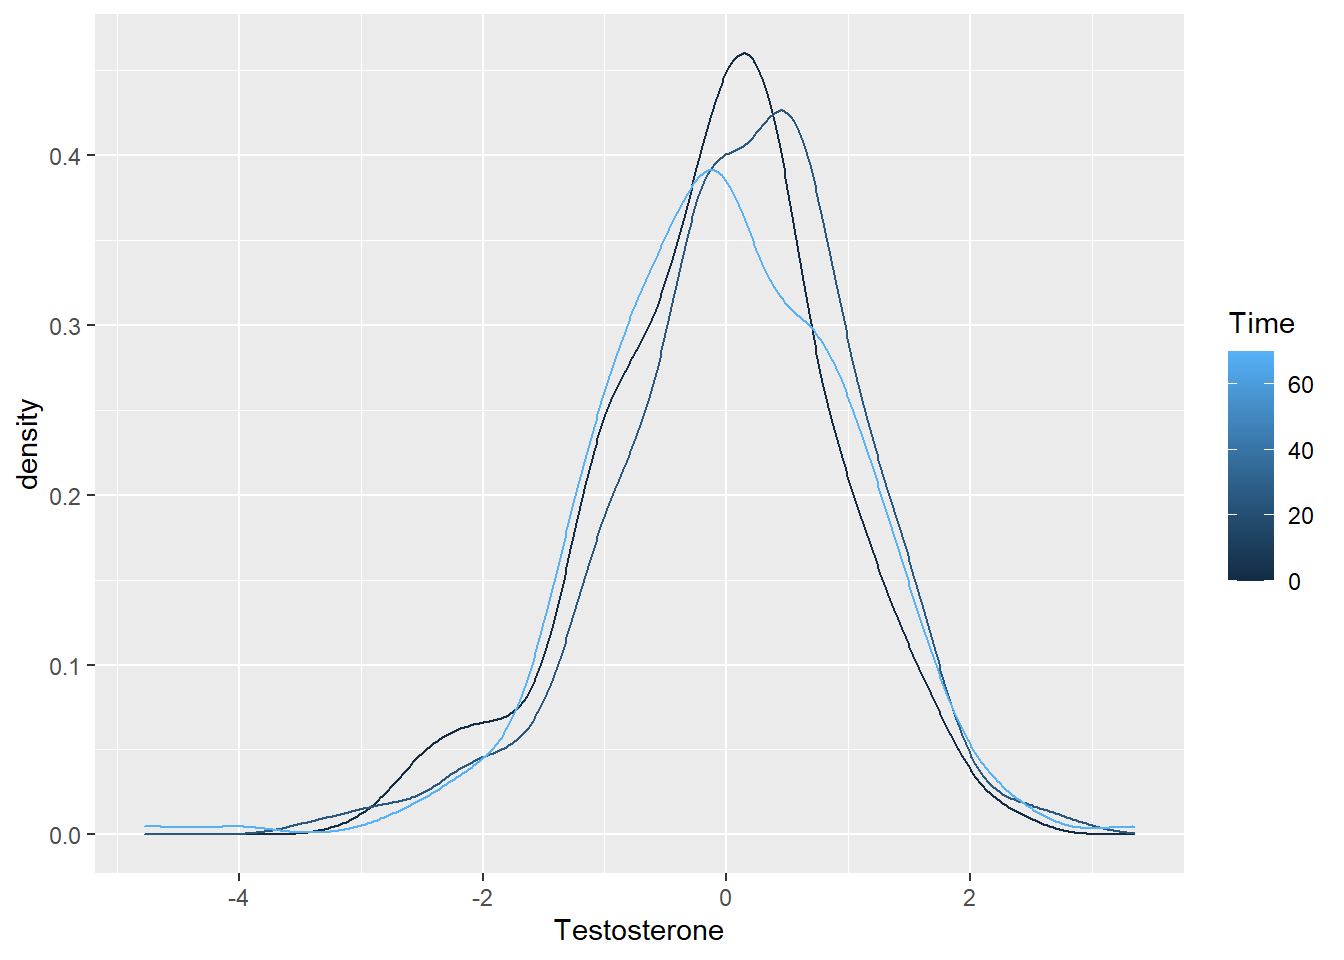
\includegraphics{01_Preprocessing_Modelling_files/figure-latex/wrap_res_TEST_2-1.pdf}

\begin{Shaded}
\begin{Highlighting}[]
\FunctionTok{ggplot}\NormalTok{(}\AttributeTok{data =}\NormalTok{ resall[[}\FunctionTok{paste0}\NormalTok{(depvar, }\StringTok{"\_longdat"}\NormalTok{)]], }
       \FunctionTok{aes}\NormalTok{(Time,DV, }\AttributeTok{col=}\NormalTok{group)) }\SpecialCharTok{+} 
  \FunctionTok{ylab}\NormalTok{(labeltag) }\SpecialCharTok{+} \FunctionTok{xlab}\NormalTok{(}\StringTok{"Time"}\NormalTok{)}\SpecialCharTok{+}
  \FunctionTok{geom\_smooth}\NormalTok{(}\AttributeTok{method =} \StringTok{\textquotesingle{}loess\textquotesingle{}}\NormalTok{) }\SpecialCharTok{+} \FunctionTok{geom\_point}\NormalTok{() }\SpecialCharTok{+}   \FunctionTok{facet\_wrap}\NormalTok{(}\SpecialCharTok{\textasciitilde{}}\NormalTok{gender)}
\end{Highlighting}
\end{Shaded}

\begin{verbatim}
## `geom_smooth()` using formula 'y ~ x'
\end{verbatim}

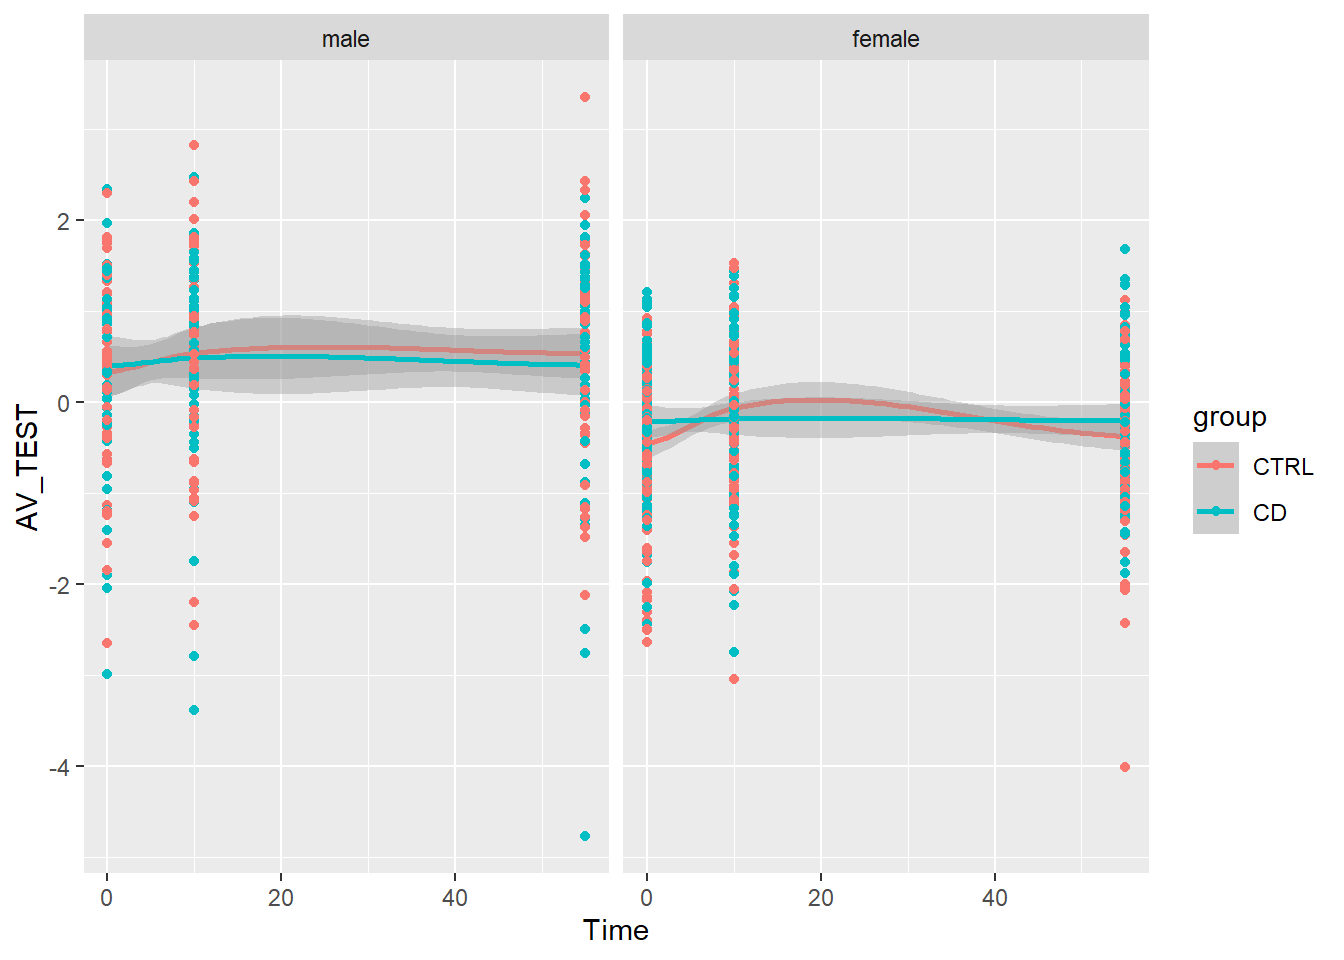
\includegraphics{01_Preprocessing_Modelling_files/figure-latex/wrap_res_TEST_2-2.pdf}

\hypertarget{sensitivity-analyses-2}{%
\paragraph{sensitivity analyses}\label{sensitivity-analyses-2}}

\begin{Shaded}
\begin{Highlighting}[]
\NormalTok{resall[[}\FunctionTok{paste0}\NormalTok{(depvar, }\StringTok{"\_coeff"}\NormalTok{)]] }\SpecialCharTok{\%\textgreater{}\%} \FunctionTok{tableplot}\NormalTok{()}
\end{Highlighting}
\end{Shaded}

\begin{table}
\centering
\begin{tabular}[t]{l|l|l|l|l}
\hline
  & Estimate & Std. Error & t value & pvalue\\
\hline
(Intercept) & 0.513 & 0.156 & 3.29 & 0.00099\\
\hline
age\_meancentered & 0.238 & 0.0546 & 4.35 & 1.34e-05\\
\hline
explstart\_meancentered\_min & -0.18 & 0.0482 & -3.74 & 0.000186\\
\hline
BMI\_imp\_meancentered & 0.17 & 0.0491 & 3.45 & 0.000552\\
\hline
any\_med\_cceptmed & -0.207 & 0.128 & -1.62 & 0.105\\
\hline
smoking\_yes\_nosmk & 0.162 & 0.132 & 1.23 & 0.219\\
\hline
genderfemale & -0.647 & 0.136 & -4.76 & 1.92e-06\\
\hline
groupCD & -0.0147 & 0.166 & -0.0887 & 0.929\\
\hline
poly(Time, 2)1 & 2.18 & 0.736 & 2.96 & 0.00308\\
\hline
poly(Time, 2)2 & -1.83 & 0.736 & -2.48 & 0.0131\\
\hline
genderfemale:groupCD & -0.0657 & 0.203 & -0.324 & 0.746\\
\hline
groupCD:poly(Time, 2)1 & -2.24 & 1.08 & -2.07 & 0.0383\\
\hline
groupCD:poly(Time, 2)2 & 0.671 & 1.08 & 0.619 & 0.536\\
\hline
genderfemale:poly(Time, 2)1 & -1.92 & 0.913 & -2.11 & 0.0351\\
\hline
genderfemale:poly(Time, 2)2 & -3.22 & 0.913 & -3.53 & 0.000411\\
\hline
genderfemale:groupCD:poly(Time, 2)1 & 2.07 & 1.35 & 1.53 & 0.127\\
\hline
genderfemale:groupCD:poly(Time, 2)2 & 3.96 & 1.35 & 2.93 & 0.00342\\
\hline
\end{tabular}
\end{table}

\begin{Shaded}
\begin{Highlighting}[]
\NormalTok{resall[[}\FunctionTok{paste0}\NormalTok{(depvar, }\StringTok{"\_coeff\_CDquant"}\NormalTok{)]] }\SpecialCharTok{\%\textgreater{}\%} \FunctionTok{tableplot}\NormalTok{()}
\end{Highlighting}
\end{Shaded}

\begin{table}
\centering
\begin{tabular}[t]{l|l|l|l|l}
\hline
  & Estimate & Std. Error & t value & pvalue\\
\hline
(Intercept) & 0.515 & 0.146 & 3.52 & 0.000424\\
\hline
age\_meancentered & 0.243 & 0.0536 & 4.53 & 6.04e-06\\
\hline
explstart\_meancentered\_min & -0.18 & 0.0481 & -3.74 & 0.000187\\
\hline
BMI\_imp\_meancentered & 0.166 & 0.0485 & 3.42 & 0.000634\\
\hline
any\_med\_cceptmed & -0.216 & 0.126 & -1.72 & 0.0855\\
\hline
smoking\_yes\_nosmk & 0.141 & 0.133 & 1.06 & 0.291\\
\hline
genderfemale & -0.674 & 0.106 & -6.36 & 1.99e-10\\
\hline
CDsymptomscurrent & 0.0359 & 0.0823 & 0.436 & 0.663\\
\hline
poly(Time, 2)1 & 1.15 & 0.545 & 2.11 & 0.0351\\
\hline
poly(Time, 2)2 & -1.53 & 0.545 & -2.81 & 0.00491\\
\hline
genderfemale:CDsymptomscurrent & -0.0716 & 0.0976 & -0.733 & 0.463\\
\hline
CDsymptomscurrent:poly(Time, 2)1 & -0.211 & 0.533 & -0.396 & 0.692\\
\hline
CDsymptomscurrent:poly(Time, 2)2 & 0.559 & 0.533 & 1.05 & 0.294\\
\hline
genderfemale:poly(Time, 2)1 & -0.974 & 0.681 & -1.43 & 0.152\\
\hline
genderfemale:poly(Time, 2)2 & -1.43 & 0.681 & -2.11 & 0.0351\\
\hline
genderfemale:CDsymptomscurrent:poly(Time, 2)1 & 0.079 & 0.674 & 0.117 & 0.907\\
\hline
genderfemale:CDsymptomscurrent:poly(Time, 2)2 & 1.47 & 0.674 & 2.19 & 0.0288\\
\hline
\end{tabular}
\end{table}

\begin{Shaded}
\begin{Highlighting}[]
\NormalTok{resall[[}\FunctionTok{paste0}\NormalTok{(depvar, }\StringTok{"\_coeff\_males"}\NormalTok{)]] }\SpecialCharTok{\%\textgreater{}\%} \FunctionTok{tableplot}\NormalTok{()}
\end{Highlighting}
\end{Shaded}

\begin{table}
\centering
\begin{tabular}[t]{l|l|l|l|l}
\hline
  & Estimate & Std. Error & t value & pvalue\\
\hline
(Intercept) & 0.419 & 0.18 & 2.33 & 0.0198\\
\hline
age\_meancentered & 0.478 & 0.0989 & 4.84 & 1.31e-06\\
\hline
explstart\_meancentered\_min & -0.311 & 0.0925 & -3.36 & 0.000779\\
\hline
BMI\_imp\_meancentered & 0.298 & 0.108 & 2.75 & 0.00596\\
\hline
any\_med\_cceptmed & 0.195 & 0.263 & 0.741 & 0.459\\
\hline
smoking\_yes\_nosmk & 0.246 & 0.224 & 1.1 & 0.273\\
\hline
groupCD & -0.118 & 0.181 & -0.65 & 0.516\\
\hline
poly(Time, 2)1 & 2.18 & 0.677 & 3.21 & 0.00131\\
\hline
poly(Time, 2)2 & -1.83 & 0.677 & -2.69 & 0.00705\\
\hline
groupCD:poly(Time, 2)1 & -2.24 & 0.997 & -2.25 & 0.0245\\
\hline
groupCD:poly(Time, 2)2 & 0.671 & 0.997 & 0.673 & 0.501\\
\hline
\end{tabular}
\end{table}

\begin{Shaded}
\begin{Highlighting}[]
\NormalTok{resall[[}\FunctionTok{paste0}\NormalTok{(depvar, }\StringTok{"\_coeff\_females"}\NormalTok{)]] }\SpecialCharTok{\%\textgreater{}\%} \FunctionTok{tableplot}\NormalTok{()}
\end{Highlighting}
\end{Shaded}

\begin{table}
\centering
\begin{tabular}[t]{l|l|l|l|l}
\hline
  & Estimate & Std. Error & t value & pvalue\\
\hline
(Intercept) & -0.17 & 0.126 & -1.35 & 0.177\\
\hline
age\_meancentered & 0.0873 & 0.0634 & 1.38 & 0.168\\
\hline
explstart\_meancentered\_min & -0.113 & 0.0532 & -2.12 & 0.0337\\
\hline
BMI\_imp\_meancentered & 0.123 & 0.0513 & 2.39 & 0.0168\\
\hline
any\_med\_cceptmed & -0.185 & 0.14 & -1.33 & 0.184\\
\hline
smoking\_yes\_nosmk & -0.0584 & 0.155 & -0.377 & 0.706\\
\hline
groupCD & 0.112 & 0.158 & 0.707 & 0.48\\
\hline
poly(Time, 2)1 & 0.254 & 0.562 & 0.452 & 0.651\\
\hline
poly(Time, 2)2 & -5.05 & 0.562 & -8.98 & 2.67e-19\\
\hline
groupCD:poly(Time, 2)1 & -0.175 & 0.847 & -0.207 & 0.836\\
\hline
groupCD:poly(Time, 2)2 & 4.63 & 0.847 & 5.47 & 4.41e-08\\
\hline
\end{tabular}
\end{table}

\begin{Shaded}
\begin{Highlighting}[]
\NormalTok{resall[[}\FunctionTok{paste0}\NormalTok{(depvar, }\StringTok{"\_coeff\_iq\_e\_total\_imp\_meancentered"}\NormalTok{)]] }\SpecialCharTok{\%\textgreater{}\%} \FunctionTok{tableplot}\NormalTok{()}
\end{Highlighting}
\end{Shaded}

\begin{table}
\centering
\begin{tabular}[t]{l|l|l|l|l}
\hline
  & Estimate & Std. Error & t value & pvalue\\
\hline
(Intercept) & 0.508 & 0.155 & 3.28 & 0.00103\\
\hline
iq\_e\_total\_imp\_meancentered & 0.0221 & 0.0511 & 0.432 & 0.666\\
\hline
age\_meancentered & 0.241 & 0.0551 & 4.37 & 1.26e-05\\
\hline
explstart\_meancentered\_min & -0.179 & 0.0483 & -3.7 & 0.000213\\
\hline
BMI\_imp\_meancentered & 0.171 & 0.0493 & 3.47 & 0.000523\\
\hline
any\_med\_cceptmed & -0.206 & 0.128 & -1.61 & 0.107\\
\hline
smoking\_yes\_nosmk & 0.167 & 0.132 & 1.26 & 0.208\\
\hline
genderfemale & -0.645 & 0.136 & -4.74 & 2.18e-06\\
\hline
groupCD & -0.00783 & 0.167 & -0.047 & 0.963\\
\hline
poly(Time, 2)1 & 2.18 & 0.736 & 2.96 & 0.00308\\
\hline
poly(Time, 2)2 & -1.83 & 0.736 & -2.48 & 0.0131\\
\hline
genderfemale:groupCD & -0.0654 & 0.203 & -0.322 & 0.747\\
\hline
groupCD:poly(Time, 2)1 & -2.24 & 1.08 & -2.07 & 0.0383\\
\hline
groupCD:poly(Time, 2)2 & 0.671 & 1.08 & 0.619 & 0.536\\
\hline
genderfemale:poly(Time, 2)1 & -1.92 & 0.913 & -2.11 & 0.0351\\
\hline
genderfemale:poly(Time, 2)2 & -3.22 & 0.913 & -3.53 & 0.000411\\
\hline
genderfemale:groupCD:poly(Time, 2)1 & 2.07 & 1.35 & 1.53 & 0.127\\
\hline
genderfemale:groupCD:poly(Time, 2)2 & 3.96 & 1.35 & 2.93 & 0.00342\\
\hline
\end{tabular}
\end{table}

\begin{Shaded}
\begin{Highlighting}[]
\NormalTok{resall[[}\FunctionTok{paste0}\NormalTok{(depvar, }\StringTok{"\_coeff\_EduParentsISCEDMean\_meancentered"}\NormalTok{)]] }\SpecialCharTok{\%\textgreater{}\%} \FunctionTok{tableplot}\NormalTok{()}
\end{Highlighting}
\end{Shaded}

\begin{table}
\centering
\begin{tabular}[t]{l|l|l|l|l}
\hline
  & Estimate & Std. Error & t value & pvalue\\
\hline
(Intercept) & 0.537 & 0.156 & 3.46 & 0.00055\\
\hline
EduParentsISCEDMean\_meancentered & 0.0745 & 0.0534 & 1.39 & 0.163\\
\hline
age\_meancentered & 0.251 & 0.057 & 4.4 & 1.06e-05\\
\hline
explstart\_meancentered\_min & -0.199 & 0.055 & -3.61 & 0.000301\\
\hline
BMI\_imp\_meancentered & 0.212 & 0.0595 & 3.57 & 0.000362\\
\hline
any\_med\_cceptmed & -0.277 & 0.135 & -2.06 & 0.0398\\
\hline
smoking\_yes\_nosmk & 0.133 & 0.139 & 0.954 & 0.34\\
\hline
genderfemale & -0.647 & 0.141 & -4.59 & 4.45e-06\\
\hline
groupCD & 0.0053 & 0.174 & 0.0305 & 0.976\\
\hline
poly(Time, 2)1 & 2.04 & 0.779 & 2.62 & 0.00868\\
\hline
poly(Time, 2)2 & -1.88 & 0.779 & -2.41 & 0.0158\\
\hline
genderfemale:groupCD & 0.092 & 0.217 & 0.423 & 0.672\\
\hline
groupCD:poly(Time, 2)1 & -2.9 & 1.16 & -2.51 & 0.0122\\
\hline
groupCD:poly(Time, 2)2 & 0.328 & 1.16 & 0.283 & 0.777\\
\hline
genderfemale:poly(Time, 2)1 & -1.8 & 0.971 & -1.86 & 0.063\\
\hline
genderfemale:poly(Time, 2)2 & -3.07 & 0.971 & -3.16 & 0.00156\\
\hline
genderfemale:groupCD:poly(Time, 2)1 & 2.78 & 1.46 & 1.9 & 0.0572\\
\hline
genderfemale:groupCD:poly(Time, 2)2 & 4.4 & 1.46 & 3.01 & 0.0026\\
\hline
\end{tabular}
\end{table}

\begin{Shaded}
\begin{Highlighting}[]
\NormalTok{resall[[}\FunctionTok{paste0}\NormalTok{(depvar, }\StringTok{"\_coeff\_pubcatimp\_meancentered"}\NormalTok{)]] }\SpecialCharTok{\%\textgreater{}\%} \FunctionTok{tableplot}\NormalTok{()}
\end{Highlighting}
\end{Shaded}

\begin{table}
\centering
\begin{tabular}[t]{l|l|l|l|l}
\hline
  & Estimate & Std. Error & t value & pvalue\\
\hline
(Intercept) & 0.631 & 0.165 & 3.83 & 0.000129\\
\hline
pubcatimp\_meancentered & 0.184 & 0.0727 & 2.54 & 0.0112\\
\hline
age\_meancentered & 0.138 & 0.067 & 2.05 & 0.0402\\
\hline
explstart\_meancentered\_min & -0.175 & 0.0478 & -3.67 & 0.000241\\
\hline
BMI\_imp\_meancentered & 0.151 & 0.0492 & 3.06 & 0.0022\\
\hline
any\_med\_cceptmed & -0.248 & 0.127 & -1.95 & 0.0512\\
\hline
smoking\_yes\_nosmk & 0.14 & 0.131 & 1.07 & 0.285\\
\hline
genderfemale & -0.826 & 0.152 & -5.43 & 5.5e-08\\
\hline
groupCD & -0.0258 & 0.164 & -0.157 & 0.875\\
\hline
poly(Time, 2)1 & 2.18 & 0.736 & 2.96 & 0.00308\\
\hline
poly(Time, 2)2 & -1.83 & 0.736 & -2.48 & 0.0131\\
\hline
genderfemale:groupCD & -0.0151 & 0.202 & -0.0747 & 0.94\\
\hline
groupCD:poly(Time, 2)1 & -2.24 & 1.08 & -2.07 & 0.0383\\
\hline
groupCD:poly(Time, 2)2 & 0.671 & 1.08 & 0.619 & 0.536\\
\hline
genderfemale:poly(Time, 2)1 & -1.92 & 0.913 & -2.11 & 0.0351\\
\hline
genderfemale:poly(Time, 2)2 & -3.22 & 0.913 & -3.53 & 0.000411\\
\hline
genderfemale:groupCD:poly(Time, 2)1 & 2.07 & 1.35 & 1.53 & 0.127\\
\hline
genderfemale:groupCD:poly(Time, 2)2 & 3.96 & 1.35 & 2.93 & 0.00342\\
\hline
\end{tabular}
\end{table}

\begin{Shaded}
\begin{Highlighting}[]
\NormalTok{resall[[}\FunctionTok{paste0}\NormalTok{(depvar, }\StringTok{"\_coeff\_ADHD\_life"}\NormalTok{)]] }\SpecialCharTok{\%\textgreater{}\%} \FunctionTok{tableplot}\NormalTok{()}
\end{Highlighting}
\end{Shaded}

\begin{table}
\centering
\begin{tabular}[t]{l|l|l|l|l}
\hline
  & Estimate & Std. Error & t value & pvalue\\
\hline
(Intercept) & 0.511 & 0.155 & 3.3 & 0.00098\\
\hline
ADHD\_lifeADHD & 0.0543 & 0.147 & 0.371 & 0.711\\
\hline
age\_meancentered & 0.238 & 0.0547 & 4.35 & 1.34e-05\\
\hline
explstart\_meancentered\_min & -0.18 & 0.0483 & -3.74 & 0.000186\\
\hline
BMI\_imp\_meancentered & 0.168 & 0.0493 & 3.42 & 0.000634\\
\hline
any\_med\_cceptmed & -0.206 & 0.128 & -1.61 & 0.108\\
\hline
smoking\_yes\_nosmk & 0.169 & 0.133 & 1.27 & 0.204\\
\hline
genderfemale & -0.647 & 0.136 & -4.75 & 2e-06\\
\hline
groupCD & -0.0483 & 0.189 & -0.256 & 0.798\\
\hline
poly(Time, 2)1 & 2.18 & 0.736 & 2.96 & 0.00308\\
\hline
poly(Time, 2)2 & -1.83 & 0.736 & -2.48 & 0.0131\\
\hline
genderfemale:groupCD & -0.0549 & 0.205 & -0.268 & 0.789\\
\hline
groupCD:poly(Time, 2)1 & -2.24 & 1.08 & -2.07 & 0.0383\\
\hline
groupCD:poly(Time, 2)2 & 0.671 & 1.08 & 0.619 & 0.536\\
\hline
genderfemale:poly(Time, 2)1 & -1.92 & 0.912 & -2.11 & 0.0351\\
\hline
genderfemale:poly(Time, 2)2 & -3.22 & 0.912 & -3.53 & 0.000411\\
\hline
genderfemale:groupCD:poly(Time, 2)1 & 2.07 & 1.35 & 1.53 & 0.127\\
\hline
genderfemale:groupCD:poly(Time, 2)2 & 3.96 & 1.35 & 2.93 & 0.00342\\
\hline
\end{tabular}
\end{table}

\begin{Shaded}
\begin{Highlighting}[]
\NormalTok{resall[[}\FunctionTok{paste0}\NormalTok{(depvar, }\StringTok{"\_coeff\_Depression\_lifetime"}\NormalTok{)]] }\SpecialCharTok{\%\textgreater{}\%} \FunctionTok{tableplot}\NormalTok{()}
\end{Highlighting}
\end{Shaded}

\begin{table}
\centering
\begin{tabular}[t]{l|l|l|l|l}
\hline
  & Estimate & Std. Error & t value & pvalue\\
\hline
(Intercept) & 0.514 & 0.155 & 3.33 & 0.000874\\
\hline
Depression\_lifetimeDepression & 0.0762 & 0.147 & 0.519 & 0.604\\
\hline
age\_meancentered & 0.24 & 0.0548 & 4.37 & 1.22e-05\\
\hline
explstart\_meancentered\_min & -0.179 & 0.0483 & -3.69 & 0.000221\\
\hline
BMI\_imp\_meancentered & 0.172 & 0.0494 & 3.48 & 0.000496\\
\hline
any\_med\_cceptmed & -0.217 & 0.129 & -1.68 & 0.0933\\
\hline
smoking\_yes\_nosmk & 0.155 & 0.133 & 1.17 & 0.244\\
\hline
genderfemale & -0.65 & 0.136 & -4.77 & 1.82e-06\\
\hline
groupCD & -0.0243 & 0.167 & -0.146 & 0.884\\
\hline
poly(Time, 2)1 & 2.18 & 0.736 & 2.96 & 0.00308\\
\hline
poly(Time, 2)2 & -1.83 & 0.736 & -2.48 & 0.0131\\
\hline
genderfemale:groupCD & -0.0779 & 0.205 & -0.381 & 0.703\\
\hline
groupCD:poly(Time, 2)1 & -2.24 & 1.08 & -2.07 & 0.0383\\
\hline
groupCD:poly(Time, 2)2 & 0.671 & 1.08 & 0.619 & 0.536\\
\hline
genderfemale:poly(Time, 2)1 & -1.92 & 0.913 & -2.11 & 0.0351\\
\hline
genderfemale:poly(Time, 2)2 & -3.22 & 0.913 & -3.53 & 0.000411\\
\hline
genderfemale:groupCD:poly(Time, 2)1 & 2.07 & 1.35 & 1.53 & 0.127\\
\hline
genderfemale:groupCD:poly(Time, 2)2 & 3.96 & 1.35 & 2.93 & 0.00342\\
\hline
\end{tabular}
\end{table}

\begin{Shaded}
\begin{Highlighting}[]
\NormalTok{resall[[}\FunctionTok{paste0}\NormalTok{(depvar, }\StringTok{"\_coeff\_PTSD\_lifetime"}\NormalTok{)]] }\SpecialCharTok{\%\textgreater{}\%} \FunctionTok{tableplot}\NormalTok{()}
\end{Highlighting}
\end{Shaded}

\begin{table}
\centering
\begin{tabular}[t]{l|l|l|l|l}
\hline
  & Estimate & Std. Error & t value & pvalue\\
\hline
(Intercept) & 0.514 & 0.156 & 3.28 & 0.00103\\
\hline
PTSD\_lifetimePTSD & 0.0475 & 0.201 & 0.236 & 0.813\\
\hline
age\_meancentered & 0.238 & 0.0547 & 4.34 & 1.42e-05\\
\hline
explstart\_meancentered\_min & -0.18 & 0.0483 & -3.74 & 0.000187\\
\hline
BMI\_imp\_meancentered & 0.17 & 0.0492 & 3.45 & 0.000565\\
\hline
any\_med\_cceptmed & -0.209 & 0.128 & -1.63 & 0.103\\
\hline
smoking\_yes\_nosmk & 0.16 & 0.132 & 1.21 & 0.226\\
\hline
genderfemale & -0.647 & 0.136 & -4.75 & 2.04e-06\\
\hline
groupCD & -0.0172 & 0.166 & -0.104 & 0.917\\
\hline
poly(Time, 2)1 & 2.18 & 0.736 & 2.96 & 0.00308\\
\hline
poly(Time, 2)2 & -1.83 & 0.736 & -2.48 & 0.0131\\
\hline
genderfemale:groupCD & -0.0673 & 0.203 & -0.331 & 0.741\\
\hline
groupCD:poly(Time, 2)1 & -2.24 & 1.08 & -2.07 & 0.0383\\
\hline
groupCD:poly(Time, 2)2 & 0.671 & 1.08 & 0.619 & 0.536\\
\hline
genderfemale:poly(Time, 2)1 & -1.92 & 0.912 & -2.11 & 0.0351\\
\hline
genderfemale:poly(Time, 2)2 & -3.22 & 0.912 & -3.53 & 0.000411\\
\hline
genderfemale:groupCD:poly(Time, 2)1 & 2.07 & 1.35 & 1.53 & 0.127\\
\hline
genderfemale:groupCD:poly(Time, 2)2 & 3.96 & 1.35 & 2.93 & 0.00342\\
\hline
\end{tabular}
\end{table}

\begin{Shaded}
\begin{Highlighting}[]
\NormalTok{resall[[}\FunctionTok{paste0}\NormalTok{(depvar, }\StringTok{"\_coeff\_SUD\_life"}\NormalTok{)]] }\SpecialCharTok{\%\textgreater{}\%} \FunctionTok{tableplot}\NormalTok{()}
\end{Highlighting}
\end{Shaded}

\begin{table}
\centering
\begin{tabular}[t]{l|l|l|l|l}
\hline
  & Estimate & Std. Error & t value & pvalue\\
\hline
(Intercept) & 0.513 & 0.157 & 3.27 & 0.00106\\
\hline
SUD\_lifeSUD & 0.163 & 0.177 & 0.923 & 0.356\\
\hline
age\_meancentered & 0.231 & 0.0551 & 4.19 & 2.76e-05\\
\hline
explstart\_meancentered\_min & -0.182 & 0.0483 & -3.78 & 0.000159\\
\hline
BMI\_imp\_meancentered & 0.175 & 0.0494 & 3.54 & 0.000404\\
\hline
any\_med\_cceptmed & -0.217 & 0.128 & -1.69 & 0.0903\\
\hline
smoking\_yes\_nosmk & 0.125 & 0.138 & 0.905 & 0.365\\
\hline
genderfemale & -0.643 & 0.136 & -4.72 & 2.33e-06\\
\hline
groupCD & -0.0443 & 0.169 & -0.263 & 0.793\\
\hline
poly(Time, 2)1 & 2.18 & 0.736 & 2.96 & 0.00308\\
\hline
poly(Time, 2)2 & -1.83 & 0.736 & -2.48 & 0.0131\\
\hline
genderfemale:groupCD & -0.0484 & 0.204 & -0.237 & 0.812\\
\hline
groupCD:poly(Time, 2)1 & -2.24 & 1.08 & -2.07 & 0.0383\\
\hline
groupCD:poly(Time, 2)2 & 0.671 & 1.08 & 0.619 & 0.536\\
\hline
genderfemale:poly(Time, 2)1 & -1.92 & 0.913 & -2.11 & 0.0351\\
\hline
genderfemale:poly(Time, 2)2 & -3.22 & 0.913 & -3.53 & 0.000411\\
\hline
genderfemale:groupCD:poly(Time, 2)1 & 2.07 & 1.35 & 1.53 & 0.127\\
\hline
genderfemale:groupCD:poly(Time, 2)2 & 3.96 & 1.35 & 2.93 & 0.00342\\
\hline
\end{tabular}
\end{table}

\begin{Shaded}
\begin{Highlighting}[]
\NormalTok{resall[[}\FunctionTok{paste0}\NormalTok{(depvar, }\StringTok{"\_coeff\_Anxiety\_lifetime"}\NormalTok{)]] }\SpecialCharTok{\%\textgreater{}\%} \FunctionTok{tableplot}\NormalTok{()}
\end{Highlighting}
\end{Shaded}

\begin{table}
\centering
\begin{tabular}[t]{l|l|l|l|l}
\hline
  & Estimate & Std. Error & t value & pvalue\\
\hline
(Intercept) & 0.502 & 0.149 & 3.36 & 0.000772\\
\hline
Anxiety\_lifetimeAnxiety & 0.216 & 0.154 & 1.4 & 0.162\\
\hline
age\_meancentered & 0.241 & 0.0545 & 4.42 & 9.94e-06\\
\hline
explstart\_meancentered\_min & -0.178 & 0.0481 & -3.71 & 0.000211\\
\hline
BMI\_imp\_meancentered & 0.175 & 0.0492 & 3.55 & 0.000381\\
\hline
any\_med\_cceptmed & -0.239 & 0.129 & -1.85 & 0.0646\\
\hline
smoking\_yes\_nosmk & 0.173 & 0.132 & 1.31 & 0.19\\
\hline
genderfemale & -0.645 & 0.136 & -4.75 & 2e-06\\
\hline
groupCD & -0.081 & 0.172 & -0.471 & 0.638\\
\hline
poly(Time, 2)1 & 2.18 & 0.736 & 2.96 & 0.00308\\
\hline
poly(Time, 2)2 & -1.83 & 0.736 & -2.48 & 0.0131\\
\hline
genderfemale:groupCD & -0.0294 & 0.204 & -0.144 & 0.885\\
\hline
groupCD:poly(Time, 2)1 & -2.24 & 1.08 & -2.07 & 0.0383\\
\hline
groupCD:poly(Time, 2)2 & 0.671 & 1.08 & 0.619 & 0.536\\
\hline
genderfemale:poly(Time, 2)1 & -1.92 & 0.913 & -2.11 & 0.0351\\
\hline
genderfemale:poly(Time, 2)2 & -3.22 & 0.913 & -3.53 & 0.000411\\
\hline
genderfemale:groupCD:poly(Time, 2)1 & 2.07 & 1.35 & 1.53 & 0.127\\
\hline
genderfemale:groupCD:poly(Time, 2)2 & 3.96 & 1.35 & 2.93 & 0.00342\\
\hline
\end{tabular}
\end{table}

\hypertarget{testcort-ratio}{%
\subsubsection{TEST/CORT ratio}\label{testcort-ratio}}

full models:
DV\textasciitilde1+age\_meancentered+explstart\_meancentered\_min+BMI\_imp\_meancentered+any\_med\_ccept+smoking\_yes\_no+gender+group+poly(Time,
2)+gender\emph{group+poly(Time, 2)}group+gender\emph{poly(Time,
2)}group+(1\textbar twuid)+(1\textbar centre)

h0 model: DV\textasciitilde1+(1\textbar twuid)+(1\textbar centre):

overall model p-value: 1.16e-22

\begin{Shaded}
\begin{Highlighting}[]
\NormalTok{depvar }\OtherTok{=} \StringTok{"AV\_TESTCORT"}
\NormalTok{labeltag }\OtherTok{=} \StringTok{"Testosterone/Cortisol ratio"}

\FunctionTok{ggplot}\NormalTok{(}\AttributeTok{data =}\NormalTok{ resall[[}\FunctionTok{paste0}\NormalTok{(depvar, }\StringTok{"\_longdat"}\NormalTok{)]], }
       \FunctionTok{aes}\NormalTok{(DV, }\AttributeTok{group=}\NormalTok{Time, }\AttributeTok{col=}\NormalTok{Time)) }\SpecialCharTok{+} 
  \FunctionTok{ylab}\NormalTok{(}\StringTok{"density"}\NormalTok{) }\SpecialCharTok{+} \FunctionTok{xlab}\NormalTok{(labeltag)}\SpecialCharTok{+}
  \FunctionTok{geom\_density}\NormalTok{()}
\end{Highlighting}
\end{Shaded}

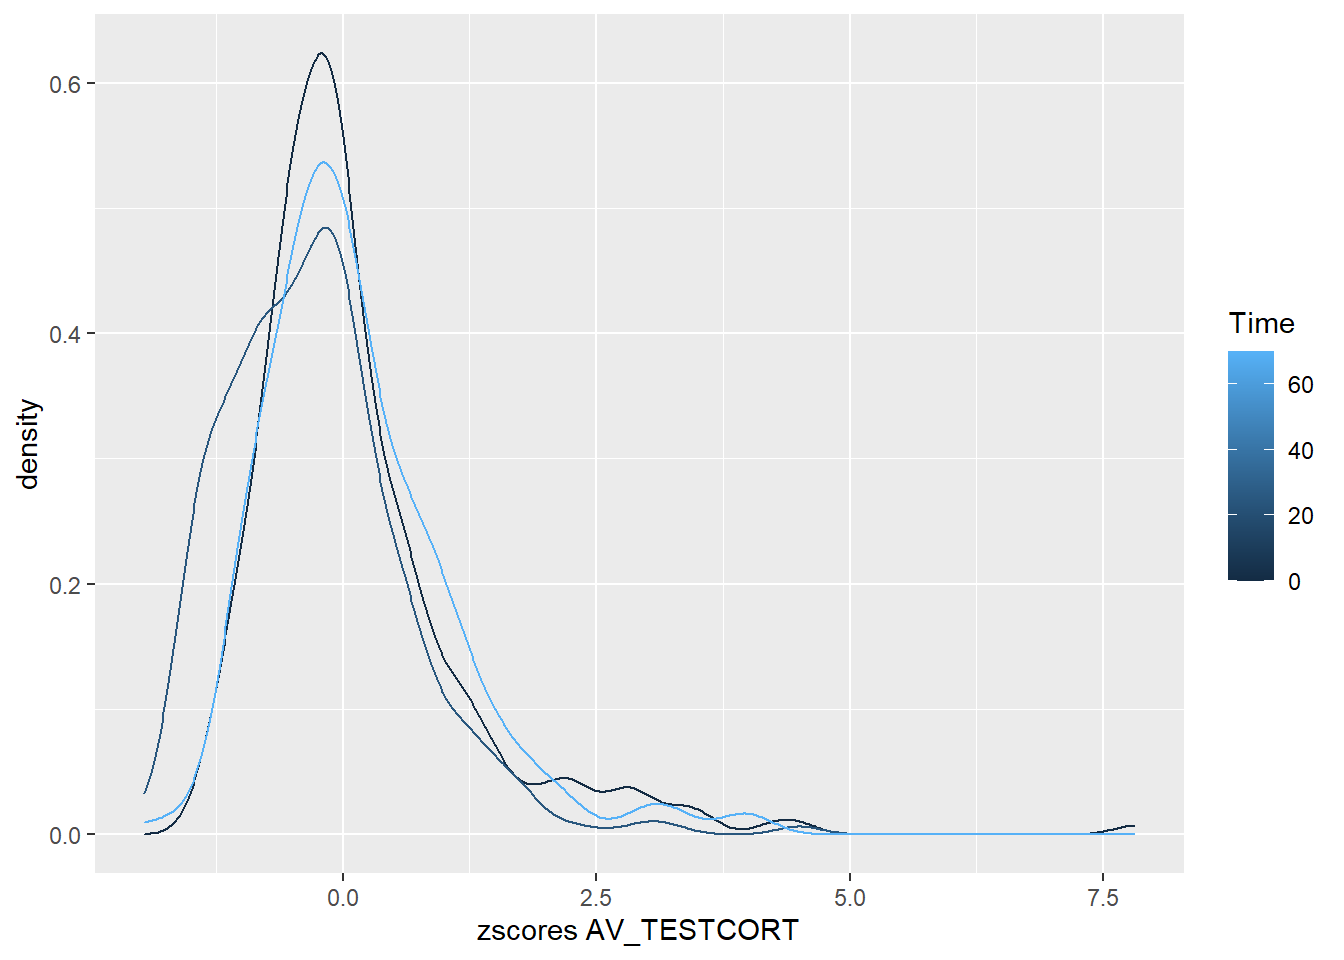
\includegraphics{01_Preprocessing_Modelling_files/figure-latex/wrap_res_testcort_2-1.pdf}

\begin{Shaded}
\begin{Highlighting}[]
\FunctionTok{ggplot}\NormalTok{(}\AttributeTok{data =}\NormalTok{ resall[[}\FunctionTok{paste0}\NormalTok{(depvar, }\StringTok{"\_longdat"}\NormalTok{)]], }
       \FunctionTok{aes}\NormalTok{(Time,DV, }\AttributeTok{col=}\NormalTok{group)) }\SpecialCharTok{+} 
  \FunctionTok{ylab}\NormalTok{(labeltag) }\SpecialCharTok{+} \FunctionTok{xlab}\NormalTok{(}\StringTok{"Time"}\NormalTok{)}\SpecialCharTok{+}
  \FunctionTok{geom\_smooth}\NormalTok{(}\AttributeTok{method =} \StringTok{\textquotesingle{}loess\textquotesingle{}}\NormalTok{) }\SpecialCharTok{+} \FunctionTok{geom\_point}\NormalTok{() }\SpecialCharTok{+}   \FunctionTok{facet\_wrap}\NormalTok{(}\SpecialCharTok{\textasciitilde{}}\NormalTok{gender)}
\end{Highlighting}
\end{Shaded}

\begin{verbatim}
## `geom_smooth()` using formula 'y ~ x'
\end{verbatim}

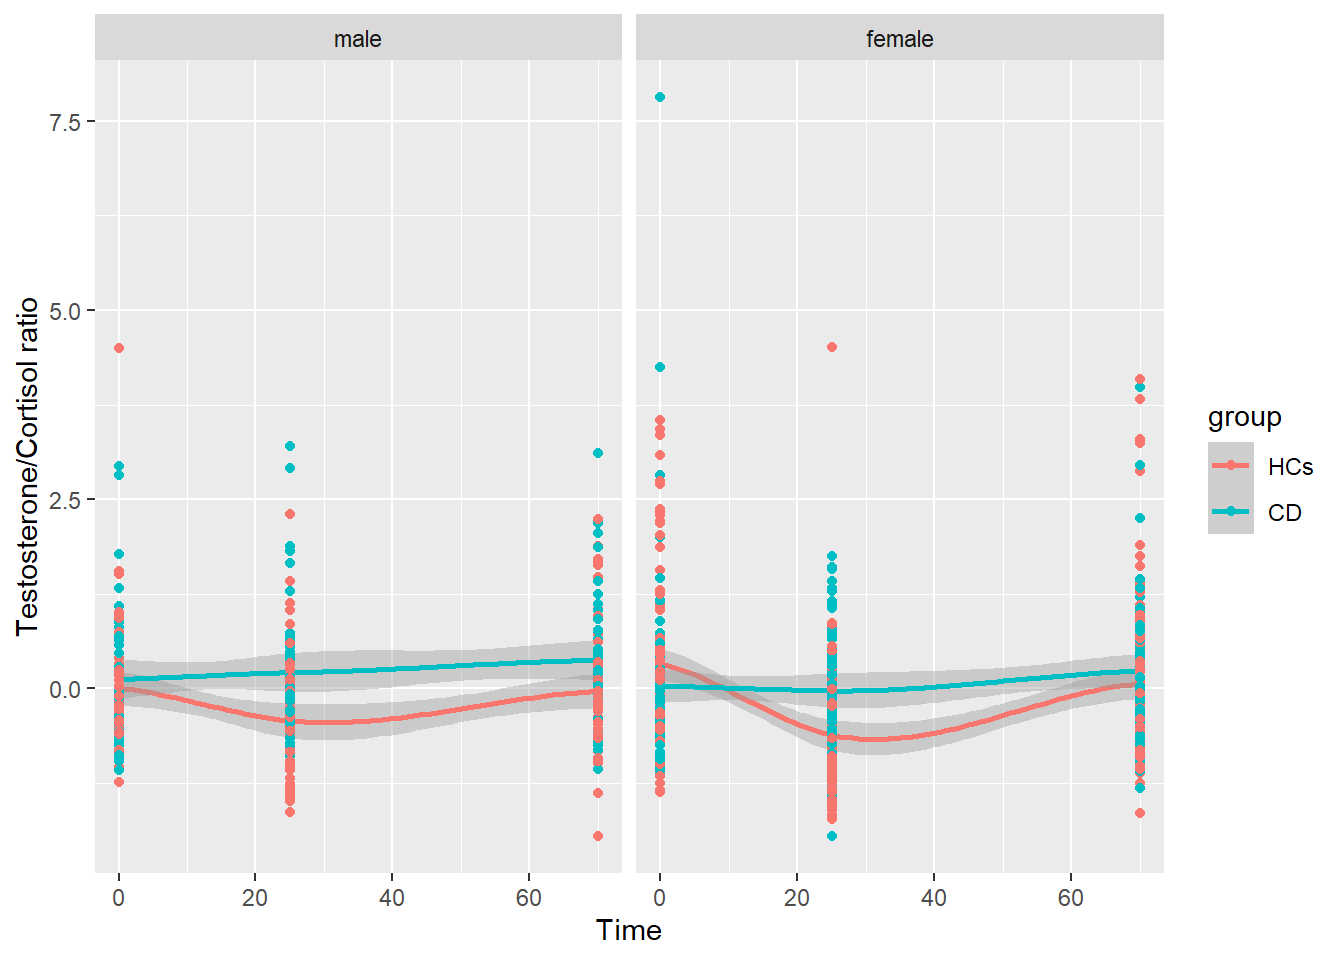
\includegraphics{01_Preprocessing_Modelling_files/figure-latex/wrap_res_testcort_2-2.pdf}

\hypertarget{sensitivity-analyses-3}{%
\paragraph{sensitivity analyses}\label{sensitivity-analyses-3}}

\begin{Shaded}
\begin{Highlighting}[]
\NormalTok{resall[[}\FunctionTok{paste0}\NormalTok{(depvar, }\StringTok{"\_coeff"}\NormalTok{)]] }\SpecialCharTok{\%\textgreater{}\%} \FunctionTok{tableplot}\NormalTok{()}
\end{Highlighting}
\end{Shaded}

\begin{table}
\centering
\begin{tabular}[t]{l|l|l|l|l}
\hline
  & Estimate & Std. Error & t value & pvalue\\
\hline
(Intercept) & -0.0623 & 0.114 & -0.548 & 0.584\\
\hline
age\_meancentered & -0.185 & 0.0515 & -3.59 & 0.000333\\
\hline
explstart\_meancentered\_min & 0.16 & 0.0464 & 3.45 & 0.000562\\
\hline
BMI\_imp\_meancentered & -0.0288 & 0.047 & -0.612 & 0.54\\
\hline
any\_med\_cceptmed & -0.0695 & 0.122 & -0.57 & 0.569\\
\hline
smoking\_yes\_nosmk & 0.0939 & 0.125 & 0.751 & 0.453\\
\hline
genderfemale & 0.0231 & 0.128 & 0.18 & 0.857\\
\hline
groupCD & 0.339 & 0.159 & 2.13 & 0.0328\\
\hline
poly(Time, 2)1 & 0.415 & 1.68 & 0.248 & 0.804\\
\hline
poly(Time, 2)2 & 5.85 & 1.67 & 3.51 & 0.000442\\
\hline
genderfemale:groupCD & -0.154 & 0.193 & -0.797 & 0.425\\
\hline
groupCD:poly(Time, 2)1 & 3.11 & 2.49 & 1.25 & 0.211\\
\hline
groupCD:poly(Time, 2)2 & -5.43 & 2.45 & -2.21 & 0.0268\\
\hline
genderfemale:poly(Time, 2)1 & -1.52 & 2.1 & -0.725 & 0.468\\
\hline
genderfemale:poly(Time, 2)2 & 6.09 & 2.08 & 2.94 & 0.00333\\
\hline
genderfemale:groupCD:poly(Time, 2)1 & 1.04 & 3.13 & 0.334 & 0.739\\
\hline
genderfemale:groupCD:poly(Time, 2)2 & -4.5 & 3.09 & -1.46 & 0.145\\
\hline
\end{tabular}
\end{table}

\begin{Shaded}
\begin{Highlighting}[]
\NormalTok{resall[[}\FunctionTok{paste0}\NormalTok{(depvar, }\StringTok{"\_coeff\_CDquant"}\NormalTok{)]] }\SpecialCharTok{\%\textgreater{}\%} \FunctionTok{tableplot}\NormalTok{()}
\end{Highlighting}
\end{Shaded}

\begin{table}
\centering
\begin{tabular}[t]{l|l|l|l|l}
\hline
  & Estimate & Std. Error & t value & pvalue\\
\hline
(Intercept) & 0.0871 & 0.0943 & 0.923 & 0.356\\
\hline
age\_meancentered & -0.192 & 0.0502 & -3.82 & 0.000134\\
\hline
explstart\_meancentered\_min & 0.158 & 0.046 & 3.44 & 0.000578\\
\hline
BMI\_imp\_meancentered & -0.0254 & 0.0463 & -0.549 & 0.583\\
\hline
any\_med\_cceptmed & -0.0977 & 0.119 & -0.819 & 0.413\\
\hline
smoking\_yes\_nosmk & 0.0736 & 0.126 & 0.584 & 0.559\\
\hline
genderfemale & -0.0357 & 0.0982 & -0.363 & 0.717\\
\hline
CDsymptomscurrent & 0.0892 & 0.0782 & 1.14 & 0.254\\
\hline
poly(Time, 2)1 & 1.74 & 1.26 & 1.38 & 0.168\\
\hline
poly(Time, 2)2 & 3.44 & 1.24 & 2.76 & 0.00575\\
\hline
genderfemale:CDsymptomscurrent & 0.0679 & 0.0926 & 0.734 & 0.463\\
\hline
CDsymptomscurrent:poly(Time, 2)1 & 1.8 & 1.2 & 1.49 & 0.135\\
\hline
CDsymptomscurrent:poly(Time, 2)2 & -2.27 & 1.2 & -1.89 & 0.0583\\
\hline
genderfemale:poly(Time, 2)1 & -0.984 & 1.58 & -0.622 & 0.534\\
\hline
genderfemale:poly(Time, 2)2 & 4.11 & 1.56 & 2.63 & 0.00863\\
\hline
genderfemale:CDsymptomscurrent:poly(Time, 2)1 & -0.99 & 1.54 & -0.642 & 0.521\\
\hline
genderfemale:CDsymptomscurrent:poly(Time, 2)2 & -1.45 & 1.53 & -0.948 & 0.343\\
\hline
\end{tabular}
\end{table}

\begin{Shaded}
\begin{Highlighting}[]
\NormalTok{resall[[}\FunctionTok{paste0}\NormalTok{(depvar, }\StringTok{"\_coeff\_males"}\NormalTok{)]] }\SpecialCharTok{\%\textgreater{}\%} \FunctionTok{tableplot}\NormalTok{()}
\end{Highlighting}
\end{Shaded}

\begin{table}
\centering
\begin{tabular}[t]{l|l|l|l|l}
\hline
  & Estimate & Std. Error & t value & pvalue\\
\hline
(Intercept) & -0.0936 & 0.102 & -0.914 & 0.361\\
\hline
age\_meancentered & -0.0833 & 0.0866 & -0.961 & 0.336\\
\hline
explstart\_meancentered\_min & 0.175 & 0.0792 & 2.21 & 0.0271\\
\hline
BMI\_imp\_meancentered & -0.0978 & 0.0964 & -1.01 & 0.31\\
\hline
any\_med\_cceptmed & -0.207 & 0.238 & -0.868 & 0.385\\
\hline
smoking\_yes\_nosmk & 0.00756 & 0.197 & 0.0384 & 0.969\\
\hline
groupCD & 0.418 & 0.163 & 2.56 & 0.0104\\
\hline
poly(Time, 2)1 & 0.409 & 1.41 & 0.29 & 0.772\\
\hline
poly(Time, 2)2 & 5.84 & 1.41 & 4.16 & 3.21e-05\\
\hline
groupCD:poly(Time, 2)1 & 3.13 & 2.1 & 1.49 & 0.136\\
\hline
groupCD:poly(Time, 2)2 & -5.4 & 2.07 & -2.61 & 0.0091\\
\hline
\end{tabular}
\end{table}

\begin{Shaded}
\begin{Highlighting}[]
\NormalTok{resall[[}\FunctionTok{paste0}\NormalTok{(depvar, }\StringTok{"\_coeff\_females"}\NormalTok{)]] }\SpecialCharTok{\%\textgreater{}\%} \FunctionTok{tableplot}\NormalTok{()}
\end{Highlighting}
\end{Shaded}

\begin{table}
\centering
\begin{tabular}[t]{l|l|l|l|l}
\hline
  & Estimate & Std. Error & t value & pvalue\\
\hline
(Intercept) & -0.047 & 0.0985 & -0.477 & 0.633\\
\hline
age\_meancentered & -0.248 & 0.0677 & -3.66 & 0.00025\\
\hline
explstart\_meancentered\_min & 0.16 & 0.0575 & 2.78 & 0.0054\\
\hline
BMI\_imp\_meancentered & -0.0123 & 0.0548 & -0.225 & 0.822\\
\hline
any\_med\_cceptmed & 0.0282 & 0.149 & 0.19 & 0.849\\
\hline
smoking\_yes\_nosmk & 0.133 & 0.165 & 0.804 & 0.421\\
\hline
groupCD & 0.116 & 0.168 & 0.687 & 0.492\\
\hline
poly(Time, 2)1 & -1.14 & 1.36 & -0.835 & 0.404\\
\hline
poly(Time, 2)2 & 11.9 & 1.34 & 8.93 & 4.16e-19\\
\hline
groupCD:poly(Time, 2)1 & 4.17 & 2.05 & 2.04 & 0.0417\\
\hline
groupCD:poly(Time, 2)2 & -9.93 & 2.03 & -4.9 & 9.71e-07\\
\hline
\end{tabular}
\end{table}

\begin{Shaded}
\begin{Highlighting}[]
\NormalTok{resall[[}\FunctionTok{paste0}\NormalTok{(depvar, }\StringTok{"\_coeff\_iq\_e\_total\_imp\_meancentered"}\NormalTok{)]] }\SpecialCharTok{\%\textgreater{}\%} \FunctionTok{tableplot}\NormalTok{()}
\end{Highlighting}
\end{Shaded}

\begin{table}
\centering
\begin{tabular}[t]{l|l|l|l|l}
\hline
  & Estimate & Std. Error & t value & pvalue\\
\hline
(Intercept) & -0.0705 & 0.116 & -0.61 & 0.542\\
\hline
iq\_e\_total\_imp\_meancentered & 0.0445 & 0.0481 & 0.925 & 0.355\\
\hline
age\_meancentered & -0.18 & 0.0521 & -3.45 & 0.000559\\
\hline
explstart\_meancentered\_min & 0.161 & 0.0464 & 3.47 & 0.000519\\
\hline
BMI\_imp\_meancentered & -0.0258 & 0.0471 & -0.547 & 0.585\\
\hline
any\_med\_cceptmed & -0.0661 & 0.122 & -0.541 & 0.589\\
\hline
smoking\_yes\_nosmk & 0.101 & 0.126 & 0.806 & 0.42\\
\hline
genderfemale & 0.0275 & 0.129 & 0.213 & 0.831\\
\hline
groupCD & 0.354 & 0.16 & 2.22 & 0.0266\\
\hline
poly(Time, 2)1 & 0.413 & 1.68 & 0.246 & 0.805\\
\hline
poly(Time, 2)2 & 5.86 & 1.67 & 3.52 & 0.000431\\
\hline
genderfemale:groupCD & -0.154 & 0.194 & -0.794 & 0.427\\
\hline
groupCD:poly(Time, 2)1 & 3.1 & 2.49 & 1.24 & 0.213\\
\hline
groupCD:poly(Time, 2)2 & -5.43 & 2.45 & -2.22 & 0.0267\\
\hline
genderfemale:poly(Time, 2)1 & -1.5 & 2.09 & -0.718 & 0.473\\
\hline
genderfemale:poly(Time, 2)2 & 6.08 & 2.07 & 2.93 & 0.00336\\
\hline
genderfemale:groupCD:poly(Time, 2)1 & 1.05 & 3.13 & 0.337 & 0.736\\
\hline
genderfemale:groupCD:poly(Time, 2)2 & -4.5 & 3.09 & -1.46 & 0.145\\
\hline
\end{tabular}
\end{table}

\begin{Shaded}
\begin{Highlighting}[]
\NormalTok{resall[[}\FunctionTok{paste0}\NormalTok{(depvar, }\StringTok{"\_coeff\_EduParentsISCEDMean\_meancentered"}\NormalTok{)]] }\SpecialCharTok{\%\textgreater{}\%} \FunctionTok{tableplot}\NormalTok{()}
\end{Highlighting}
\end{Shaded}

\begin{table}
\centering
\begin{tabular}[t]{l|l|l|l|l}
\hline
  & Estimate & Std. Error & t value & pvalue\\
\hline
(Intercept) & -0.0802 & 0.122 & -0.659 & 0.51\\
\hline
EduParentsISCEDMean\_meancentered & 0.052 & 0.0529 & 0.983 & 0.326\\
\hline
age\_meancentered & -0.184 & 0.0562 & -3.28 & 0.00105\\
\hline
explstart\_meancentered\_min & 0.186 & 0.0552 & 3.37 & 0.000755\\
\hline
BMI\_imp\_meancentered & -0.0508 & 0.0591 & -0.86 & 0.39\\
\hline
any\_med\_cceptmed & -0.161 & 0.134 & -1.2 & 0.231\\
\hline
smoking\_yes\_nosmk & 0.16 & 0.137 & 1.17 & 0.241\\
\hline
genderfemale & 0.00575 & 0.138 & 0.0416 & 0.967\\
\hline
groupCD & 0.368 & 0.172 & 2.13 & 0.0328\\
\hline
poly(Time, 2)1 & 0.491 & 1.81 & 0.27 & 0.787\\
\hline
poly(Time, 2)2 & 5.39 & 1.8 & 2.99 & 0.00279\\
\hline
genderfemale:groupCD & -0.0541 & 0.215 & -0.252 & 0.801\\
\hline
groupCD:poly(Time, 2)1 & 3.46 & 2.73 & 1.27 & 0.206\\
\hline
groupCD:poly(Time, 2)2 & -3.86 & 2.69 & -1.44 & 0.151\\
\hline
genderfemale:poly(Time, 2)1 & -0.938 & 2.28 & -0.412 & 0.681\\
\hline
genderfemale:poly(Time, 2)2 & 6.12 & 2.26 & 2.71 & 0.00672\\
\hline
genderfemale:groupCD:poly(Time, 2)1 & -0.108 & 3.46 & -0.0311 & 0.975\\
\hline
genderfemale:groupCD:poly(Time, 2)2 & -5.08 & 3.41 & -1.49 & 0.136\\
\hline
\end{tabular}
\end{table}

\begin{Shaded}
\begin{Highlighting}[]
\NormalTok{resall[[}\FunctionTok{paste0}\NormalTok{(depvar, }\StringTok{"\_coeff\_pubcatimp\_meancentered"}\NormalTok{)]] }\SpecialCharTok{\%\textgreater{}\%} \FunctionTok{tableplot}\NormalTok{()}
\end{Highlighting}
\end{Shaded}

\begin{table}
\centering
\begin{tabular}[t]{l|l|l|l|l}
\hline
  & Estimate & Std. Error & t value & pvalue\\
\hline
(Intercept) & -0.152 & 0.125 & -1.22 & 0.222\\
\hline
pubcatimp\_meancentered & -0.155 & 0.0693 & -2.24 & 0.0251\\
\hline
age\_meancentered & -0.0997 & 0.0643 & -1.55 & 0.121\\
\hline
explstart\_meancentered\_min & 0.155 & 0.0462 & 3.35 & 0.000798\\
\hline
BMI\_imp\_meancentered & -0.0121 & 0.0472 & -0.256 & 0.798\\
\hline
any\_med\_cceptmed & -0.0319 & 0.122 & -0.261 & 0.794\\
\hline
smoking\_yes\_nosmk & 0.104 & 0.125 & 0.831 & 0.406\\
\hline
genderfemale & 0.171 & 0.145 & 1.18 & 0.237\\
\hline
groupCD & 0.352 & 0.158 & 2.23 & 0.0256\\
\hline
poly(Time, 2)1 & 0.393 & 1.68 & 0.235 & 0.815\\
\hline
poly(Time, 2)2 & 5.87 & 1.67 & 3.52 & 0.000425\\
\hline
genderfemale:groupCD & -0.2 & 0.193 & -1.04 & 0.3\\
\hline
groupCD:poly(Time, 2)1 & 3.09 & 2.49 & 1.24 & 0.214\\
\hline
groupCD:poly(Time, 2)2 & -5.49 & 2.45 & -2.24 & 0.0252\\
\hline
genderfemale:poly(Time, 2)1 & -1.52 & 2.1 & -0.725 & 0.468\\
\hline
genderfemale:poly(Time, 2)2 & 6.08 & 2.08 & 2.93 & 0.00338\\
\hline
genderfemale:groupCD:poly(Time, 2)1 & 1.08 & 3.13 & 0.344 & 0.731\\
\hline
genderfemale:groupCD:poly(Time, 2)2 & -4.44 & 3.09 & -1.44 & 0.15\\
\hline
\end{tabular}
\end{table}

\begin{Shaded}
\begin{Highlighting}[]
\NormalTok{resall[[}\FunctionTok{paste0}\NormalTok{(depvar, }\StringTok{"\_coeff\_ADHD\_life"}\NormalTok{)]] }\SpecialCharTok{\%\textgreater{}\%} \FunctionTok{tableplot}\NormalTok{()}
\end{Highlighting}
\end{Shaded}

\begin{table}
\centering
\begin{tabular}[t]{l|l|l|l|l}
\hline
  & Estimate & Std. Error & t value & pvalue\\
\hline
(Intercept) & -0.0667 & 0.114 & -0.585 & 0.558\\
\hline
ADHD\_lifeADHD & 0.206 & 0.139 & 1.48 & 0.138\\
\hline
age\_meancentered & -0.182 & 0.0515 & -3.54 & 0.000407\\
\hline
explstart\_meancentered\_min & 0.157 & 0.0463 & 3.39 & 0.000704\\
\hline
BMI\_imp\_meancentered & -0.0331 & 0.047 & -0.703 & 0.482\\
\hline
any\_med\_cceptmed & -0.063 & 0.122 & -0.517 & 0.605\\
\hline
smoking\_yes\_nosmk & 0.117 & 0.126 & 0.93 & 0.352\\
\hline
genderfemale & 0.0246 & 0.128 & 0.192 & 0.848\\
\hline
groupCD & 0.213 & 0.18 & 1.19 & 0.235\\
\hline
poly(Time, 2)1 & 0.416 & 1.68 & 0.248 & 0.804\\
\hline
poly(Time, 2)2 & 5.85 & 1.67 & 3.51 & 0.000444\\
\hline
genderfemale:groupCD & -0.122 & 0.194 & -0.628 & 0.53\\
\hline
groupCD:poly(Time, 2)1 & 3.11 & 2.49 & 1.25 & 0.212\\
\hline
groupCD:poly(Time, 2)2 & -5.42 & 2.45 & -2.21 & 0.0272\\
\hline
genderfemale:poly(Time, 2)1 & -1.52 & 2.1 & -0.726 & 0.468\\
\hline
genderfemale:poly(Time, 2)2 & 6.09 & 2.08 & 2.94 & 0.00332\\
\hline
genderfemale:groupCD:poly(Time, 2)1 & 1.08 & 3.13 & 0.346 & 0.73\\
\hline
genderfemale:groupCD:poly(Time, 2)2 & -4.5 & 3.09 & -1.46 & 0.145\\
\hline
\end{tabular}
\end{table}

\begin{Shaded}
\begin{Highlighting}[]
\NormalTok{resall[[}\FunctionTok{paste0}\NormalTok{(depvar, }\StringTok{"\_coeff\_Depression\_lifetime"}\NormalTok{)]] }\SpecialCharTok{\%\textgreater{}\%} \FunctionTok{tableplot}\NormalTok{()}
\end{Highlighting}
\end{Shaded}

\begin{table}
\centering
\begin{tabular}[t]{l|l|l|l|l}
\hline
  & Estimate & Std. Error & t value & pvalue\\
\hline
(Intercept) & -0.0636 & 0.114 & -0.559 & 0.576\\
\hline
Depression\_lifetimeDepression & -0.0403 & 0.141 & -0.286 & 0.775\\
\hline
age\_meancentered & -0.186 & 0.0518 & -3.59 & 0.000325\\
\hline
explstart\_meancentered\_min & 0.159 & 0.0465 & 3.43 & 0.000608\\
\hline
BMI\_imp\_meancentered & -0.03 & 0.0473 & -0.635 & 0.525\\
\hline
any\_med\_cceptmed & -0.0647 & 0.124 & -0.524 & 0.601\\
\hline
smoking\_yes\_nosmk & 0.0983 & 0.126 & 0.779 & 0.436\\
\hline
genderfemale & 0.0248 & 0.129 & 0.193 & 0.847\\
\hline
groupCD & 0.344 & 0.16 & 2.15 & 0.0317\\
\hline
poly(Time, 2)1 & 0.415 & 1.68 & 0.248 & 0.804\\
\hline
poly(Time, 2)2 & 5.86 & 1.67 & 3.51 & 0.00044\\
\hline
genderfemale:groupCD & -0.147 & 0.195 & -0.756 & 0.45\\
\hline
groupCD:poly(Time, 2)1 & 3.12 & 2.49 & 1.25 & 0.21\\
\hline
groupCD:poly(Time, 2)2 & -5.43 & 2.45 & -2.21 & 0.0269\\
\hline
genderfemale:poly(Time, 2)1 & -1.52 & 2.1 & -0.724 & 0.469\\
\hline
genderfemale:poly(Time, 2)2 & 6.09 & 2.08 & 2.93 & 0.00335\\
\hline
genderfemale:groupCD:poly(Time, 2)1 & 1.02 & 3.13 & 0.327 & 0.744\\
\hline
genderfemale:groupCD:poly(Time, 2)2 & -4.5 & 3.09 & -1.46 & 0.145\\
\hline
\end{tabular}
\end{table}

\begin{Shaded}
\begin{Highlighting}[]
\NormalTok{resall[[}\FunctionTok{paste0}\NormalTok{(depvar, }\StringTok{"\_coeff\_PTSD\_lifetime"}\NormalTok{)]] }\SpecialCharTok{\%\textgreater{}\%} \FunctionTok{tableplot}\NormalTok{()}
\end{Highlighting}
\end{Shaded}

\begin{table}
\centering
\begin{tabular}[t]{l|l|l|l|l}
\hline
  & Estimate & Std. Error & t value & pvalue\\
\hline
(Intercept) & -0.0568 & 0.116 & -0.492 & 0.623\\
\hline
PTSD\_lifetimePTSD & 0.168 & 0.195 & 0.861 & 0.389\\
\hline
age\_meancentered & -0.186 & 0.0517 & -3.59 & 0.000327\\
\hline
explstart\_meancentered\_min & 0.159 & 0.0465 & 3.42 & 0.000618\\
\hline
BMI\_imp\_meancentered & -0.0285 & 0.0471 & -0.606 & 0.544\\
\hline
any\_med\_cceptmed & -0.0736 & 0.123 & -0.601 & 0.548\\
\hline
smoking\_yes\_nosmk & 0.0834 & 0.126 & 0.663 & 0.507\\
\hline
genderfemale & 0.0216 & 0.129 & 0.168 & 0.867\\
\hline
groupCD & 0.331 & 0.159 & 2.08 & 0.0377\\
\hline
poly(Time, 2)1 & 0.421 & 1.68 & 0.251 & 0.802\\
\hline
poly(Time, 2)2 & 5.88 & 1.67 & 3.53 & 0.00042\\
\hline
genderfemale:groupCD & -0.161 & 0.194 & -0.833 & 0.405\\
\hline
groupCD:poly(Time, 2)1 & 3.08 & 2.49 & 1.24 & 0.217\\
\hline
groupCD:poly(Time, 2)2 & -5.47 & 2.45 & -2.23 & 0.0258\\
\hline
genderfemale:poly(Time, 2)1 & -1.52 & 2.09 & -0.728 & 0.467\\
\hline
genderfemale:poly(Time, 2)2 & 6.07 & 2.07 & 2.93 & 0.00343\\
\hline
genderfemale:groupCD:poly(Time, 2)1 & 1.09 & 3.13 & 0.347 & 0.728\\
\hline
genderfemale:groupCD:poly(Time, 2)2 & -4.45 & 3.09 & -1.44 & 0.15\\
\hline
\end{tabular}
\end{table}

\begin{Shaded}
\begin{Highlighting}[]
\NormalTok{resall[[}\FunctionTok{paste0}\NormalTok{(depvar, }\StringTok{"\_coeff\_SUD\_life"}\NormalTok{)]] }\SpecialCharTok{\%\textgreater{}\%} \FunctionTok{tableplot}\NormalTok{()}
\end{Highlighting}
\end{Shaded}

\begin{table}
\centering
\begin{tabular}[t]{l|l|l|l|l}
\hline
  & Estimate & Std. Error & t value & pvalue\\
\hline
(Intercept) & -0.0583 & 0.114 & -0.51 & 0.61\\
\hline
SUD\_lifeSUD & 0.134 & 0.168 & 0.802 & 0.423\\
\hline
age\_meancentered & -0.189 & 0.0518 & -3.65 & 0.000265\\
\hline
explstart\_meancentered\_min & 0.158 & 0.0465 & 3.39 & 0.00069\\
\hline
BMI\_imp\_meancentered & -0.0241 & 0.0474 & -0.51 & 0.61\\
\hline
any\_med\_cceptmed & -0.0784 & 0.123 & -0.639 & 0.523\\
\hline
smoking\_yes\_nosmk & 0.0598 & 0.132 & 0.453 & 0.65\\
\hline
genderfemale & 0.0244 & 0.129 & 0.19 & 0.849\\
\hline
groupCD & 0.315 & 0.162 & 1.94 & 0.0519\\
\hline
poly(Time, 2)1 & 0.415 & 1.68 & 0.248 & 0.804\\
\hline
poly(Time, 2)2 & 5.85 & 1.67 & 3.51 & 0.000441\\
\hline
genderfemale:groupCD & -0.139 & 0.195 & -0.716 & 0.474\\
\hline
groupCD:poly(Time, 2)1 & 3.11 & 2.49 & 1.25 & 0.212\\
\hline
groupCD:poly(Time, 2)2 & -5.44 & 2.45 & -2.22 & 0.0265\\
\hline
genderfemale:poly(Time, 2)1 & -1.52 & 2.1 & -0.724 & 0.469\\
\hline
genderfemale:poly(Time, 2)2 & 6.09 & 2.08 & 2.94 & 0.00333\\
\hline
genderfemale:groupCD:poly(Time, 2)1 & 1.07 & 3.13 & 0.341 & 0.733\\
\hline
genderfemale:groupCD:poly(Time, 2)2 & -4.5 & 3.09 & -1.46 & 0.145\\
\hline
\end{tabular}
\end{table}

\begin{Shaded}
\begin{Highlighting}[]
\NormalTok{resall[[}\FunctionTok{paste0}\NormalTok{(depvar, }\StringTok{"\_coeff\_Anxiety\_lifetime"}\NormalTok{)]] }\SpecialCharTok{\%\textgreater{}\%} \FunctionTok{tableplot}\NormalTok{()}
\end{Highlighting}
\end{Shaded}

\begin{table}
\centering
\begin{tabular}[t]{l|l|l|l|l}
\hline
  & Estimate & Std. Error & t value & pvalue\\
\hline
(Intercept) & -0.06 & 0.114 & -0.527 & 0.598\\
\hline
Anxiety\_lifetimeAnxiety & -0.0728 & 0.146 & -0.5 & 0.617\\
\hline
age\_meancentered & -0.187 & 0.0517 & -3.61 & 0.000309\\
\hline
explstart\_meancentered\_min & 0.16 & 0.0465 & 3.45 & 0.00057\\
\hline
BMI\_imp\_meancentered & -0.0307 & 0.0472 & -0.649 & 0.516\\
\hline
any\_med\_cceptmed & -0.0593 & 0.124 & -0.478 & 0.633\\
\hline
smoking\_yes\_nosmk & 0.0917 & 0.125 & 0.731 & 0.465\\
\hline
genderfemale & 0.0211 & 0.129 & 0.164 & 0.87\\
\hline
groupCD & 0.361 & 0.165 & 2.19 & 0.0287\\
\hline
poly(Time, 2)1 & 0.415 & 1.68 & 0.248 & 0.804\\
\hline
poly(Time, 2)2 & 5.86 & 1.67 & 3.52 & 0.000439\\
\hline
genderfemale:groupCD & -0.164 & 0.195 & -0.842 & 0.4\\
\hline
groupCD:poly(Time, 2)1 & 3.1 & 2.49 & 1.25 & 0.213\\
\hline
groupCD:poly(Time, 2)2 & -5.43 & 2.45 & -2.22 & 0.0267\\
\hline
genderfemale:poly(Time, 2)1 & -1.52 & 2.1 & -0.723 & 0.469\\
\hline
genderfemale:poly(Time, 2)2 & 6.09 & 2.07 & 2.93 & 0.00336\\
\hline
genderfemale:groupCD:poly(Time, 2)1 & 1.05 & 3.13 & 0.335 & 0.738\\
\hline
genderfemale:groupCD:poly(Time, 2)2 & -4.49 & 3.09 & -1.45 & 0.146\\
\hline
\end{tabular}
\end{table}

\hypertarget{oxt}{%
\subsubsection{OXT}\label{oxt}}

full models:
DV\textasciitilde1+age\_meancentered+explstart\_meancentered\_min+BMI\_imp\_meancentered+any\_med\_ccept+smoking\_yes\_no+gender+group+poly(Time,
2)+gender\emph{group+poly(Time, 2)}group+gender\emph{poly(Time,
2)}group+(1\textbar twuid)+(1\textbar centre)

h0 model: DV\textsubscript{DV}1+(1\textbar twuid)+(1\textbar centre):

overall model p-value: 0.000464

\begin{Shaded}
\begin{Highlighting}[]
\NormalTok{depvar }\OtherTok{=} \StringTok{"AV\_OXT"}
\NormalTok{labeltag }\OtherTok{=} \StringTok{"Oxytocin"}

\FunctionTok{ggplot}\NormalTok{(}\AttributeTok{data =}\NormalTok{ resall[[}\FunctionTok{paste0}\NormalTok{(depvar, }\StringTok{"\_longdat"}\NormalTok{)]], }
       \FunctionTok{aes}\NormalTok{(DV, }\AttributeTok{group=}\NormalTok{Time, }\AttributeTok{col=}\NormalTok{Time)) }\SpecialCharTok{+} 
  \FunctionTok{ylab}\NormalTok{(}\StringTok{"density"}\NormalTok{) }\SpecialCharTok{+} \FunctionTok{xlab}\NormalTok{(labeltag)}\SpecialCharTok{+}
  \FunctionTok{geom\_density}\NormalTok{()}
\end{Highlighting}
\end{Shaded}

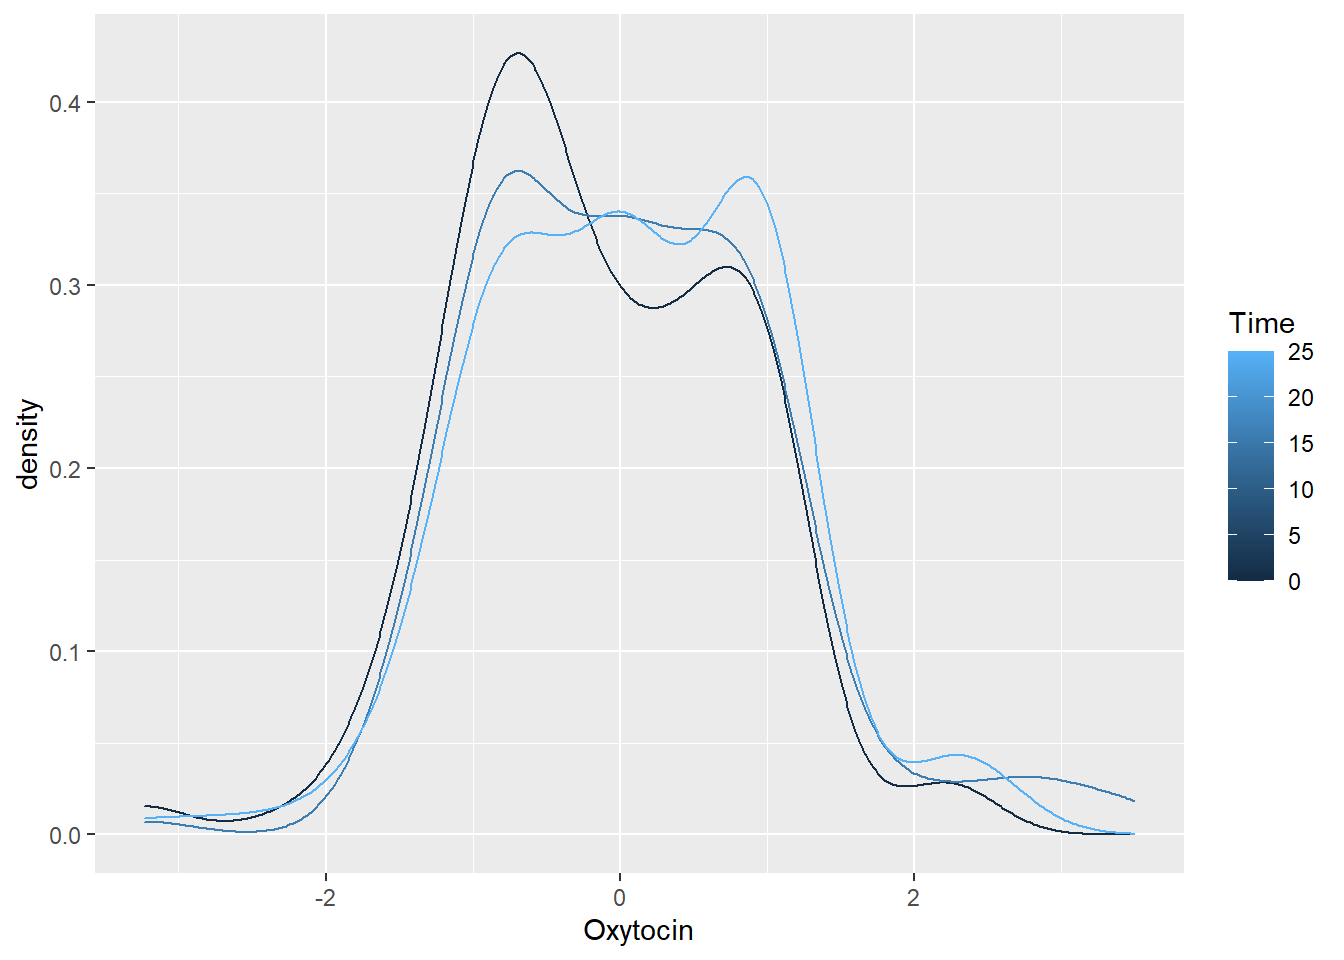
\includegraphics{01_Preprocessing_Modelling_files/figure-latex/wrap_res_OXT_2-1.pdf}

\begin{Shaded}
\begin{Highlighting}[]
\FunctionTok{ggplot}\NormalTok{(}\AttributeTok{data =}\NormalTok{ resall[[}\FunctionTok{paste0}\NormalTok{(depvar, }\StringTok{"\_longdat"}\NormalTok{)]], }
       \FunctionTok{aes}\NormalTok{(Time,DV, }\AttributeTok{col=}\NormalTok{group)) }\SpecialCharTok{+} 
  \FunctionTok{ylab}\NormalTok{(labeltag) }\SpecialCharTok{+} \FunctionTok{xlab}\NormalTok{(}\StringTok{"Time"}\NormalTok{)}\SpecialCharTok{+}
  \FunctionTok{geom\_smooth}\NormalTok{(}\AttributeTok{method =} \StringTok{\textquotesingle{}loess\textquotesingle{}}\NormalTok{) }\SpecialCharTok{+} \FunctionTok{geom\_point}\NormalTok{() }\SpecialCharTok{+}   \FunctionTok{facet\_wrap}\NormalTok{(}\SpecialCharTok{\textasciitilde{}}\NormalTok{gender)}
\end{Highlighting}
\end{Shaded}

\begin{verbatim}
## `geom_smooth()` using formula 'y ~ x'
\end{verbatim}

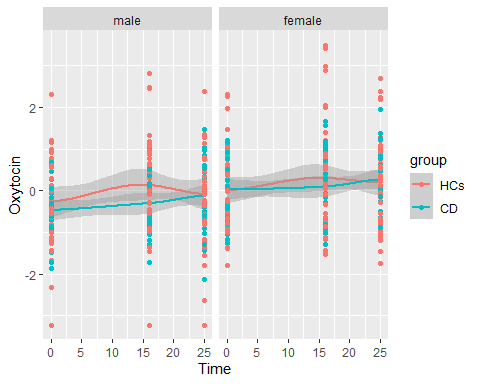
\includegraphics{01_Preprocessing_Modelling_files/figure-latex/wrap_res_OXT_2-2.pdf}

\hypertarget{sensitivity-analyses-4}{%
\paragraph{sensitivity analyses}\label{sensitivity-analyses-4}}

\begin{Shaded}
\begin{Highlighting}[]
\NormalTok{resall[[}\FunctionTok{paste0}\NormalTok{(depvar, }\StringTok{"\_coeff"}\NormalTok{)]] }\SpecialCharTok{\%\textgreater{}\%} \FunctionTok{tableplot}\NormalTok{()}
\end{Highlighting}
\end{Shaded}

\begin{table}
\centering
\begin{tabular}[t]{l|l|l|l|l}
\hline
  & Estimate & Std. Error & t value & pvalue\\
\hline
(Intercept) & -0.126 & 0.143 & -0.88 & 0.379\\
\hline
age\_meancentered & 0.0933 & 0.0781 & 1.19 & 0.232\\
\hline
explstart\_meancentered\_min & 0.0142 & 0.0933 & 0.153 & 0.879\\
\hline
BMI\_imp\_meancentered & -0.0846 & 0.0647 & -1.31 & 0.191\\
\hline
any\_med\_cceptmed & 0.0183 & 0.176 & 0.104 & 0.917\\
\hline
smoking\_yes\_nosmk & 0.185 & 0.187 & 0.987 & 0.323\\
\hline
genderfemale & 0.265 & 0.189 & 1.4 & 0.161\\
\hline
groupCD & -0.259 & 0.218 & -1.19 & 0.235\\
\hline
poly(Time, 2)1 & 2.85 & 1.47 & 1.94 & 0.0521\\
\hline
poly(Time, 2)2 & -3.96 & 1.47 & -2.7 & 0.00699\\
\hline
genderfemale:groupCD & 0.187 & 0.284 & 0.659 & 0.51\\
\hline
groupCD:poly(Time, 2)1 & 1.29 & 2.17 & 0.596 & 0.551\\
\hline
groupCD:poly(Time, 2)2 & 4.77 & 2.17 & 2.2 & 0.0277\\
\hline
genderfemale:poly(Time, 2)1 & -0.184 & 1.99 & -0.0923 & 0.926\\
\hline
genderfemale:poly(Time, 2)2 & 1.53 & 1.99 & 0.766 & 0.444\\
\hline
genderfemale:groupCD:poly(Time, 2)1 & -1.22 & 2.91 & -0.418 & 0.676\\
\hline
genderfemale:groupCD:poly(Time, 2)2 & -1.16 & 2.91 & -0.398 & 0.69\\
\hline
\end{tabular}
\end{table}

\begin{Shaded}
\begin{Highlighting}[]
\NormalTok{resall[[}\FunctionTok{paste0}\NormalTok{(depvar, }\StringTok{"\_coeff\_CDquant"}\NormalTok{)]] }\SpecialCharTok{\%\textgreater{}\%} \FunctionTok{tableplot}\NormalTok{()}
\end{Highlighting}
\end{Shaded}

\begin{table}
\centering
\begin{tabular}[t]{l|l|l|l|l}
\hline
  & Estimate & Std. Error & t value & pvalue\\
\hline
(Intercept) & -0.232 & 0.122 & -1.89 & 0.0585\\
\hline
age\_meancentered & 0.104 & 0.0773 & 1.34 & 0.18\\
\hline
explstart\_meancentered\_min & -0.000698 & 0.0923 & -0.00756 & 0.994\\
\hline
BMI\_imp\_meancentered & -0.0891 & 0.0639 & -1.39 & 0.163\\
\hline
any\_med\_cceptmed & 0.0104 & 0.177 & 0.059 & 0.953\\
\hline
smoking\_yes\_nosmk & 0.15 & 0.193 & 0.778 & 0.436\\
\hline
genderfemale & 0.351 & 0.143 & 2.45 & 0.0142\\
\hline
CDsymptomscurrent & -0.0111 & 0.109 & -0.102 & 0.919\\
\hline
poly(Time, 2)1 & 3.42 & 1.08 & 3.16 & 0.00158\\
\hline
poly(Time, 2)2 & -1.83 & 1.08 & -1.69 & 0.0911\\
\hline
genderfemale:CDsymptomscurrent & -0.0357 & 0.138 & -0.259 & 0.795\\
\hline
CDsymptomscurrent:poly(Time, 2)1 & 0.77 & 1.05 & 0.735 & 0.462\\
\hline
CDsymptomscurrent:poly(Time, 2)2 & 1.68 & 1.05 & 1.6 & 0.109\\
\hline
genderfemale:poly(Time, 2)1 & -0.713 & 1.46 & -0.49 & 0.624\\
\hline
genderfemale:poly(Time, 2)2 & 1.07 & 1.46 & 0.734 & 0.463\\
\hline
genderfemale:CDsymptomscurrent:poly(Time, 2)1 & -0.832 & 1.45 & -0.575 & 0.565\\
\hline
genderfemale:CDsymptomscurrent:poly(Time, 2)2 & 0.264 & 1.45 & 0.182 & 0.856\\
\hline
\end{tabular}
\end{table}

\begin{Shaded}
\begin{Highlighting}[]
\NormalTok{resall[[}\FunctionTok{paste0}\NormalTok{(depvar, }\StringTok{"\_coeff\_males"}\NormalTok{)]] }\SpecialCharTok{\%\textgreater{}\%} \FunctionTok{tableplot}\NormalTok{()}
\end{Highlighting}
\end{Shaded}

\begin{table}
\centering
\begin{tabular}[t]{l|l|l|l|l}
\hline
  & Estimate & Std. Error & t value & pvalue\\
\hline
(Intercept) & -0.153 & 0.153 & -0.998 & 0.318\\
\hline
age\_meancentered & -0.0353 & 0.125 & -0.282 & 0.778\\
\hline
explstart\_meancentered\_min & -0.00876 & 0.147 & -0.0594 & 0.953\\
\hline
BMI\_imp\_meancentered & 0.0166 & 0.139 & 0.12 & 0.905\\
\hline
any\_med\_cceptmed & -0.596 & 0.312 & -1.91 & 0.0559\\
\hline
smoking\_yes\_nosmk & 0.606 & 0.286 & 2.12 & 0.0343\\
\hline
groupCD & -0.309 & 0.238 & -1.3 & 0.195\\
\hline
poly(Time, 2)1 & 2.85 & 1.44 & 1.99 & 0.0471\\
\hline
poly(Time, 2)2 & -3.96 & 1.44 & -2.76 & 0.00583\\
\hline
groupCD:poly(Time, 2)1 & 1.29 & 2.12 & 0.609 & 0.543\\
\hline
groupCD:poly(Time, 2)2 & 4.77 & 2.12 & 2.25 & 0.0244\\
\hline
\end{tabular}
\end{table}

\begin{Shaded}
\begin{Highlighting}[]
\NormalTok{resall[[}\FunctionTok{paste0}\NormalTok{(depvar, }\StringTok{"\_coeff\_females"}\NormalTok{)]] }\SpecialCharTok{\%\textgreater{}\%} \FunctionTok{tableplot}\NormalTok{()}
\end{Highlighting}
\end{Shaded}

\begin{table}
\centering
\begin{tabular}[t]{l|l|l|l|l}
\hline
  & Estimate & Std. Error & t value & pvalue\\
\hline
(Intercept) & 0.0267 & 0.172 & 0.155 & 0.877\\
\hline
age\_meancentered & 0.096 & 0.105 & 0.916 & 0.359\\
\hline
explstart\_meancentered\_min & -0.0345 & 0.12 & -0.289 & 0.773\\
\hline
BMI\_imp\_meancentered & -0.137 & 0.0711 & -1.93 & 0.0539\\
\hline
any\_med\_cceptmed & 0.261 & 0.222 & 1.18 & 0.24\\
\hline
smoking\_yes\_nosmk & -0.116 & 0.256 & -0.455 & 0.649\\
\hline
groupCD & 0.00959 & 0.256 & 0.0375 & 0.97\\
\hline
poly(Time, 2)1 & 2.67 & 1.37 & 1.95 & 0.0508\\
\hline
poly(Time, 2)2 & -2.44 & 1.37 & -1.78 & 0.0745\\
\hline
groupCD:poly(Time, 2)1 & 0.0736 & 1.98 & 0.0372 & 0.97\\
\hline
groupCD:poly(Time, 2)2 & 3.61 & 1.98 & 1.83 & 0.0678\\
\hline
\end{tabular}
\end{table}

\begin{Shaded}
\begin{Highlighting}[]
\NormalTok{resall[[}\FunctionTok{paste0}\NormalTok{(depvar, }\StringTok{"\_coeff\_iq\_e\_total\_imp\_meancentered"}\NormalTok{)]] }\SpecialCharTok{\%\textgreater{}\%} \FunctionTok{tableplot}\NormalTok{()}
\end{Highlighting}
\end{Shaded}

\begin{table}
\centering
\begin{tabular}[t]{l|l|l|l|l}
\hline
  & Estimate & Std. Error & t value & pvalue\\
\hline
(Intercept) & -0.0874 & 0.148 & -0.591 & 0.554\\
\hline
iq\_e\_total\_imp\_meancentered & -0.0761 & 0.0716 & -1.06 & 0.288\\
\hline
age\_meancentered & 0.0865 & 0.0783 & 1.1 & 0.269\\
\hline
explstart\_meancentered\_min & 0.0145 & 0.0932 & 0.155 & 0.877\\
\hline
BMI\_imp\_meancentered & -0.0876 & 0.0648 & -1.35 & 0.176\\
\hline
any\_med\_cceptmed & 0.0366 & 0.177 & 0.207 & 0.836\\
\hline
smoking\_yes\_nosmk & 0.166 & 0.188 & 0.883 & 0.377\\
\hline
genderfemale & 0.219 & 0.194 & 1.13 & 0.258\\
\hline
groupCD & -0.293 & 0.22 & -1.33 & 0.184\\
\hline
poly(Time, 2)1 & 2.85 & 1.47 & 1.94 & 0.0521\\
\hline
poly(Time, 2)2 & -3.96 & 1.47 & -2.7 & 0.00699\\
\hline
genderfemale:groupCD & 0.185 & 0.284 & 0.651 & 0.515\\
\hline
groupCD:poly(Time, 2)1 & 1.29 & 2.17 & 0.596 & 0.551\\
\hline
groupCD:poly(Time, 2)2 & 4.77 & 2.17 & 2.2 & 0.0277\\
\hline
genderfemale:poly(Time, 2)1 & -0.184 & 1.99 & -0.0923 & 0.926\\
\hline
genderfemale:poly(Time, 2)2 & 1.53 & 1.99 & 0.766 & 0.444\\
\hline
genderfemale:groupCD:poly(Time, 2)1 & -1.22 & 2.91 & -0.418 & 0.676\\
\hline
genderfemale:groupCD:poly(Time, 2)2 & -1.16 & 2.91 & -0.398 & 0.69\\
\hline
\end{tabular}
\end{table}

\begin{Shaded}
\begin{Highlighting}[]
\NormalTok{resall[[}\FunctionTok{paste0}\NormalTok{(depvar, }\StringTok{"\_coeff\_EduParentsISCEDMean\_meancentered"}\NormalTok{)]] }\SpecialCharTok{\%\textgreater{}\%} \FunctionTok{tableplot}\NormalTok{()}
\end{Highlighting}
\end{Shaded}

\begin{table}
\centering
\begin{tabular}[t]{l|l|l|l|l}
\hline
  & Estimate & Std. Error & t value & pvalue\\
\hline
(Intercept) & -0.134 & 0.151 & -0.887 & 0.375\\
\hline
EduParentsISCEDMean\_meancentered & 0.0612 & 0.0795 & 0.77 & 0.442\\
\hline
age\_meancentered & 0.141 & 0.0861 & 1.63 & 0.103\\
\hline
explstart\_meancentered\_min & 0.0464 & 0.111 & 0.419 & 0.675\\
\hline
BMI\_imp\_meancentered & -0.0693 & 0.0872 & -0.795 & 0.427\\
\hline
any\_med\_cceptmed & -0.107 & 0.199 & -0.537 & 0.591\\
\hline
smoking\_yes\_nosmk & 0.205 & 0.202 & 1.01 & 0.311\\
\hline
genderfemale & 0.352 & 0.203 & 1.73 & 0.0832\\
\hline
groupCD & -0.248 & 0.233 & -1.06 & 0.287\\
\hline
poly(Time, 2)1 & 2.89 & 1.6 & 1.8 & 0.0713\\
\hline
poly(Time, 2)2 & -4.26 & 1.6 & -2.66 & 0.00788\\
\hline
genderfemale:groupCD & 0.261 & 0.315 & 0.829 & 0.407\\
\hline
groupCD:poly(Time, 2)1 & 1.16 & 2.39 & 0.488 & 0.626\\
\hline
groupCD:poly(Time, 2)2 & 5.3 & 2.39 & 2.22 & 0.0266\\
\hline
genderfemale:poly(Time, 2)1 & -0.338 & 2.24 & -0.151 & 0.88\\
\hline
genderfemale:poly(Time, 2)2 & 1.17 & 2.24 & 0.524 & 0.601\\
\hline
genderfemale:groupCD:poly(Time, 2)1 & -0.817 & 3.32 & -0.246 & 0.805\\
\hline
genderfemale:groupCD:poly(Time, 2)2 & -1.47 & 3.32 & -0.442 & 0.659\\
\hline
\end{tabular}
\end{table}

\begin{Shaded}
\begin{Highlighting}[]
\NormalTok{resall[[}\FunctionTok{paste0}\NormalTok{(depvar, }\StringTok{"\_coeff\_pubcatimp\_meancentered"}\NormalTok{)]] }\SpecialCharTok{\%\textgreater{}\%} \FunctionTok{tableplot}\NormalTok{()}
\end{Highlighting}
\end{Shaded}

\begin{table}
\centering
\begin{tabular}[t]{l|l|l|l|l}
\hline
  & Estimate & Std. Error & t value & pvalue\\
\hline
(Intercept) & -0.0588 & 0.168 & -0.35 & 0.727\\
\hline
pubcatimp\_meancentered & 0.081 & 0.106 & 0.767 & 0.443\\
\hline
age\_meancentered & 0.0482 & 0.0978 & 0.493 & 0.622\\
\hline
explstart\_meancentered\_min & 0.0251 & 0.0944 & 0.265 & 0.791\\
\hline
BMI\_imp\_meancentered & -0.0869 & 0.0649 & -1.34 & 0.181\\
\hline
any\_med\_cceptmed & 0.0034 & 0.178 & 0.0191 & 0.985\\
\hline
smoking\_yes\_nosmk & 0.161 & 0.19 & 0.852 & 0.394\\
\hline
genderfemale & 0.177 & 0.222 & 0.798 & 0.425\\
\hline
groupCD & -0.27 & 0.219 & -1.23 & 0.218\\
\hline
poly(Time, 2)1 & 2.85 & 1.47 & 1.94 & 0.0521\\
\hline
poly(Time, 2)2 & -3.96 & 1.47 & -2.7 & 0.00699\\
\hline
genderfemale:groupCD & 0.208 & 0.286 & 0.728 & 0.467\\
\hline
groupCD:poly(Time, 2)1 & 1.29 & 2.17 & 0.596 & 0.551\\
\hline
groupCD:poly(Time, 2)2 & 4.77 & 2.17 & 2.2 & 0.0277\\
\hline
genderfemale:poly(Time, 2)1 & -0.184 & 1.99 & -0.0923 & 0.926\\
\hline
genderfemale:poly(Time, 2)2 & 1.53 & 1.99 & 0.766 & 0.444\\
\hline
genderfemale:groupCD:poly(Time, 2)1 & -1.22 & 2.91 & -0.418 & 0.676\\
\hline
genderfemale:groupCD:poly(Time, 2)2 & -1.16 & 2.91 & -0.398 & 0.69\\
\hline
\end{tabular}
\end{table}

\begin{Shaded}
\begin{Highlighting}[]
\NormalTok{resall[[}\FunctionTok{paste0}\NormalTok{(depvar, }\StringTok{"\_coeff\_ADHD\_life"}\NormalTok{)]] }\SpecialCharTok{\%\textgreater{}\%} \FunctionTok{tableplot}\NormalTok{()}
\end{Highlighting}
\end{Shaded}

\begin{table}
\centering
\begin{tabular}[t]{l|l|l|l|l}
\hline
  & Estimate & Std. Error & t value & pvalue\\
\hline
(Intercept) & -0.135 & 0.143 & -0.943 & 0.346\\
\hline
ADHD\_lifeADHD & 0.258 & 0.208 & 1.24 & 0.216\\
\hline
age\_meancentered & 0.0941 & 0.0779 & 1.21 & 0.227\\
\hline
explstart\_meancentered\_min & 0.0155 & 0.0931 & 0.166 & 0.868\\
\hline
BMI\_imp\_meancentered & -0.0914 & 0.0649 & -1.41 & 0.159\\
\hline
any\_med\_cceptmed & 0.0311 & 0.176 & 0.176 & 0.86\\
\hline
smoking\_yes\_nosmk & 0.224 & 0.189 & 1.18 & 0.236\\
\hline
genderfemale & 0.27 & 0.189 & 1.43 & 0.153\\
\hline
groupCD & -0.436 & 0.261 & -1.67 & 0.0941\\
\hline
poly(Time, 2)1 & 2.85 & 1.47 & 1.94 & 0.0521\\
\hline
poly(Time, 2)2 & -3.96 & 1.47 & -2.7 & 0.00699\\
\hline
genderfemale:groupCD & 0.251 & 0.289 & 0.87 & 0.384\\
\hline
groupCD:poly(Time, 2)1 & 1.29 & 2.17 & 0.596 & 0.551\\
\hline
groupCD:poly(Time, 2)2 & 4.77 & 2.17 & 2.2 & 0.0277\\
\hline
genderfemale:poly(Time, 2)1 & -0.184 & 1.99 & -0.0923 & 0.926\\
\hline
genderfemale:poly(Time, 2)2 & 1.53 & 1.99 & 0.766 & 0.444\\
\hline
genderfemale:groupCD:poly(Time, 2)1 & -1.22 & 2.91 & -0.418 & 0.676\\
\hline
genderfemale:groupCD:poly(Time, 2)2 & -1.16 & 2.91 & -0.398 & 0.69\\
\hline
\end{tabular}
\end{table}

\begin{Shaded}
\begin{Highlighting}[]
\NormalTok{resall[[}\FunctionTok{paste0}\NormalTok{(depvar, }\StringTok{"\_coeff\_Depression\_lifetime"}\NormalTok{)]] }\SpecialCharTok{\%\textgreater{}\%} \FunctionTok{tableplot}\NormalTok{()}
\end{Highlighting}
\end{Shaded}

\begin{table}
\centering
\begin{tabular}[t]{l|l|l|l|l}
\hline
  & Estimate & Std. Error & t value & pvalue\\
\hline
(Intercept) & -0.131 & 0.144 & -0.909 & 0.363\\
\hline
Depression\_lifetimeDepression & -0.114 & 0.211 & -0.54 & 0.589\\
\hline
age\_meancentered & 0.0917 & 0.0783 & 1.17 & 0.241\\
\hline
explstart\_meancentered\_min & 0.016 & 0.0935 & 0.172 & 0.864\\
\hline
BMI\_imp\_meancentered & -0.0898 & 0.0656 & -1.37 & 0.171\\
\hline
any\_med\_cceptmed & 0.0423 & 0.182 & 0.232 & 0.817\\
\hline
smoking\_yes\_nosmk & 0.198 & 0.189 & 1.05 & 0.294\\
\hline
genderfemale & 0.269 & 0.19 & 1.42 & 0.156\\
\hline
groupCD & -0.243 & 0.221 & -1.1 & 0.272\\
\hline
poly(Time, 2)1 & 2.85 & 1.47 & 1.94 & 0.0521\\
\hline
poly(Time, 2)2 & -3.96 & 1.47 & -2.7 & 0.00699\\
\hline
genderfemale:groupCD & 0.205 & 0.287 & 0.714 & 0.475\\
\hline
groupCD:poly(Time, 2)1 & 1.29 & 2.17 & 0.596 & 0.551\\
\hline
groupCD:poly(Time, 2)2 & 4.77 & 2.17 & 2.2 & 0.0277\\
\hline
genderfemale:poly(Time, 2)1 & -0.184 & 1.99 & -0.0923 & 0.926\\
\hline
genderfemale:poly(Time, 2)2 & 1.53 & 1.99 & 0.766 & 0.444\\
\hline
genderfemale:groupCD:poly(Time, 2)1 & -1.22 & 2.91 & -0.418 & 0.676\\
\hline
genderfemale:groupCD:poly(Time, 2)2 & -1.16 & 2.91 & -0.398 & 0.69\\
\hline
\end{tabular}
\end{table}

\begin{Shaded}
\begin{Highlighting}[]
\NormalTok{resall[[}\FunctionTok{paste0}\NormalTok{(depvar, }\StringTok{"\_coeff\_PTSD\_lifetime"}\NormalTok{)]] }\SpecialCharTok{\%\textgreater{}\%} \FunctionTok{tableplot}\NormalTok{()}
\end{Highlighting}
\end{Shaded}

\begin{table}
\centering
\begin{tabular}[t]{l|l|l|l|l}
\hline
  & Estimate & Std. Error & t value & pvalue\\
\hline
(Intercept) & -0.12 & 0.142 & -0.847 & 0.397\\
\hline
PTSD\_lifetimePTSD & -0.544 & 0.255 & -2.14 & 0.0327\\
\hline
age\_meancentered & 0.0972 & 0.0772 & 1.26 & 0.208\\
\hline
explstart\_meancentered\_min & 0.00776 & 0.0923 & 0.0841 & 0.933\\
\hline
BMI\_imp\_meancentered & -0.0825 & 0.064 & -1.29 & 0.197\\
\hline
any\_med\_cceptmed & 0.0531 & 0.175 & 0.303 & 0.762\\
\hline
smoking\_yes\_nosmk & 0.215 & 0.185 & 1.16 & 0.246\\
\hline
genderfemale & 0.255 & 0.187 & 1.36 & 0.174\\
\hline
groupCD & -0.21 & 0.217 & -0.967 & 0.334\\
\hline
poly(Time, 2)1 & 2.85 & 1.47 & 1.94 & 0.0521\\
\hline
poly(Time, 2)2 & -3.96 & 1.47 & -2.7 & 0.00699\\
\hline
genderfemale:groupCD & 0.199 & 0.281 & 0.709 & 0.479\\
\hline
groupCD:poly(Time, 2)1 & 1.29 & 2.17 & 0.596 & 0.551\\
\hline
groupCD:poly(Time, 2)2 & 4.77 & 2.17 & 2.2 & 0.0277\\
\hline
genderfemale:poly(Time, 2)1 & -0.184 & 1.99 & -0.0923 & 0.926\\
\hline
genderfemale:poly(Time, 2)2 & 1.53 & 1.99 & 0.766 & 0.444\\
\hline
genderfemale:groupCD:poly(Time, 2)1 & -1.22 & 2.91 & -0.418 & 0.676\\
\hline
genderfemale:groupCD:poly(Time, 2)2 & -1.16 & 2.91 & -0.398 & 0.69\\
\hline
\end{tabular}
\end{table}

\begin{Shaded}
\begin{Highlighting}[]
\NormalTok{resall[[}\FunctionTok{paste0}\NormalTok{(depvar, }\StringTok{"\_coeff\_SUD\_life"}\NormalTok{)]] }\SpecialCharTok{\%\textgreater{}\%} \FunctionTok{tableplot}\NormalTok{()}
\end{Highlighting}
\end{Shaded}

\begin{table}
\centering
\begin{tabular}[t]{l|l|l|l|l}
\hline
  & Estimate & Std. Error & t value & pvalue\\
\hline
(Intercept) & -0.119 & 0.144 & -0.832 & 0.406\\
\hline
SUD\_lifeSUD & 0.217 & 0.25 & 0.866 & 0.387\\
\hline
age\_meancentered & 0.0841 & 0.0788 & 1.07 & 0.286\\
\hline
explstart\_meancentered\_min & 0.00634 & 0.0938 & 0.0676 & 0.946\\
\hline
BMI\_imp\_meancentered & -0.079 & 0.0651 & -1.21 & 0.225\\
\hline
any\_med\_cceptmed & 0.0014 & 0.178 & 0.00786 & 0.994\\
\hline
smoking\_yes\_nosmk & 0.117 & 0.203 & 0.576 & 0.564\\
\hline
genderfemale & 0.263 & 0.189 & 1.39 & 0.164\\
\hline
groupCD & -0.295 & 0.222 & -1.33 & 0.185\\
\hline
poly(Time, 2)1 & 2.85 & 1.47 & 1.94 & 0.0521\\
\hline
poly(Time, 2)2 & -3.96 & 1.47 & -2.7 & 0.00699\\
\hline
genderfemale:groupCD & 0.213 & 0.286 & 0.746 & 0.456\\
\hline
groupCD:poly(Time, 2)1 & 1.29 & 2.17 & 0.596 & 0.551\\
\hline
groupCD:poly(Time, 2)2 & 4.77 & 2.17 & 2.2 & 0.0277\\
\hline
genderfemale:poly(Time, 2)1 & -0.184 & 1.99 & -0.0923 & 0.926\\
\hline
genderfemale:poly(Time, 2)2 & 1.53 & 1.99 & 0.766 & 0.444\\
\hline
genderfemale:groupCD:poly(Time, 2)1 & -1.22 & 2.91 & -0.418 & 0.676\\
\hline
genderfemale:groupCD:poly(Time, 2)2 & -1.16 & 2.91 & -0.398 & 0.69\\
\hline
\end{tabular}
\end{table}

\begin{Shaded}
\begin{Highlighting}[]
\NormalTok{resall[[}\FunctionTok{paste0}\NormalTok{(depvar, }\StringTok{"\_coeff\_Anxiety\_lifetime"}\NormalTok{)]] }\SpecialCharTok{\%\textgreater{}\%} \FunctionTok{tableplot}\NormalTok{()}
\end{Highlighting}
\end{Shaded}

\begin{table}
\centering
\begin{tabular}[t]{l|l|l|l|l}
\hline
  & Estimate & Std. Error & t value & pvalue\\
\hline
(Intercept) & -0.123 & 0.144 & -0.852 & 0.394\\
\hline
Anxiety\_lifetimeAnxiety & -0.0925 & 0.201 & -0.46 & 0.646\\
\hline
age\_meancentered & 0.0916 & 0.0784 & 1.17 & 0.243\\
\hline
explstart\_meancentered\_min & 0.014 & 0.0935 & 0.149 & 0.881\\
\hline
BMI\_imp\_meancentered & -0.0863 & 0.065 & -1.33 & 0.184\\
\hline
any\_med\_cceptmed & 0.0406 & 0.183 & 0.222 & 0.825\\
\hline
smoking\_yes\_nosmk & 0.18 & 0.188 & 0.962 & 0.336\\
\hline
genderfemale & 0.262 & 0.19 & 1.38 & 0.168\\
\hline
groupCD & -0.227 & 0.23 & -0.989 & 0.323\\
\hline
poly(Time, 2)1 & 2.85 & 1.47 & 1.94 & 0.0521\\
\hline
poly(Time, 2)2 & -3.96 & 1.47 & -2.7 & 0.00699\\
\hline
genderfemale:groupCD & 0.167 & 0.289 & 0.578 & 0.563\\
\hline
groupCD:poly(Time, 2)1 & 1.29 & 2.17 & 0.596 & 0.551\\
\hline
groupCD:poly(Time, 2)2 & 4.77 & 2.17 & 2.2 & 0.0277\\
\hline
genderfemale:poly(Time, 2)1 & -0.184 & 1.99 & -0.0923 & 0.926\\
\hline
genderfemale:poly(Time, 2)2 & 1.53 & 1.99 & 0.766 & 0.444\\
\hline
genderfemale:groupCD:poly(Time, 2)1 & -1.22 & 2.91 & -0.418 & 0.676\\
\hline
genderfemale:groupCD:poly(Time, 2)2 & -1.16 & 2.91 & -0.398 & 0.69\\
\hline
\end{tabular}
\end{table}

\begin{Shaded}
\begin{Highlighting}[]
\NormalTok{restabnames }\OtherTok{=} \FunctionTok{grep}\NormalTok{(}\StringTok{"coeff$"}\NormalTok{,}\FunctionTok{names}\NormalTok{(resall), }\AttributeTok{value=}\NormalTok{T)}
\NormalTok{resall\_mod}\OtherTok{=}\FunctionTok{lapply}\NormalTok{(resall[restabnames], tibble}\SpecialCharTok{::}\NormalTok{rownames\_to\_column)}
\NormalTok{fullres}\OtherTok{=}\NormalTok{resall\_mod }\SpecialCharTok{\%\textgreater{}\%} \FunctionTok{reduce}\NormalTok{(full\_join, }\AttributeTok{by=}\StringTok{"rowname"}\NormalTok{)}
\NormalTok{fullres }\OtherTok{=}\NormalTok{ fullres }\SpecialCharTok{\%\textgreater{}\%} \FunctionTok{select}\NormalTok{ (.,}\SpecialCharTok{{-}} \FunctionTok{grep}\NormalTok{(}\StringTok{"t value"}\NormalTok{, }\FunctionTok{colnames}\NormalTok{(fullres), }\AttributeTok{value =}\NormalTok{ T))}
\NormalTok{newnames }\OtherTok{=} \FunctionTok{c}\NormalTok{(}\StringTok{"{-}"}\NormalTok{, }\FunctionTok{rep}\NormalTok{(}\FunctionTok{c}\NormalTok{(}\StringTok{"beta"}\NormalTok{, }\StringTok{"se"}\NormalTok{, }\StringTok{"P"}\NormalTok{), }\FunctionTok{length}\NormalTok{(}\FunctionTok{names}\NormalTok{(AV))))}

\NormalTok{tableplot\_2}\OtherTok{=} \ControlFlowTok{function}\NormalTok{ (x)\{}
\NormalTok{    x }\SpecialCharTok{\%\textgreater{}\%}\NormalTok{ dplyr}\SpecialCharTok{::}\FunctionTok{mutate\_if}\NormalTok{(is.numeric, }\ControlFlowTok{function}\NormalTok{(x)\{}\FunctionTok{as.character}\NormalTok{(}\FunctionTok{signif}\NormalTok{(x, }\DecValTok{3}\NormalTok{))\}) }\SpecialCharTok{\%\textgreater{}\%} 
    \FunctionTok{kbl}\NormalTok{(.,}\AttributeTok{col.names =}\NormalTok{ newnames) }\SpecialCharTok{\%\textgreater{}\%} 
    \FunctionTok{add\_header\_above}\NormalTok{(}\FunctionTok{c}\NormalTok{(}\StringTok{"indep. variable"} \OtherTok{=} \DecValTok{1}\NormalTok{, }
                       \StringTok{"Psych. stress"}\OtherTok{=}\DecValTok{3}\NormalTok{, }
                       \StringTok{"Testosterone"}\OtherTok{=}\DecValTok{3}\NormalTok{, }
                       \StringTok{"Cortisol"}\OtherTok{=}\DecValTok{3}\NormalTok{, }
                       \StringTok{"Test/Cort ratio"}\OtherTok{=}\DecValTok{3}\NormalTok{,}
                       \StringTok{"Oxytocin"}\OtherTok{=}\DecValTok{3}\NormalTok{)) }\SpecialCharTok{\%\textgreater{}\%} \FunctionTok{kable\_classic}\NormalTok{()}
\NormalTok{\}}


\NormalTok{tableplot\_3}\OtherTok{=} \ControlFlowTok{function}\NormalTok{ (x)\{}
\NormalTok{    x }\SpecialCharTok{\%\textgreater{}\%}\NormalTok{ dplyr}\SpecialCharTok{::}\FunctionTok{mutate\_if}\NormalTok{(is.numeric, }
                           \ControlFlowTok{function}\NormalTok{(x)\{}\FunctionTok{as.character}\NormalTok{(}\FunctionTok{round}\NormalTok{(x, }\DecValTok{3}\NormalTok{))\}) }\SpecialCharTok{\%\textgreater{}\%}
    \FunctionTok{mutate\_all}\NormalTok{(}\SpecialCharTok{\textasciitilde{}}\FunctionTok{replace}\NormalTok{(., .}\SpecialCharTok{==}\StringTok{"0"}\NormalTok{, }\StringTok{"\textless{}0.001"}\NormalTok{)) }\SpecialCharTok{\%\textgreater{}\%}
    \FunctionTok{kbl}\NormalTok{(.,}\AttributeTok{col.names =}\NormalTok{ newnames) }\SpecialCharTok{\%\textgreater{}\%} 
    \FunctionTok{add\_header\_above}\NormalTok{(}\FunctionTok{c}\NormalTok{(}\StringTok{"indep. variable"} \OtherTok{=} \DecValTok{1}\NormalTok{, }
                       \StringTok{"Psych. stress"}\OtherTok{=}\DecValTok{3}\NormalTok{, }
                       \StringTok{"Testosterone"}\OtherTok{=}\DecValTok{3}\NormalTok{, }
                       \StringTok{"Cortisol"}\OtherTok{=}\DecValTok{3}\NormalTok{, }
                       \StringTok{"Test/Cort ratio"}\OtherTok{=}\DecValTok{3}\NormalTok{,}
                       \StringTok{"Oxytocin"}\OtherTok{=}\DecValTok{3}\NormalTok{)) }\SpecialCharTok{\%\textgreater{}\%} \FunctionTok{kable\_classic}\NormalTok{()}
\NormalTok{\}}
\end{Highlighting}
\end{Shaded}

\hypertarget{summary-table-main-models}{%
\subsection{summary table main models}\label{summary-table-main-models}}

\hypertarget{all-effects}{%
\subsubsection{all effects}\label{all-effects}}

\begin{Shaded}
\begin{Highlighting}[]
\CommentTok{\#fullres \%\textgreater{}\% tableplot\_2() }
\NormalTok{fullres }\SpecialCharTok{\%\textgreater{}\%} \FunctionTok{tableplot\_3}\NormalTok{() }
\end{Highlighting}
\end{Shaded}

\begin{table}
\centering
\begin{tabular}[t]{l|l|l|l|l|l|l|l|l|l|l|l|l|l|l|l}
\hline
\multicolumn{1}{c|}{indep. variable} & \multicolumn{3}{c|}{Psych. stress} & \multicolumn{3}{c|}{Testosterone} & \multicolumn{3}{c|}{Cortisol} & \multicolumn{3}{c|}{Test/Cort ratio} & \multicolumn{3}{c}{Oxytocin} \\
\cline{1-1} \cline{2-4} \cline{5-7} \cline{8-10} \cline{11-13} \cline{14-16}
- & beta & se & P & beta & se & P & beta & se & P & beta & se & P & beta & se & P\\
\hline
(Intercept) & -0.177 & 0.085 & 0.037 & 0.24 & 0.112 & 0.032 & 0.513 & 0.156 & 0.001 & -0.062 & 0.114 & 0.584 & -0.126 & 0.143 & 0.379\\
\hline
age\_meancentered & 0.039 & 0.037 & 0.301 & 0.239 & 0.051 & <0.001 & 0.238 & 0.055 & <0.001 & -0.185 & 0.052 & <0.001 & 0.093 & 0.078 & 0.232\\
\hline
genderfemale & 0.117 & 0.105 & 0.265 & -0.07 & 0.129 & 0.585 & -0.647 & 0.136 & <0.001 & 0.023 & 0.128 & 0.857 & 0.265 & 0.189 & 0.161\\
\hline
groupCD & 0.21 & 0.125 & 0.091 & -0.415 & 0.16 & 0.009 & -0.015 & 0.166 & 0.929 & 0.339 & 0.159 & 0.033 & -0.259 & 0.218 & 0.235\\
\hline
poly(Time, 2)1 & -13.46 & 1.705 & <0.001 & 0.045 & 1.233 & 0.971 & 2.177 & 0.736 & 0.003 & 0.415 & 1.676 & 0.804 & 2.854 & 1.469 & 0.052\\
\hline
poly(Time, 2)2 & 2.705 & 1.705 & 0.113 & -7.782 & 1.233 & <0.001 & -1.825 & 0.736 & 0.013 & 5.855 & 1.666 & <0.001 & -3.963 & 1.469 & 0.007\\
\hline
genderfemale:groupCD & 0.026 & 0.156 & 0.869 & 0.052 & 0.194 & 0.791 & -0.066 & 0.203 & 0.746 & -0.154 & 0.193 & 0.425 & 0.187 & 0.284 & 0.51\\
\hline
groupCD:poly(Time, 2)1 & 2.652 & 2.509 & 0.291 & -4.254 & 1.816 & 0.019 & -2.243 & 1.083 & 0.038 & 3.114 & 2.49 & 0.211 & 1.29 & 2.165 & 0.551\\
\hline
groupCD:poly(Time, 2)2 & 0.063 & 2.509 & 0.98 & 7.254 & 1.816 & <0.001 & 0.671 & 1.083 & 0.536 & -5.432 & 2.453 & 0.027 & 4.766 & 2.165 & 0.028\\
\hline
genderfemale:poly(Time, 2)1 & -2.719 & 2.114 & 0.198 & 0.948 & 1.53 & 0.536 & -1.923 & 0.913 & 0.035 & -1.519 & 2.095 & 0.468 & -0.184 & 1.991 & 0.926\\
\hline
genderfemale:poly(Time, 2)2 & 1.706 & 2.114 & 0.42 & -6.305 & 1.53 & <0.001 & -3.224 & 0.913 & <0.001 & 6.091 & 2.075 & 0.003 & 1.525 & 1.991 & 0.444\\
\hline
genderfemale:groupCD:poly(Time, 2)1 & -2.102 & 3.138 & 0.503 & 0.241 & 2.27 & 0.915 & 2.068 & 1.354 & 0.127 & 1.044 & 3.127 & 0.739 & -1.216 & 2.909 & 0.676\\
\hline
genderfemale:groupCD:poly(Time, 2)2 & -1.281 & 3.138 & 0.683 & 5.302 & 2.27 & 0.02 & 3.963 & 1.354 & 0.003 & -4.498 & 3.088 & 0.145 & -1.158 & 2.909 & 0.69\\
\hline
explstart\_meancentered\_min & NA & NA & NA & -0.177 & 0.046 & <0.001 & -0.18 & 0.048 & <0.001 & 0.16 & 0.046 & 0.001 & 0.014 & 0.093 & 0.879\\
\hline
BMI\_imp\_meancentered & NA & NA & NA & 0.049 & 0.047 & 0.301 & 0.17 & 0.049 & 0.001 & -0.029 & 0.047 & 0.54 & -0.085 & 0.065 & 0.191\\
\hline
any\_med\_cceptmed & NA & NA & NA & -0.021 & 0.122 & 0.863 & -0.207 & 0.128 & 0.105 & -0.07 & 0.122 & 0.569 & 0.018 & 0.176 & 0.917\\
\hline
smoking\_yes\_nosmk & NA & NA & NA & -0.106 & 0.125 & 0.397 & 0.162 & 0.132 & 0.219 & 0.094 & 0.125 & 0.453 & 0.185 & 0.187 & 0.323\\
\hline
\end{tabular}
\end{table}

\hypertarget{effects-of-interest}{%
\subsubsection{effects of interest}\label{effects-of-interest}}

\begin{Shaded}
\begin{Highlighting}[]
\NormalTok{index }\OtherTok{=} \FunctionTok{complete.cases}\NormalTok{(fullres) }\SpecialCharTok{\&} \SpecialCharTok{!}\NormalTok{fullres}\SpecialCharTok{$}\NormalTok{rowname }\SpecialCharTok{\%in\%} \FunctionTok{c}\NormalTok{(}\StringTok{"(Intercept)"}\NormalTok{,}\StringTok{"age\_meancentered"}\NormalTok{)}

\CommentTok{\#fullres[index,1:16] \%\textgreater{}\% as.tibble() \%\textgreater{}\% tableplot\_2()}
\NormalTok{fullres[index,}\DecValTok{1}\SpecialCharTok{:}\DecValTok{16}\NormalTok{] }\SpecialCharTok{\%\textgreater{}\%} \FunctionTok{as.tibble}\NormalTok{() }\SpecialCharTok{\%\textgreater{}\%} \FunctionTok{tableplot\_3}\NormalTok{()}
\end{Highlighting}
\end{Shaded}

\begin{table}
\centering
\begin{tabular}[t]{l|l|l|l|l|l|l|l|l|l|l|l|l|l|l|l}
\hline
\multicolumn{1}{c|}{indep. variable} & \multicolumn{3}{c|}{Psych. stress} & \multicolumn{3}{c|}{Testosterone} & \multicolumn{3}{c|}{Cortisol} & \multicolumn{3}{c|}{Test/Cort ratio} & \multicolumn{3}{c}{Oxytocin} \\
\cline{1-1} \cline{2-4} \cline{5-7} \cline{8-10} \cline{11-13} \cline{14-16}
- & beta & se & P & beta & se & P & beta & se & P & beta & se & P & beta & se & P\\
\hline
genderfemale & 0.117 & 0.105 & 0.265 & -0.07 & 0.129 & 0.585 & -0.647 & 0.136 & <0.001 & 0.023 & 0.128 & 0.857 & 0.265 & 0.189 & 0.161\\
\hline
groupCD & 0.21 & 0.125 & 0.091 & -0.415 & 0.16 & 0.009 & -0.015 & 0.166 & 0.929 & 0.339 & 0.159 & 0.033 & -0.259 & 0.218 & 0.235\\
\hline
poly(Time, 2)1 & -13.46 & 1.705 & <0.001 & 0.045 & 1.233 & 0.971 & 2.177 & 0.736 & 0.003 & 0.415 & 1.676 & 0.804 & 2.854 & 1.469 & 0.052\\
\hline
poly(Time, 2)2 & 2.705 & 1.705 & 0.113 & -7.782 & 1.233 & <0.001 & -1.825 & 0.736 & 0.013 & 5.855 & 1.666 & <0.001 & -3.963 & 1.469 & 0.007\\
\hline
genderfemale:groupCD & 0.026 & 0.156 & 0.869 & 0.052 & 0.194 & 0.791 & -0.066 & 0.203 & 0.746 & -0.154 & 0.193 & 0.425 & 0.187 & 0.284 & 0.51\\
\hline
groupCD:poly(Time, 2)1 & 2.652 & 2.509 & 0.291 & -4.254 & 1.816 & 0.019 & -2.243 & 1.083 & 0.038 & 3.114 & 2.49 & 0.211 & 1.29 & 2.165 & 0.551\\
\hline
groupCD:poly(Time, 2)2 & 0.063 & 2.509 & 0.98 & 7.254 & 1.816 & <0.001 & 0.671 & 1.083 & 0.536 & -5.432 & 2.453 & 0.027 & 4.766 & 2.165 & 0.028\\
\hline
genderfemale:poly(Time, 2)1 & -2.719 & 2.114 & 0.198 & 0.948 & 1.53 & 0.536 & -1.923 & 0.913 & 0.035 & -1.519 & 2.095 & 0.468 & -0.184 & 1.991 & 0.926\\
\hline
genderfemale:poly(Time, 2)2 & 1.706 & 2.114 & 0.42 & -6.305 & 1.53 & <0.001 & -3.224 & 0.913 & <0.001 & 6.091 & 2.075 & 0.003 & 1.525 & 1.991 & 0.444\\
\hline
genderfemale:groupCD:poly(Time, 2)1 & -2.102 & 3.138 & 0.503 & 0.241 & 2.27 & 0.915 & 2.068 & 1.354 & 0.127 & 1.044 & 3.127 & 0.739 & -1.216 & 2.909 & 0.676\\
\hline
genderfemale:groupCD:poly(Time, 2)2 & -1.281 & 3.138 & 0.683 & 5.302 & 2.27 & 0.02 & 3.963 & 1.354 & 0.003 & -4.498 & 3.088 & 0.145 & -1.158 & 2.909 & 0.69\\
\hline
\end{tabular}
\end{table}

\end{document}
